\documentclass[letter]{report}
\usepackage{graphicx}
\usepackage{amssymb}
\usepackage{hyperref}
\usepackage{listings}
\usepackage{color}

\usepackage{epstopdf}
\usepackage{geometry}
\usepackage{anysize}

%\input{config.tex}

\pagestyle{empty}
\setcounter{secnumdepth}{3}

\title{ {\LARGE\bf
        MESQUITE \\ Mesh Quality Improvement Toolkit \\ \vspace{.5cm} User's Guide\\
}}

\author{Patrick Knupp \\
The Sandia National Laboratories \\
Albuquerque NM USA \\
 \\
Lori Freitag-Diachin \\
Livermore National Laboratory \\
Livermore CA USA \\
%  \\
%Thomas Leurent \\
%Argonne National Laboratory \\
%Argonne, IL 60490 USA \\
  \\
Boyd Tidwell \\
Elemental Technologies Inc. \\
American Fork, UT USA}

\date{Last Updated: 17 May, 2013}

\begin{document}

\lstset{language=C++}

% Define a special delimiters \< and \> such that any source
% code in a listing that is between such delimiters will be
% epmhasized.  These delimiters are then used to emphasize
% differences between versions of source code.
\lstset{moredelim=[is][\color{blue}]{\\<}{\\>}}

\maketitle

\tableofcontents

%\listoffigures

%\listoftables

% Introduction to Mesquite
\chapter{Introduction to Mesquite} \label{sec:intro}

\section{Overview of Mesh Quality}

\hskip 0.25in {\it Mesh quality} refers to geometric properties of a mesh such as 
local volume, smoothness, shape, and orientation that, if not properly 
controlled, 
can adversely affect solution accuracy or computational efficiency of numerical simulations. In this section we give an overview of the role of mesh quality 
in the context of computer simulations of physical phenomena. \newline

Simulation of many phenomena in the physical world involves computing 
numerical 
solutions to partial differential equations (PDE's). Commonly used approaches 
to computing  numerical solutions such as finite volume and finite 
element methods require the use of approximations to the continuum operators 
in the PDE and a mesh or grid to subdivide the physical domain into small 
subregions. Together, the approximations and the mesh define a discretization. 
The difference between the exact solution to the PDE and the numerical solution is known as the discretization error. A {\it convergent} 
discretization means that the discretization error will asymptotically 
approach zero as the characteristic mesh size ``h'' 
approaches zero. Decreasing mesh size to reduce discretization error to 
nearly zero is often impractical in realistic simulations due to limited 
computing resources. One way to increase the accuracy of simulations with the 
same computer resources is to {\it adapt} the mesh to the domain and to the 
numerical solution. In adaptive refinement, the local mesh volume (or size) 
is made smaller in locations where the local discretization error is large and 
is made larger in locations where the error is small. In local h-refinement, 
mesh volume is made smaller by locally subdividing the mesh. In 
r-refinement, mesh volume is made smaller by moving mesh nodes closer together.
Geometric adaptation can also be important in improving simulation accuracy. In regions of high domain curvature one adapts the mesh to the domain geometry by creating locally smaller mesh sizes. We see, then, that local mesh size (or volume) is a critical parameter in determining the accuracy of a simulation. \newline

Aside from local mesh size, several other geometric mesh properties can affect 
solution accuracy. These include mesh smoothness, local mesh angles, aspect 
ratio, and orientation. For example, in some discretization methods there will be a 
loss of accuracy if the mesh is not smooth.  In other cases, aspect ratios and 
orientation must be carefully adapted to the solution in order to maintain a 
certain level of accuracy. Simulations using meshes or domains that evolve 
in time (such as in ALE simulations) usually require that initially good 
geometric mesh properties be retained throughout the simulation time period. 
It is thus often important to control other geometric mesh properties in addition to local mesh size within an adaptive simulation. \newline

In addition to solution accuracy, geometric mesh properties can also affect the amount of computer time required to obtain the numerical solution. Simulation codes usually employ iterative solvers to solve systems of equations and thus obtain numerical solutions to PDE's. The rate at which these solvers converge is determined by the spectral radius of a certain matrix. The spectral radius of the matrix is affected by, among other things, geometric properties of the mesh. Poor mesh quality can thus adversely impact solution efficiency. \newline

Adaptive meshing techniques require an initial mesh to begin the adaptation procedure. Poor quality of the initial mesh (relative to the adapted mesh) can be difficult to overcome or, at least, reduce the efficiency of 
the adaptive procedure. For example, if the initial mesh contains locally inverted elements, these can often be fixed before the adaptive procedure begins. As another example, if it is known \`{a} priori that small angles will be needed on the boundary of the domain to obtain reasonable simulation accuracy, one should try to first create the small angles in the initial mesh to improve the efficiency of the subsequent adaptive meshing procedure. \newline


Many simulations, particularly those in industry, are performed in a 
non-adaptive setting. That is to say, an initial mesh is generated and
used throughout the calculation. The mesh is not changed as the solution
is computed. Mesh quality remains important for such calculations. First, 
for complicated geometric domains it is often difficult to obtain good 
initial mesh quality. This is particularly true for non-simplicial meshes 
but can be true for simplicial meshes as well. A common requirement is that the mesh be smooth. Many simulation codes will not run to completion if the initial mesh contains a local volume which is negative. These must be eliminated before a simulation can begin. Analysts performing 
non-adaptive calculations often have considerable experience in using a variety
of meshes on their problem and have a good \`{a} priori idea of what constitutes
good mesh quality for a given problem. They thus desire to control the usual
geometric mesh properties of the non-adapted mesh carefully. 



\section{How Mesh Quality Is Improved}
Mesh quality can and should be considered during many stages of 
the mesh generation process from de-featuring CAD models to  
creation and adaptation of the mesh. Thus, for example, certain
non-essential features of a CAD model, if eliminated, would go a 
long way to improving the quality of the mesh, depending upon
the meshing scheme. Other critical meshing parameters which can 
affect mesh quality include geometric domain partitions, interval size
and count, interaction of meshes within large assemblies of parts, 
biasing requirements, corner picking, etc. Choices made during the 
mesh generation phase of an analysis may have a large impact on 
initial mesh quality.  Mesh quality can thus be improved by changing the 
way in which the domain is meshed. \newline

Once the meshing stage is completed, one can improve mesh quality
by techniques such as vertex movement and local topology modification.
In vertex movement schemes, one seeks to reposition existing mesh vertices to 
achieve better quality. If vertex movement is undertaken within an adaptive 
setting, it is commonly referred to as r-refinement. 
Classic examples of vertex movement methods 
include Laplace smoothing \cite{F88} and Winslow smoothing \cite{Winslow}. 
It is helpful, in vertex movement schemes, to first be 
able to measure mesh quality so that one can explain in what sense one 
has improved it. Given a {\it metric} to measure mesh quality, 
one can formulate a numerical 
optimization problem which guides vertex movement to find the optimal 
mesh and thus improve its quality.  Numerical 
optimization methods recently
developed for unstructured meshes include \cite{Opt-MS,Kn00,FrKn01,
FeasNewt,bjoe:swap,bjoe:chain-swap,es92}. We refer the reader to ref xxx
which is a survey of mesh quality improvement methods which have appeared 
in the literature. \newline

A large number of mesh quality metrics have been devised to measure 
mesh quality. Many of these metrics are independent of any solution 
properties and are thus not useful in adaptive meshing. However, there
are a number of weighted quality metrics which can be tied to the 
numerical solution via error indicators or other information for adaptive 
meshing. Examples of weighted metrics which have or could be used in 
adaptive calculations include those of Brackbill (ref), Knupp (ref), etc. \newline

Another way to improve mesh quality is to use local topological modification methods in which mesh vertices or elements are locally created and/or destroyed. These methods are very successful when applied to simplicial meshes, often within an adaptive context.  Local topology modification is less effective on non-simplicial meshes. \newline

Mesh quality improvement remains an important on-going research area. 
There remain, for example, open questions with regard to metrics which 
can be used in adaptive settings, theoretical questions on problem 
formulation, and how to obtain improved meshes quickly. \newline

Although mesh quality improvement algorithms have been widely implemented 
in both meshing and applications codes, it has always been difficult to 
improve the quality of a mesh created in one software package using an 
improvement algorithm which has been implemented in another.  This difficulty
and others have inspired the creation of the Mesquite software library. 
This library is described in the next section. \newline


\section{Mesquite Goals}
Mesquite (Mesh Quality Improvement Toolkit) is designed to provide a
stand-alone, portable, comprehensive suite of mesh quality improvement
algorithms.  The design flexible so that they can be applied to many
different mesh element types and orders and referenced to both
isotropic and anisotropic ideal elements.  Mesquite provides a robust
and effective mesh improvement toolkit that allows both meshing
researchers application scientists to benefit from the latest
developments in mesh quality control and improvement. \newline

Mesquite design goals are derived from a mathematical framework and
are focused on providing a versatile, comprehensive, inter-operable,
robust, and efficient library of mesh quality improvement algorithms
that can be used by the non-expert and extended and customized by
experts.  In this section we highlight the current status of Mesquite
in several of our design goal areas. \newline


{\bf Versatile.}  Mesquite works on structured, unstructured, and
hybrid meshes in both two and three dimensions. The design permits
improvements to meshes composed of triangular, tetrahedral,
quadrilateral, and hexahedral elements. Prismatic, pyramidal, and
polyhedral elements can be easily added.  It currently incorporates
only methods for node movement; plans for topology modification and
hybrid improvement strategies lie in the future.  Node movement
strategies include both local patch-based iteration schemes for one or
a few free vertices and global objective functions which improve all
vertices simultaneously. Mesquite will be applicable to both adaptive
and nonadaptive meshing and to both low- and high-order discretization
schemes, but currently works with non-adaptive meshes containing
linear elements. \newline

{\bf Comprehensive.}  Mesquite will address a large variety of mesh
quality improvement goals including mesh volume control (sizing,
invertibility), mesh angles, aspect ratios, and orientation. Specific
goals include mesh untangling, mesh smoothing, shape improvement,
anisotropic smoothing, mesh rezoning for ALE, mesh alignment, and
deforming mesh algorithms. These goals can be pursued in both adaptive
and non-adaptive settings. The software is customizable, enabling
users to insert their own quality metrics, objective functions, and
algorithms and also provides mechanisms for creating combined
approaches that use one or more improvement algorithms. \newline

%{\bf Effective.}  Mesquite uses state-of-the-art algorithms and
%metrics to guarantee improvement in mesh quality.  Because the
%definition of mesh quality is application specific, we provide quality
%metrics that allow the user to untangle meshes, improve mesh
%smoothness, element size, and shape. In the future these metrics will
%be referenced to permit non-isotropic smoothing and adaptivity. \newline

{\bf Inter-operable.}  To ensure that Mesquite is inter-operable with a
large number of mesh generation packages, we use the common
interfaces for mesh query currently under development by the TSTT
center.  These interfaces provide uniform access to mesh geometry and
topology and will be implemented by all TSTT center software including
several DOE-supported mesh generation packages.  We are working with
the TSTT interface design team to ensure that Mesquite has efficient
access to mesh and geometry information through strategies such as
information caching and agglomeration.  We are also participating in
the design of interfaces needed to support topological changes
generated by mesh swapping and flipping algorithms and to constrain
vertices to the surface of a geometrical model. \newline

{\bf Efficient.}  The outer layers of Mesquite use 
object-oriented design in C++ while the inner kernels use
optimizable coding constructs such as arrays and inlined
functions.  To ensure efficient use of computationally intensive
optimization algorithms, we employ inexpensive smoothers, such as
Laplacian smoothing, as ``preconditioners'' for the more expensive
optimization techniques.  In addition, mesh culling algorithms can be
used to smooth only those areas of the mesh that require improvement.
Considerable attention has been devoted to understanding and
implementing a variety of termination criteria that can be used to
control the computational cost of the optimization algorithms. \newline

{\bf Robust.} Sound software engineering principles and robust numerical 
algorithms are employed in Mesquite. 
%Code interrupts due to null pointers and zero-divides will be handled gracefully.  
A comprehensive suite of test problems and a unit testing framework have
been developed to verify the correct execution of the code. \newline

Mesquite is not intended to be a mesh generation tool. It can serve as 
a post-processor to a mesh generation procedure, a mesh pre-processor to a 
non-adaptive simulation code, or as an algorithm for in-core adaptive mesh 
quality improvement. As a software library, Mesquite is intended to be
linked to either a meshing code or to a simulation code. \newline

\section{Mesquite Concepts} \label{sec:concepts}

Mesquite software design is based on a mathematical 
framework that improves mesh quality by solving an optimization 
problem to guide the movement of mesh vertices \cite{formal}. 
The user inputs a mesh or 
submesh consisting of vertices, elements, and the relationships between them. 
The quality of each vertex or 
element in the mesh is described by a local quality metric that is a function 
of a subset of the mesh vertices. The global quality of the mesh is formed by 
taking the global norm or the average of the local mesh qualities. The global 
quality is thus a function of the positions of all the mesh vertices. If this 
function can be used in a well-posed minimization problem (e.g., it is 
bounded below and has one or more local minimums), mesh vertices are moved 
by Mesquite toward the vertex positions of the optimal mesh, thus improving 
the quality according to the criterion defined by the local quality metric. 
By changing the local quality metric one can achieve a variety of mesh quality improvement goals such as mesh untangling, shape improvement, and size adaptation. \newline

Users of Mesquite should have in mind a goal or set of goals which define 
the quality of the mesh which is to be improved. The goal determines which
quality metric or metrics one will use in the optimization problem. Other 
user inputs will include an objective function template which describes 
the norm or average they wish to use in defining the global mesh quality. 
For example, an L-infinity norm will tend to improve the worst-case local 
quality while an L-2 norm will improve the RMS quality of the global mesh. 
Once the global quality (objective function) is defined, the user can 
select a numerical optimization scheme (solver) within Mesquite such as a 
steepest descent, conjugate gradient, or feasible Newton method. A variety of 
termination criteria can be selected singly or in combination to tell the 
solver when to halt. These are useful in controlling the trade-off between
the accuracy of the minimization procedure vs. how much CPU is consumed. 
There is also an important flag that determines whether the optimization 
problem will be solved via a succession of optimizations on local patches 
followed by a complete pass over the global mesh or if it will be solved using 
a global patch in which all mesh vertices are moved simultaneously. Advantages
and disadvantages of each of these approaches is currently under study.\newline

Sometimes hybrid mesh optimization schemes are useful, for example, in 
first untangling a mesh and then improving the shape of its elements. For 
sequences of optimization problems Mesquite uses the concept of an 
instruction queue.  The queue determines the order in which the optimization
problems are solved, using the output from the previous optimization step 
as the input to the next optimization step. The queue defines a master 
quality improver that defines the ultimate mesh quality improvement goal.
The queue can also be used to include steps to assess mesh quality say 
before and after each optimization step within the queue.  The quality 
assessor measures various aspects of quality in the mesh and may include 
other quality metrics besides the one used to define the optimization problem.
\newline

Optimization problems can be solved directly by minimizing the objective 
function or indirectly by positioning mesh vertices at a stationary point
of the global objective function. Stationary points are defined by setting 
the gradient of the objective function to zero. The indirect method is akin 
to iteratively solving a system of linear (or nonlinear) equations. 
Currently, such systems are solved in Mesquite and other mesh quality 
software by using the local patch method that is akin 
to a Gauss-Seidel iteration. The prime example of this in Mesquite is 
Laplace smoothing. In the 
future we may include methods for solving global systems of equations 
in Mesquite to obtain solutions more quickly. 
In the past, some mesh smoothing algorithms have been formulated as a 
local iterative method that cannot be derived  
by setting the gradient of an objective function to zero. Such methods are
frowned upon in Mesquite since one cannot state what mesh quality metric is
improved.  However, if such methods are included in future version sof Mesquite, they will be done in a manner similar to the local Laplace smoothing 
algorithm in Mesquite. \newline

\noindent The following notation is used in the rest of this manual
\begin{itemize}
\item The mesh is assumed to consist of $N$ elements and $M$ free vertices.  
Let $n=1,2,\ldots,N$.
\item Let $q$ be a scalar which defines an element-based {\it quality} metric. 
The quality of the $n^{th}$ element in the mesh is given by the scalar 
$q_n$. Element quality is a function of the coordinates ${\bf x}_n$ 
of the vertices belonging to the element, i.e., $q_n = q({\bf x}_n)$
\item Let $Q \in R^N$ be the vector $[q_1,q_2,\ldots,q_n]$ of element 
qualities over the mesh. Let $f$ be a function from $R^N$ to $R$. When  
$f$ is applied to $Q$, we call $f(Q)$ an {\it objective function template}.
\item Because each of the element qualities depends on the coordinates of
the vertices which it contains, the vector $Q$ is a function of the coordinates
of all of the free vertices ${\bf x} \in R^{3M}$ in the mesh, i.e., $Q=Q({\bf x})$. Finally, form $F({\bf x})= f \circ Q({\bf x}) = f(Q({\bf x}))$ as a 
function from $R^{3M}$ to $R$.  The function $F$ is the mesh quality 
{\it objective function}. 
\item $\nabla F \in R^{3M}$ is the {\it gradient} of the objective function 
with respect to the coordinates of the free vertices. Let ${\cal H} F= \nabla (\nabla F)$ be the {\it Hessian} of the objective function.  The Hessian is a 
$3M \times 3M$ matrix. 
\end{itemize}

\begin{figure}[htb]
\begin{center}
\begin{tabular}{c}
\psfig{figure=./msq-paradigm.eps,width=4.7in}
\end{tabular}
\end{center}
\caption{\em The Mesquite Paradigm \label{Paradigm} }
\end{figure}

\section{How to use this User's Manual}
This user's manual 
\begin{itemize}
\item provides an introduction to mesh quality and basic Mesquite concepts (chapter \ref{sec:intro}), 
\item instructs novice users on how to download and compile
Mesquite. A tutorial is given of Mesquite simplified user's interface and Mesquite's detailed API (chapter \ref{sec:basics}).
\item describes how to load a mesh in Mesquite via files (section \ref{sec:meshFiles}), 
\item provides instructions on using the extensive TSTT interface or a Mesquite mesh specific mesh
      interface to load a mesh dynamicallu in Mesquite (sections \ref{sec:msq_mesh}, \ref{sec:TSTT}).
\item describes Mesquite interactions with domain geometry (Section 3.4),
\item Exposes in details the concepts and the mechanisms of the advanced API (chapter \ref{sec:API}), and 
\item instructs the user on how to add their own instances of quality 
metrics, objective functions, and solvers (chapter \ref{sec:extensions})
\end{itemize}

Consult the doxygen documentation for the API reference as well as details on the software. There
are two sets of doxygen documentations available:
\begin{itemize}
\item The developer doxygen doc is located in mesquite/doc/developer/. From that directory, you
      must run 'doxygen Mesquite.dox'.
\item The user doxygen doc (API doc) is located in mesquite/doc/user/doxygen. From that directory, you
      must run 'doxygen Mesquite-user.dox'.
\end{itemize}
The doxygen command will generate two directories: an html directory containing the file
index.html that you can open with your web browser, and a latex directory containing a Makefile that
will generate a dvi file. 

\section{Related Documents}

Documentation of the Mesquite API can be generated from comments in the Mesquite
source code using the Doxygen utility 
(\url{http://www.stack.nl/~dimitri/doxygen/}).
To generate HTML and LaTeX copies of this documentation, execute the command 
{\tt doxygen Mesquite-user.dox} in the {\tt doc/usr/doxygen} subdirectory
of the Mesquite source.

Further information and related documentation are available on the 
Mesquite home page, located at:
\url{http://www.cs.sandia.gov/optimization/knupp/Mesquite.html}.


% Installing Mesquite
\chapter{Installing Mesquite} \label{sec:install}

\section{Requirements}

\subsection{Downloading Mesquite}
The Mesquite distribution (in source form) may be obtained at the following URL:
\begin{center}
\url{http://www.cs.sandia.gov/~web1400/1400\_download.html}
\end{center}

\subsection{Supported Platforms and Build Requirements}
The Mesquite source code will compile in any environment comforming to the ISO/IEC 9899-1999 (C99), ISO/IEC 14882-1998 (C++98) and ISO/IEC 9945:2003 (POSIX) standards. It may also compile under many other environments.

Mesquite requires a reasonably standards-conforming C++ compiler and corresponding libraries.  No additional libraries are required to build the core Mesquite library. Several optional features have additional requirements.  These are listed in the next section.

Mesquite uses the GNU autotools build system.  The Makefiles generated by the
configure script should work on any Unix-like platform using the build tools
(e.g. make) provided with that platform.  The minimal requires beyond a C++
compiler are a Bourne shell (typically \texttt{/bin/sh}) implementation and
a minimal corresponding command environment and an implementation of the \texttt{make} utility.

Support for building Mesquite with Microsoft Visual Studio is no longer available as of Mesquite version 2.0.  Mesquite can still be built with Visual Studio but features added since the 2.0 release, such as building the iMeshP (Parallel) version, is not supported via CMake.

%Mesquite is regularly compiled and tested on GNU/Linux with g++ 3.2 or later %and Sun with the Sun Forte C++ compiler.  

\subsection{Optional Libraries and Utilities}
\label{sec:depends}
\begin{itemize}
\item Unit tests:  Mesquite provides a series of unit tests that may be used
to verify the correct behavior of a build of the Mesquite library.  These tests
are implemented using CppUnit framework.  The CppUnit framework must be installed
to compile and run these tests.  It is available at this URL:
\begin{center}
\url{http://cppunit.sourceforge.net}
\end{center}

To run the unit tests on Unix-like platforms:
\begin{verbatim}
  - build and install CppUnit.
  - If using CMake:
      o Set Mesquite_ENABLE_TEST to ON
      o search for 'cppunit' in CMake.
      o set CPPUNIT_INCLUDES to '<cppunit_install_dir>/include'  
      o set CPPUNIT_LIBRARY to '<cppunit_install_dir>/lib/libcppunit.so' 
      o Congigure and then Generate to produce CMake files
      o After generation, exit CMake and cd to the build directory specified
        in CMake.  
      o Enter:
           $ make
           $ ctest

  - If using GNU Autotools:
      o From the top-level mesquite directory, Enter:
           $ ./configure --with-cppunit=<cppunit_install_dir>
           $ make
           $ make check

\end{verbatim}
\item ExodusII support:  To enable support for reading or writing ExodusII files in Mesquite, the header files for the ExodusII library must be available.  To link an application with a Mesquite library supporting ExodusII, the ExodusII library and possibly the NetCDF library must be available.  To obtain the ExodusII library, contact:
\begin{verbatim}
Marilyn K. Smith
Research Programs Department
Department 9103, MS 0833
Sandia National Laboratories
P.O.Box 5800
Albuquerque, NM 87185-0833
Phone: (505) 844-3082
FAX:   (505) 844-8251
Email: mksmith@sandia.gov
\end{verbatim}
The NetCDF library can be obtained at the following URL:
\begin{center}
\begin{small}\url{http://www.unidata.ucar.edu/downloads/netcdf/index.jsp}\end{small}
\end{center}
\end{itemize}

\section{Release and Debug Builds}
Mesquite can be built in either a Release or Debug mode. On Unix-like systems the type of build is specified via an option on the configure command as detailed in Section \ref{build_options}. On Windows systems the type of build is selected through the CMake utility as explained in Section \ref{windows_build}. For Mac systems, the build type is specified in the do-configure script as shown in Section \ref{building_mac}.  The default mode on all systems is Release.


\section{Building Mesquite}
\label{sec:compiling}
After downloading and unpacking the Mesquite source, the next step is to 
configure and build and install the Mesquite library.  
\subsection{Compiling on Unix-like systems}
This section presents the steps required to compile Mesquite with the default
options.  It is typically required
that Mesquite be "installed" before it is used in an application.  The default 
installation location is the system-wide \texttt{/usr/local} directory.  
It is more common to specify an alternate directory in which to install 
the Mesquite library and headers.  This can be done using the \texttt{--prefix}
option to the \texttt{configure} script.  Additional options are available for
fine-grained control of installation locations.
\begin{enumerate}
\item Change your working directory to the top-level Mesquite source
      directory (typically \texttt{mesquite-<version>/}).
\item Run the configure script with the command: 
\begin{center}
\texttt{./configure --prefix=<installdir>},
\end{center}
      replacing \texttt{<installedir>} with the location in which the finished
      Mesquite library is to be placed.
\item Compile Mesquite with the command: \texttt{make} 
\item Optionally verify that Mesquite compiled correctly with the command: \texttt{make check}
\item Move resulting files into the destination (install) directory with the command: \texttt{make install}
\end{enumerate}
If the configure step failed, please consult the following section describing 
some of the optional arguments to the \texttt{./configure} script. 

CMake can also be used to build Mesquite on Unix-like systems.  With a version of CMake in your path, the command \texttt{ccmake} will invoke a text-based version of CMake, the command \texttt{cmake-gui} runs a graphical version. Instructions for configuring with CMake are found in Section \ref{windows_build}.  After generating the make files, exit CMake and cd to the specified build directory and enter the command: \texttt{make}.  

\subsection{Options for Unix-like systems}
\label{build_options}
This section describes the options available for customizing the build
system and the resulting Mesquite library.  An brief description of these
and other options is available with the command: \texttt{./configure --help}.

\label{mes_vars_and_defs}
The following values may be specified as environmental variables, as arguments
to the configure script using the NAME=VALUE syntax, or as arguments to \texttt{make}
using the NAME=VALUE syntax.  The value of these variables (if set) during the
configure step will become the default for the compile step.  The value of any
of these variables will override the default if specified during the compile
step.
\begin{description}
\item[CXX]       The C++ compiler command
\item[CXXFLAGS]  Arguments to the C++ compiler, such as those specifying 
debug symbols or the optimization level.
\item[CC]        The C compiler command
\item[CFLAGS]    Command line arguments to be used for the C compiler.
\item[DOXYGEN]   The doxygen API documentation generation tool.
\end{description}

Most options to the configure script are either of the form 
\begin{center}
\texttt{--with-FEATURE[=ARG]} or \texttt{--enable-FEATURE[=ARG]}.
\end{center}
Some options may accept an additional argument following 
an `=' character.  For each --with-FEATURE option, there is also a corresponding
--without-FEATURE option.  Similarly, there is a --disable-FEATURE option 
corresponding to each --enable-FEATURE option.  The negative forms fo the options 
(--without-FEATURE and --disable-FEATURE) do not accept an additional argument.  
Only the positive form of each option is stated in the description below.  

\label{config_options}
The following general build and debug options may be specified during the configure step:
\begin{description}
\item[\texttt{--}enable-debug]  Select a subset of the following options that
make the most sense for developers of Mesquite, implies: \texttt{--}enable-debug-symbols, \texttt{--}enable-debug-output=1,2, \texttt{--}enable-trap-fpe,
                          \texttt{--}enable-silent-rules

\item[--enable-release]  This is the default behavior unless 
--enable-debug is specified.  It selects a subset of the following options that
typically work best for using Mesquite in a production application.
\item[\texttt{--}enable-compile-optimized] Compile with the available 
optimizations that improve performance without any significant drawbacks 
(the -O2 compiler flag.)
\item[\texttt{--}enable-debug-symbols] Include debugging information in
the compiled Mesquite objects (the -g compiler flag).
\item[\texttt{--}enable-debug-assertions]  Include internal consistancy 
checks that abort when an error is detected.
\item[\texttt{--}enable-debug-output=n,m,...]  Enable the output of
debug and status messages to file descriptor 1 (stdout).  An 
list of integer debug flags for which to enable output may be specified 
as a comma-separated list of values.  The default is to enable debug
flags 1 and 2 if this option is specified without any explicit debug
flag values.
\item[\texttt{--}enable-function-timers]  Enable time-profiling of
some portions of Mesquite.
\item[--enable-trap-fpe]  Enable generation of a floating-point
exception signal for arithmetic errors (e.g. division by zero.)  This is
an option intended for Mesquite developers.  Enabling this will typically cause
the application using Mesquite to abort when such an error is encountered.
\item[\texttt{--}enable-namespace=NAME]  Specify an alternate namespace so as to avoid
symbol conflicts between multiple versions of Mesquite.  See Section \ref{namespace_mangling}.
\item[\texttt{--}disable-option-checking]  Ignore unrecognized \texttt{--}enable\/\texttt{--}with options.
\item[\texttt{--}enable-shared[=PKGS]]  Build shared libraries [default=no]
\item[\texttt{--}enable-static[=PKGS]]  Build static libraries [default=yes] 
\item[\texttt{--}enable-silent-rules]  Less verbose build output (undo: `make V=1')
\item[\texttt{--}disable-silent-rules]  Verbose build output (undo: `make V=0') 
\item[\texttt{--}enable-fast-native]  Compile with fast math options, target build CPU, etc. 
\item[\texttt{--}enable-quiet-make]  Much less verbose output during build. Default is no unless \texttt{--}enable-debug was specified.
\item[\texttt{--}enable-32bit]  Force 32-bit object code.
\item[\texttt{--}enable-64bit]  Force 64-bit object code.
\item[\texttt{--}disable-dependency-tracking] Speeds up one-time build.
\item[\texttt{--}enable-dependency-tracking]  Do not reject slow dependency extractors. 
\item[\texttt{--}disable-libtool-lock]  Avoid locking (might break parallel builds) 
\item[\texttt{--}enable-api-doc=FORMATLIST]  Generate Doxygen docs for the API. Available formats are 
HTML, PDF, PS, ALL. Default is no docs. Multiple values must be separated by commas with no spaces. When the 'make' command is entered after configuring for api docs, the requested documents will be created in the mesquite/doc/user/doxygen directory.
\item[\texttt{--}enable-user-guide=FORMATLIST]   Generate Mesquite Users Guide. Available formats are PDF ,PS, ALL. Default is no docs. Multiple values must be separated by commas with no spaces.  When the 'make' command is entered after configuring for the users guide, the requested documents will be created in the mesquite/doc/user directory.
\end{description}


The following options specify optional Mesquite components and the location 
of the corresponding dependencies.
\begin{description}
\item[\texttt{--}with-cppunit=DIR]  The CppUnit library is required to compile
and run the tests to verify that a particular build of the Mesquite library
is working correctly.  If the CppUnit library is not installed in a default location where the ./configure script can find it, this option may be used to specify
the location.
\item[\texttt{--}with-exodus=DIR]  Enable support for reading and writing
ExodusII files, and optionally specify the location where the ExodusII library
and headers required for this option are installed.
\item[\texttt{--}without-cppunit]  Disable CppUnit tests.
\item[\texttt{--}without-exodus]  Disable exodusII support (default).
\item[\texttt{--}with-netcdf=DIR]  Specify the location of the NetCDF library
required by the ExodusII library.  The default is to look in the ExodusII
directory.
\item[\texttt{--}without-netcdf]  Skip NetCDF check.
\item[\texttt{--}with-mpi=DIR]  Enable parallel support.
\item[\texttt{--}with-pic]  Try to use only PIC/non-PIC objects [default=use both].
\item[\texttt{--}with-gnu-ld]  Assume the C compiler uses GNU ld [default=no]. 
\item[\texttt{--}with-imesh=PATH]  Path to iMesh-Defs.inc (enable iMesh).
\item[\texttt{--}with-imeshp=PATH]  Path to iMeshP-Defs.inc (enable iMeshP).
\end{description}

\subsection{Compiling on Microsoft Windows (CMake build) \label{windows_build} }

The Mesquite source includes the necessary input files to generate Microsoft
Visual Studio project files using the CMake utility.  You will need to 
download and install the CMake utility for Windows if you have not already done so.  It is available at:
\begin{center}
 \url{http://www.cmake.org/cmake/resources/software.html}
\end{center}

Using the graphical version of the CMake utility, select the folder containing the Mesquite source and enter a folder in which you would like the CMake output and compiled code to be stored.  Select the \texttt{Configure} button.  You will be presented with a group of configuration options.  Modify any desired options and click the \texttt{Configure} button again.  Each time you change one or more configuration options, you must click the \texttt{Configure} button to update the list of available options.

 The 'CMAKE\_BUILD\_TYPE' opton controls the build mode that will be used by Visual Studio. Set the option to either 'RELEASE' or 'DEBUG.  The build mode can also be changed from within Visual Studio itself after the generated project file has be loaded.

  When you have finished changing build options, click the \texttt{Generate} button to generate Visual Studio input files and exit the CMake utility.

The build folder you specified in the CMake utility should now contain the necessary input files to build Mesquite using Microsoft Visual C++.  

\subsection{Linking Multiple Versions of Mesquite \label{namespace_mangling} }

Sometimes it is necessary to have multiple different versions of a library 
such as Mesquite linked into the same application.  This situation typically
arises when an application needs both Mesquite and some other library that depends on an older version of Mesquite.  Without taking steps to avoid symbol
name conflicts such a situation will often result in surprising, strange, and
difficult to diagnose runtime errors.  

Mesquite provides the ability to specify an alternate namespace and a standard
namespace alias to assist with addressing such situations.  The ``namespace'' \texttt{Mesquite} is typically an alias to the true internal C++ namespace containing all Mesquite code.  Applications can and should use that alias rather than the internal namespace to avoid the need to modify application code whenever the internal namespace changes.  

The internal namespace can be changed with the configure option \texttt{--enable-namespace=MyNS} or the cmake option \texttt{Mesqutie\_NAMESPACE}, where the value ``MyNS'' can be replaced with any string that is an acceptable C++ namespace label.  The default namespace is \texttt{MesquiteN}, with the Mesquite major version substituted for \texttt{N}.  Specifying an alternate internal namespace results in different mangled symbol names in the compiled library, thus avoiding symbol name conflicts.

If the requested namespace is anything other than ``Mesquite'', then Mesquite will always provide the alias \texttt{namespace Mesquite = MESQUITE\_NS;} so that application code may always use the \texttt{Mesquite} namespace.

\section{Building Trilinos Mesquite from Scratch on a Mac}
\subsection{Installation}
\label{mac_installation}

Trilinos depends on git and cmake.
macports is a tool for downloading and installing software on macs.
At Sandia, downloads to macs are done through portal 80.
in /opt/local/etc/macports/macports.conf set 
\begin{verbatim}
proxy_http        wwwproxy.sandia.gov:80
proxy_https       wwwproxy.sandia.gov:80
proxy_ftp         wwwproxy.sandia.gov:80
\end{verbatim}
However leave proxy\_rsync undefined.


First install macports.  Type {\tt macports} into google, and follow links to download and install.
macports  installs to /opt/local/bin  and /opt/local/lib.
To verify that macports is correctly installed,  first  type {\tt which port},  then go on to step 2.
Also if an install fails for some indiscernible reason, 
first try simply repeating the install command.

\begin{verbatim}
sudo port selfupdate   
sudo port search git-core
sudo port install git-core +bash_completion
sudo port search cmake
sudo port install cmake   
\end{verbatim}
The build of Mesquite with automake and autotools depends on  libtoolize, which can be downloaded similarly.

Check Trilinos (and test that git has been ported successfully) by entering:

\begin{center}
 {\tt git clone software.sandia.gov:/space/git/Trilinos}.
\end{center}

Download clang from {\tt "http://llvm.org/releases/download.html". } Select {\tt "Clang Binaries for MacOS X/x86-64"} and install it (unpack the .tar.gz file).

This usually puts the downloaded tarball into HOME/Downloads, though you can specify a different download directory if you've configured your web browser that way.  Choose a place to put the directory of binaries, such as  HOME/pkg,
\begin{verbatim}
mkdir ~/pkg
mv clang+llvm-3.0-x86_64-apple-darwin11.tar.gz ~/pkg
tar xvzf clang+llvm-3.0-x86_64-apple-darwin11.tar.gz
\end{verbatim}
This creates a {\tt clang+llvm-3.0-x86\_64-apple-darwin11} directory.  
The bin subdirectory has the C and C++ compiler front ends (clang resp. clang++).
\subsection{Building}
\label{building_mac}
Create a build directory for Trilinos.
\begin{verbatim}
cd Trilinos
mkdir Serial
cd Serial
\end{verbatim}
Write a do-configure script for building Trilinos that uses the C and C++ compiler front ends, such as:
\begin{verbatim}
EXTRA_ARGS=$@

CC=$HOME/pkg/clang+llvm-3.0-x86_64-apple-darwin11/bin/clang
CXX=$HOME/pkg/clang+llvm-3.0-x86_64-apple-darwin11/bin/clang++

#rm -f CMakeCache.txt

cmake \
-D CMAKE_BUILD_TYPE:STRING=DEBUG \
-D HAVE_GCC_ABI_DEMANGLE:BOOL=ON \
-D DART_TESTING_TIMEOUT:STRING=600 \
-D Trilinos_ENABLE_Fortran:BOOL=OFF \
-D CMAKE_CXX_COMPILER:FILEPATH="$CXX" \
-D CMAKE_C_COMPILER:FILEPATH="$CC" \
-D Trilinos_ENABLE_DEBUG:BOOL=ON \
-D Trilinos_ENABLE_TESTS:BOOL=ON \
-D Trilinos_ENABLE_ALL_PACKAGES:BOOL=OFF \
-D Trilinos_ENABLE_Mesquite:BOOL=ON \
-D Tpetra_ENABLE_TESTS:BOOL=ON 
$EXTRA_ARGS \
..
\end{verbatim}
Make the script executable, {\tt chmod a+x do-configure}, and then run it to configure Trilinos.

It is also possible to build Mesquite on a Mac using the graphical version of CMake. Just follow the instructions in Section \ref{windows_build} (downloading the Mac version instead of the Windows version of course).

Next build Trilinos with $make$.

It is possible to build OpenMPI (e.g. 1.4.5) with clang and clang++.  It is necessary to to turn off generation of the Fortran MPI bindings.  
OpenMPI is built in a directory completely separate from the OpenMPI source tree.
 Here is a configure line for building OpenMPI with Clang:
 \begin{verbatim}
$ CC=$HOME/pkg/clang+llvm-3.0-x86_64-apple-darwin11/bin/clang 
CXX=$HOME/pkg/clang+llvm-3.0-x86_64-apple-darwin11/bin/clang++
 ../openmpi-1.4.5/configure --prefix=$HOME/pkg/openmpi-1.4.5
  --disable-mpi-f77 --disable-mpi-f90
\end{verbatim}






% Examples
\chapter{Examples} \label{sec:examples}

\section{Short Tutorial}

In this section, we write a driver code which calls the Mesquite
library to improve the quality of a test mesh. This tutorial section
is aimed at giving the user a feel for Mesquite: \emph{this section is not
where to look for detailed information}. In particular, information
pertaining to loading a particular mesh format (see Chapter \ref{sec:meshes}), 
interacting through a particular mesh interface (section \ref{sec:MeshData}), 
and details of defining geometric domains (see Chapter \ref{sec:geom}) are not
given in this section.

First, we write a small program using Mesquite's simplified API, or
wrappers, to show the fastest way to deploy Mesquite functionality to
improve a mesh.  The wrapper concept, as well as details about the
different wrappers available, are described in section
\ref{sec:tutWrapper}.  Following this first example, we set up customized mesh
improvement tool using Mesquite's low-level API, the details of which
are described in section \ref{sec:tutDetailedAPI}.

\subsection{Tutorial File Template}
\label{sec:tutfile}

To create and link a driver code, the Mesquite library must be
installed per the instructions of section \ref{sec:compiling}. 
The commands and file names specified in this section are relative 
to the installed \texttt{testsuite/tutorial} directory.  It 
is assumed that that is the working diretory.
This tutorial begins with the file \texttt{tutorial.cpp}, 
which contains the following template:
\begin{verbatim}
1.  #include "Mesquite_all_headers.hpp"
    #include <ostream>
2.  using namespace Mesquite;
    int main(int argc, char* argv[])
    {
3.    MsqError err;

      if (argc != 2) {
        std::cerr << "Expected mesh file names as single argument."
                  << std::endl;
        exit (EXIT_FAILURE);
      }

      // new code starts here
4.    //... 

      return 0;
    }
\end{verbatim}
The lines labeled 1-3 highlight three basic aspects of using Mesquite;
\begin{enumerate}
\item For convenience, Mesquite provides the header file
\begin{center}
\texttt{include/Mesquite\_all\_headers.hpp}
\end{center} which includes all Mesquite
headers. Although this is the easiest way to handle the include directives,
it may slow down compilation of the application.  
\item All Mesquite classes are part of the \texttt{Mesquite} namespace. 

\item  The \texttt{MsqError} class defines an object type used to communicate
Mesquite errors to the application.  The calling application must pass
an instance of the \texttt{MsqError} class or an instance of a subclass of
\texttt{MsqError} to many Mesquite functions.  The state of the error object
may be checked by casting the instance ot a Boolean or using it in a 
Boolean context.  The state is cleared by calling the \texttt{clear} method.
\item In the sections that follow, we guide the user through the steps
necessary to smooth a mesh using Mesquite.  All new lines of code to be
added to the template file start in this position and are added in the order
in which they are discussed.
\end{enumerate}

The code above takes a mesh file name as a command line argument and
performs no action. We can compile it in the 
(\texttt{examples/}) directory with the command:

\begin{verbatim}
                        make -f tutorial.make
\end{verbatim}


\subsection{Loading a Test Mesh}
\label{sec:tutMesh}
Our next step is to load one of the test meshes distributed with
Mesquite.  These meshes are distributed in the VTK unstructured mesh
format, the details of which are given in \cite{VTKbook, VTKuml}. This
format was chosen because of its readability and ease of use. 
In this tutorial we use
the simplest mechanism for loadling a mesh into Mesquite; different
options are described in Chapter \ref{sec:meshes}.  In particular, to
load a VTK test mesh in Mesquite, instantiate the Mesquite mesh
database object,
\texttt{MeshImpl}, and use the \texttt{read\_vtk} member function by
adding the following lines to the file template described in
\ref{sec:tutfile}.
\begin{verbatim}
  Mesquite::MeshImpl my_mesh;
  my_mesh.read_vtk(argv[1], err); 
  if (err) 
  {
    std::cout << err << std::endl;
    return 1;
  }
\end{verbatim}

If the mesh read in contains more than one type of element, Mesquite will automatically
handle the mixed elements with no additional effort required.

Mesquite also provides a function to write a mesh
file in VTK format, given a \texttt{MeshImpl} object:
\begin{verbatim}
  my_mesh.write_vtk("original_mesh.vtk",err); 
\end{verbatim}

Mesquite deals automatically with all types of supported elements 
(triangles, quadrilaterals, tetrahedra, hexahedra, wedges, and pyramids),
and also hybrid meshes consisting of mixed element types.  
Some meshes require geometry information as well.  When improving a surface mesh, Mesquite must be provided information
about surface(s) the mesh is constrained to lie on and the association between
mesh entities and entities of the geometric domain (surfaces, curves, etc.)
Because Mesquite is inherently a 3D code, all 2D meshes must specify some
geometry constraints.  The details
for general geometric surfaces are explained in Chapter 
\ref{sec:geom}. In this section,
we show how to define the geometry of a 2D planar mesh, specified by a
point $(x,y,z)$ and a normal. For example, the following defines an xy-plane
shifted five units in the z-direction:
\begin{verbatim}
  Vector3D normal(0,0,1);
  Vector3D point(0,0,5);
  PlanarDomain my_mesh_plane(normal, point);
\end{verbatim}


\subsection{Improving the Mesh with a Wrapper Class}
\label{sec:tutWrapper}
The simplest way to use a Mesquite mesh quality improvement
procedure is to instantiate one of the wrapper classes described in Chapter 
\ref{sec:wrappers}. Here, we will instantiate the
\texttt{LaplacianSmoother} wrapper and use it to improve 
the Mesh we created earlier.  Mesquite can optimize the mesh
without further input from the user by utilizing preset, default
values.  If some customization is desired, the wrapper classes also
allow users to set the most important parameters of the underlying
algorithms and metrics (see Chapter 
\ref{sec:wrappers} for details).
\begin{verbatim}
Mesquite::LaplaceWrapper mesh_quality_algorithm;

MeshDomainAssoc mesh_and_domain = MeshDomainAssoc(&my_mesh, &my_mesh_plane);
mesh_quality_algorithm.run_instructions(&mesh_and_domain, err);

//Should check the error object after the instruction is ran
// to see whether the instructions were all successful.
if (err) 
{
    std::cout << err << std::endl;
    return 1;
}
\end{verbatim}

Once the algorithm has been executed using the {\tt run\_instructions} member
function of the wrapper class, the improved mesh can be written to a new
file:
\begin{verbatim}
  my_mesh.write_vtk("smoothed_mesh.vtk",err); 
\end{verbatim}
This completes the code necessary for the simple wrapper example. Once
the code has successfully compiled by typing the {\tt make} command given in
section \ref{sec:tutfile}, 
run it from the tutorial directory \texttt{mesquite/testSuite/tutorial/}
with a mesh file name as a command line 
argument by typing: 
\begin{verbatim}
./tutorial ../../meshFiles/2D/VTK/square_quad_10_rand.vtk
\end{verbatim}
The code creates the files original\_mesh.vtk
and improved\_mesh.vtk in the current directory.  These two meshes, the
original and the optimized, are
shown in figure \ref{fig:square_rand}.  The text output of the code,
shown below, reports the inverse mean ratio quality metric statistics for
the orginal mesh before optimization and the final mesh after optimization.
The optimized mesh consists
of square quadrilaterals which have an inverse mean ratio value of 1.0.
\begin{verbatim}
************** QualityAssessor(free only) Summary **************

  Evaluating quality for 100 elements.
  This mesh had 100 quadrilateral elements.
  There were no inverted elements detected.
  No entities had undefined values for any computed metric.

     Element Quality Statistics

     minimum     average         rms     maximum     std.dev.
     1.01013     1.16655      1.1738     1.79134     0.130322

     Number of statistics = 100
     Metric = Inverse Mean Ratio
     Element Quality not based on sample points.


************** QualityAssessor(free only) Summary **************

  Evaluating quality for 100 elements.
  This mesh had 100 quadrilateral elements.
  There were no inverted elements detected.
  No entities had undefined values for any computed metric.

     Element Quality Statistics

     minimum     average         rms     maximum     std.dev.
           1           1           1     1.00001 2.20663e-006

     Number of statistics = 100
     Metric = Inverse Mean Ratio
     Element Quality not based on sample points.
\end{verbatim}
\begin{figure*}[htbp]
\begin{center}
    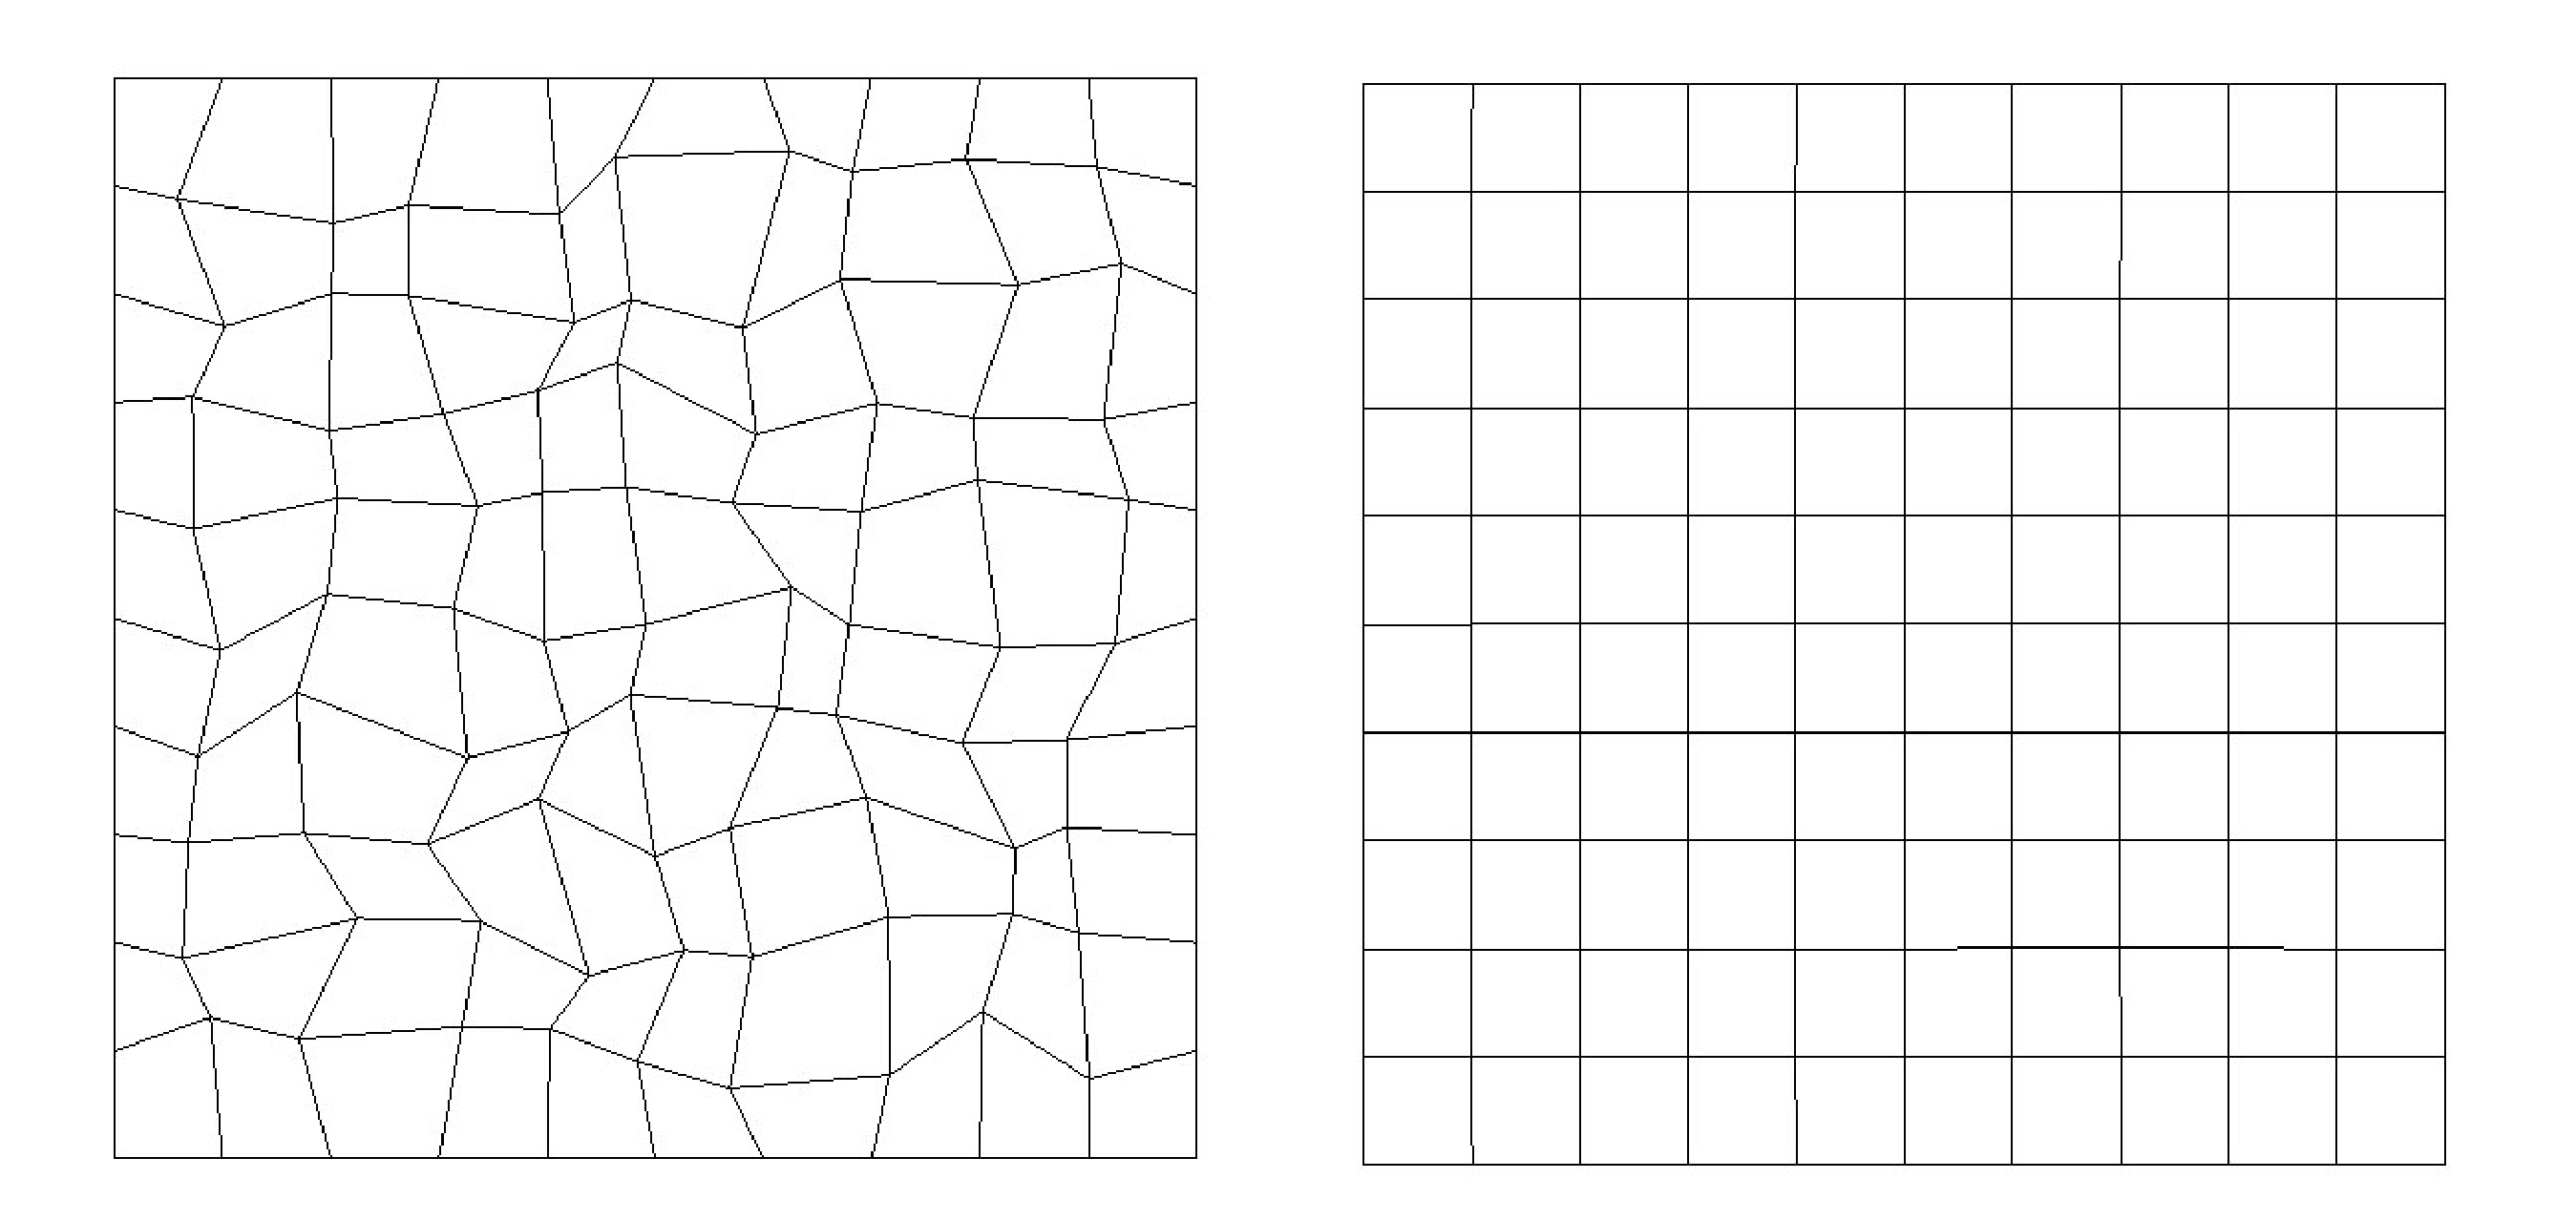
\includegraphics[height=80mm]{square_rand.eps}
    \caption{square\_quad\_10\_rand.vtk mesh. The original mesh is on the left, the mesh smoothed with the \texttt{LaplacianSmoother} is shown on the right.}
    \label{fig:square_rand}
\end{center}
\end{figure*}


\subsection{Improving the Mesh with the Low Level API}
\label{sec:tutDetailedAPI}
If the user requires in-depth control over the mesh quality improvement
process, the use of lower-level Mesquite classes provides an extensive
amount of flexibility.   In particular, the user can specify the quality
metric, objective function template, and optimization algorithm by
instantiating particular instances of each.  For each, various options
such as numerical or analytical gradient and Hessian evaluations or
the patch size can be selected.  Furthermore, the user can fine tune
the optimization algorithm performance by creating and setting the parameters 
of the termination criteria.
%for both inner and outer iterations.
%mbrewer removed reference to inner and outer iterations.
%{\tt LAF have we talked about inner and outer iterations before? perhaps
%too advanced for the tutorial}

Once these core objects have been created and customized, the user
creates an instruction queue and adds one or more quality improvers
and quality assessors to it.  The mesh optimization process is initiated
with the {\tt run\_instructions} method on the instruction queue
class.

In this section, we provide a simple example to highlight the main
steps needed for this approach.  The code segment given below performs
the same functionality as the wrapper class highlighted in the
previous section.  The comment lines provide high level documentation;
the details of each class and the low-level API are not described here.
%extensively treated in Section 
%\ref{sec:detailedAPI}.

\begin{verbatim}
    // creates a mean ratio quality metric ...
  IdealWeightInverseMeanRatio inverse_mean_ratio(err);

    // sets the objective function template
  LPtoPTemplate obj_func(&inverse_mean_ratio, 2, err);
  
    // creates the optimization procedures
  TrustRegion t_region(&obj_func);

    //performs optimization globally
  t_region.use_global_patch(); 

    // creates a termination criterion and 
    // add it to the optimization procedure
    // outer loop: default behavior: 1 iteration
    // inner loop: stop if gradient norm < eps
  TerminationCriterion tc_inner;
  tc_inner.add_absolute_gradient_L2_norm( 1e-4 ); 
  t_region.set_inner_termination_criterion(&tc_inner);

    // creates a quality assessor
  QualityAssessor m_ratio_qa(&inverse_mean_ratio);
    // creates an instruction queue
  InstructionQueue queue;
  queue.add_quality_assessor(&m_ratio_qa, err); 
  queue.set_master_quality_improver(&t_region, err); 
  queue.add_quality_assessor(&m_ratio_qa, err); 

    // do optimization of the mesh_set
  MeshDomainAssoc mesh_and_domain = MeshDomainAssoc(&my_mesh, &my_mesh_plane);
  queue.run_instructions(&mesh_and_domain, err);
  if (err) {
    std::cout << err << std::endl;
    return 2;
  }
\end{verbatim} 

\newpage

\subsection{Mesh Improvement Examples}

The left image in figure \ref{fig:hole} shows a mesh that has
been degraded by moving the disk from the right side of the square to
the left while keeping the mesh topology fixed.
The mesh file
\newline
\texttt{mesquite/meshFiles/2D/VTK/hole\_in\_square.vtk} contains the
information for this mesh.  If you plan to run this example, note that
the normal direction that defines the geometry is now $(0,0,-1)$.
This change must be made in the tutorial example code
as was done in section \ref{sec:tutMesh}, or an error message will be
thrown.
\begin{verbatim}
  Vector3D normal(0,0,-1);
  Vector3D point(0,0,-5);
  PlanarDomain my_mesh_plane(normal, point);
\end{verbatim}

We can now improve the mesh with the wrapper mentioned in
\ref{sec:tutWrapper} or the detailed API mentioned in
\ref{sec:tutDetailedAPI}. 
Because we changed the normal, the driver code must be recompiled;
otherwise the code and executable are as before.
Once the code is recompiled, type 
\begin{verbatim}
./tutorial ../../meshFiles/2D/VTK/hole_in_square.vtk
\end{verbatim}
to improve this mesh.
The smoothed mesh is shown in the right image of figure
\ref{fig:hole}.
The vertex locations have been repositioned and significantly improve
the quality of the mesh, as shown by the onscreen
quality assessor output:  
\begin{verbatim}
************** QualityAssessor(free only) Summary **************

  Evaluating quality for 140 elements.
  This mesh had 140 quadrilateral elements.
  There were no inverted elements detected.
  No entities had undefined values for any computed metric.

     Element Quality Statistics

     minimum     average         rms     maximum    std.dev.
     1.07588     85.8391     463.357     5037.46     455.336

     Number of statistics = 140
     Metric = Inverse Mean Ratio
     Element Quality not based on sample points.


************** QualityAssessor(free only) Summary **************

  Evaluating quality for 140 elements.
  This mesh had 140 quadrilateral elements.
  There were no inverted elements detected.
  No entities had undefined values for any computed metric.

     Element Quality Statistics

     minimum     average         rms     maximum    std.dev.
     1.01896     1.83479     1.91775     3.36336    0.557969

     Number of statistics = 140
     Metric = Inverse Mean Ratio
     Element Quality not based on sample points
\end{verbatim}
\begin{figure*}[htbp]
\begin{center}
    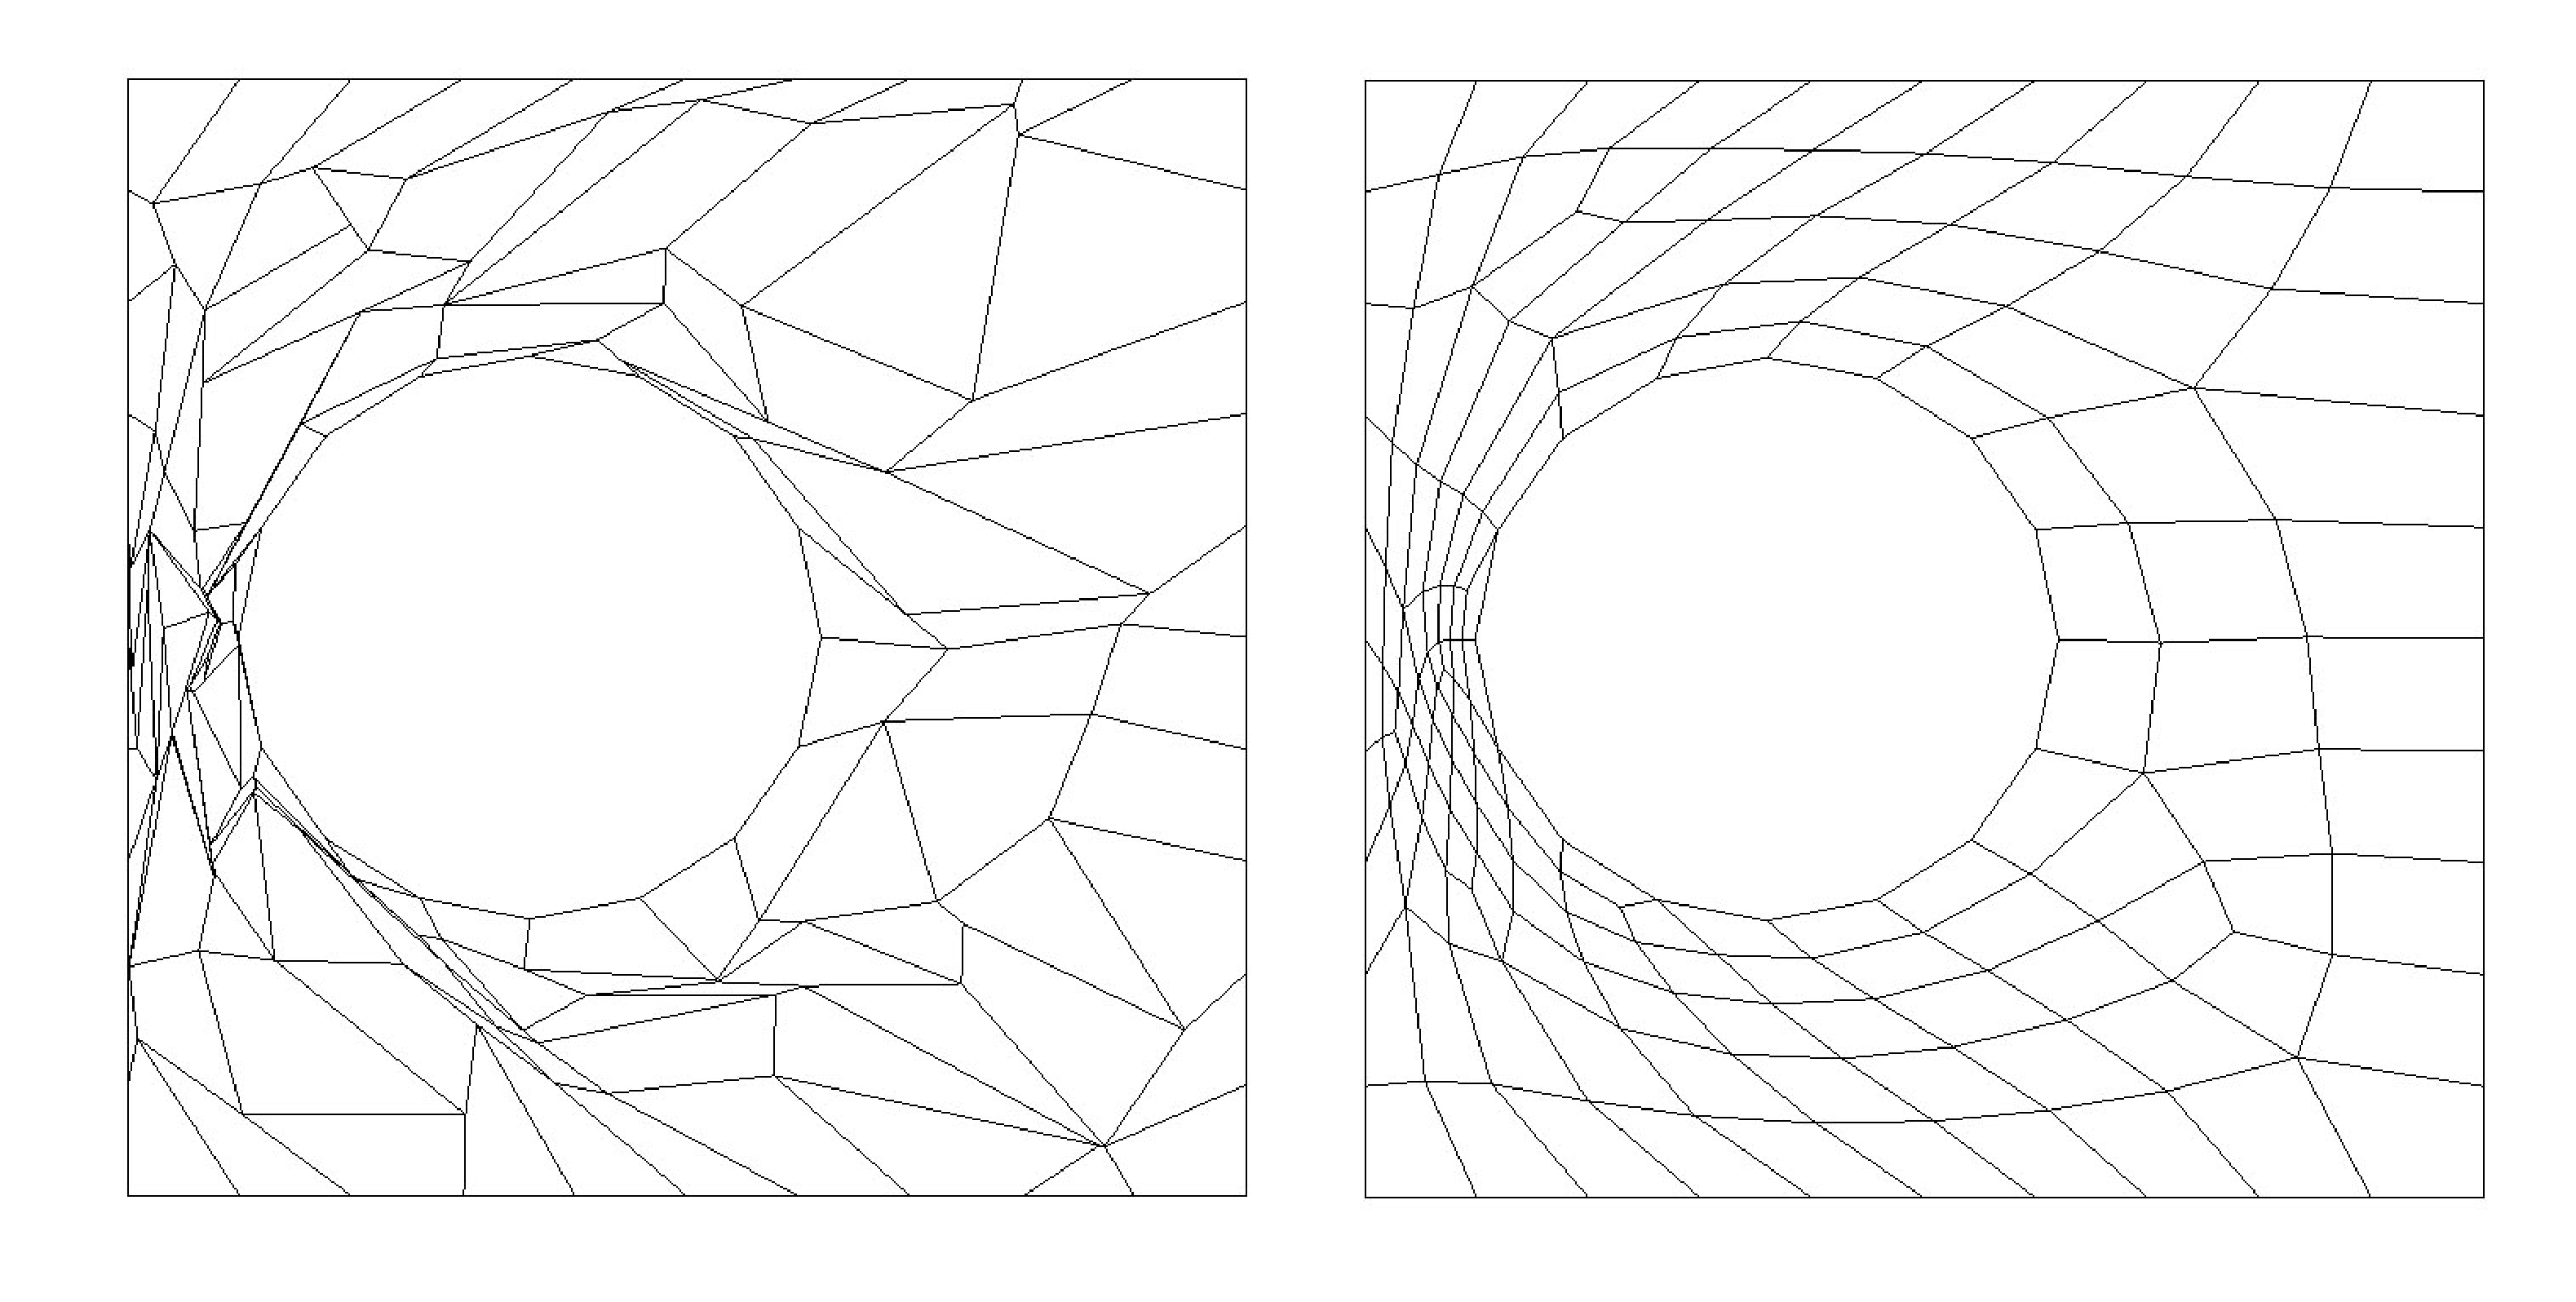
\includegraphics[height=80mm]{hole_in_square.eps}
    \caption{hole\_in\_square.vtk mesh. The original mesh is on the left, the mesh smoothed with
    Mesquite is shown on the right.}
    \label{fig:hole}
\end{center}
\end{figure*}


%%... section on testing ...

\subsection{Regression Testing}
\label{sec:RegressionTesting}
Regression testing encompasses
running unit tests as well as comparing results data against "blessed"
or "gold" data.  An example of comparing results of a smoothed mesh
against a gold version is in
\texttt{mesquite/testSuite/parallel\_smooth\_laplace/par\_hex\_smooth\_laplace.cpp}.
This utilizes a function in \texttt{MeshUtil}, \texttt{meshes\_are\_different}, to compare
two \texttt{MeshImpl} objects (within a specified numerical tolerance).  It is
recommended that both unit testing and gold-comparison testing be
included in your test code development.


% Getting Mesh Into Mesqite
\chapter{Getting Mesh Into Mesquite}
\label{sec:meshes}

The application must provide Mesquite with data on which to operate.  The two
fundamental classes of information Mesquite requires are:
\begin{itemize}
\item Mesh vertex coordinates and element connectivity, and
\item Constraints on vertex movement.
\end{itemize}
In this chapter we will assume that the only constraint available for vertex movement is to flag the vertices as fixed.  More advanced constraints such as vertices following geometric curves or surfaces are discussed in the following chapter.  

The mesh data expected as input to Mesquite is a set of vertices and elements.  Each vertex has associated with it a fixed flag, a ``byte'', and x, y, and z coordinate values.  The fixed flag is used as input only.  It indicates whether or not the corresponding vertex position should be fixed (i.e., coordinates not allowed to change) during the optimization.  The ``byte'' is one byte of Mesquite-specific working data associated with each vertex (currently only used for vertex culling.)   The coordinate values for each vertex serve as both input and output: as input they are the initial positions of the vertices and as output they are the optimized positions.  

Each element of the input mesh has associated with it a type and a list of vertices.  The type is one of the values defined in \texttt{Mesquite::EntityTopology} (\texttt{Mesquite.hpp}).  It species the topology (type of shape) of the element. Currently supported element types are triangles, quadrilaterals, 
tetrahedra, hexahedra, triangular wedges, and pyramids.  The list of vertices (commonly referred to as the ``connectivity'') define the geometry (location and variation of shape) for the element.  The vertices are expected to be in a pre-defined order specific to the element topology. Mesquite uses the canonical ordering defined in the ExodusII specification\cite{exodus}.

For some more advanced capabilities, Mesquite may require the ability to attach arbitrary pieces of data (called ``tags'') to mesh elements or vertices. For more on tags see Section \ref{sec:tags_section}.


\section{The \texttt{Mesquite::Mesh} Interface} \label{sec:MeshData}

The \texttt{Mesquite::Mesh} class (\texttt{MeshInterface.hpp}) defines the interface Mesquite uses to interact with mesh data.  In C++ this means that the class defines a variety of pure virtual (or abstract) functions for accessing mesh data.  An application may implement a subclass of \texttt{Mesquite::Mesh}, providing implementations of the virtual methods that allow Mesquite direct access to the applications in-memory mesh representation.  

The \texttt{Mesquite::Mesh} interface defines functions for operations such as:
\begin{itemize}
\item Get a list of all mesh vertices.
\item Get a list of all mesh elements.
\item Get a property of a vertex (coordinates, fixed flag, etc.)
\item Set a property of a vertex (coordinates, ``byte'', etc.)
\item Get the type of an element
\item Get the vertices in an element
\end{itemize}
It also defines other operations that are only used for certain optimization algorithms:
\begin{itemize}
\item Get the list of elements for which a specific vertex occurs in the connectivity list.
\item Define a ``tag'' and use it to associate data with vertices or elements.
\end{itemize}

Mesh entities (vertices and elements) are referenced in the \texttt{Mesquite::Mesh} interface using `handles'.  There must be a unique handle
space for all vertices, and a separate unique handle space for all elements. 
That is, there must be a one-to-one mapping between handle values and vertices,
and a one-to-one mapping between handle values and elements.  The storage type of
the handles is specified by 
\begin{center}
\texttt{Mesquite::Mesh::VertexHandle} and \texttt{Mesquite::Mesh::ElementHandle}.
\end{center}
The handle types are of sufficient size
to hold either a pointer or an index, allowing the underlying implementation of
the \texttt{Mesquite::Mesh} interface to be either pointer-based or index-based. 
All mesh entities are referenced using handles.  For example, the
\texttt{Mesquite::Mesh} interface declares a method to retrieve the list of all
vertices as an array of handles and a method to update the coordinates of a
vertex where the vertex is specified as a handle.

It is recommended that the application invoke the Mesquite optimizer for subsets
of the mesh rather than the entire mesh whenever it makes sense to do so.  For
example, if a mesh of two geometric volumes is to be optimized and all mesh
vertices lying on geometric surfaces are constrained to be fixed (such vertices
will not be moved during the optimization) then optimizing each volume separately
will produce the same result as optimizing both together.  


\section{Accessing Mesh In Arrays} \label{sec::ArrayMesh}

One common representation of mesh in applications is composed of simple 
coordinate and index arrays.  Mesquite provides the \texttt{ArrayMesh} implementation of the \texttt{Mesquite::Mesh} interface to allow Mesquite
to access such array-based mesh definitions directly.  The mesh must be
defined as follows:
\begin{itemize}
\item Vertex coordinates must be stored in an array of double-precision
      floating-point values.  The coordinate values must be interleaved,
      meaning that the x, y, and z coordinate values for a single vertex
      are contiguous in memory.
\item The mesh must be composed of a single element type.
\item The element connectivity (vertices in each element) must be stored
      in an interleaved format as an array of long integers.  The vertices
      in each element are specified by an integer \texttt{i}, where the location       of the coordinates of the corresponding vertex is located at position
      \texttt{3*i} in the vertex coordinates array.
\item The fixed/boundary state of the vertices must be stored in an array
      of integer values, where a value of 1 indicates a fixed vertex and a 
      value of 0 indicates a free vertex.  The values in this array must
      be in the same order as the corresponding vertex coordinates in the
      coordinate array.
\end{itemize}

The following is a simple example of using the ArrayMesh object to pass
Mesquite a mesh containing four quadrilateral elements.
\begin{lstlisting}
/** define some mesh **/
    /* vertex coordinates */
  double coords[] = { 0, 0, 0,
                      1, 0, 0,
                      2, 0, 0,
                      0, 1, 0,
                     .5,.5, 0,
                      2, 1, 0,
                      0, 2, 0,
                      1, 2, 0,
                      2, 2, 0 };
    /* quadrilateral element connectivity (vertices) */
  long quads[] = { 0, 1, 4, 3,
                   1, 2, 5, 4,
                   3, 4, 7, 6,
                   4, 5, 8, 7 };
    /* all vertices except the center one are fixed */
  int fixed[] = { 1, 1, 1,
                  1, 0, 1,
                  1, 1, 1 };
  
/** create an ArrayMesh to pass the above mesh into Mesquite **/
  
  ArrayMesh mesh( 
      3,            /* 3D mesh (three coord values per vertex) */
      9,            /* nine vertices */
      coords,       /* the vertex coordinates */ 
      fixed,        /* the vertex fixed flags */
      4,            /* four elements */
      QUADRILATERAL,/* elements are quadrilaterals */
      quads );      /* element connectivity */
  
/** smooth the mesh **/
  
    /* Need surface to constrain 2D elements to */
  PlanarDomain domain( PlanarDomain::XY );

  MsqError err;
  ShapeImprover shape_wrapper;
  if (err) {
    std::cout << err << std::endl;
    exit (2);
  }
  
  shape_wrapper.run_instructions( &mesh, &domain, err );
  if (err) {
    std::cout << "Error smoothing mesh:" << std::endl
              << err << std::endl;
  }
  
/** Output the new location of the center vertex **/
  std::cout << "New vertex location: ( "
            << coords[12] << ", " 
            << coords[13] << ", " 
            << coords[14] << " )" << std::endl;
\end{lstlisting}

NOTE:  When using the \texttt{ArrayMesh} interface, the application is responsible for managing the storage of the mesh data.  The \texttt{ArrayMesh}
 does NOT copy the input mesh.  

 
\section{Reading Mesh From Files} \label{sec:meshFiles}

Mesquite provides a concrete implementation of the \texttt{Mesquite::Mesh} named
\texttt{Mesquite::MeshImpl}.  This implementation is capable of reading mesh from
VTK\cite{VTKbook, VTKuml} and optionally ExodusII files. See Sections 
\ref{sec:depends} and \ref{sec:compiling} for more 
information regarding the optional support for ExodusII files.

The `fixed' flag for vertices can be specified in VTK files by defining a
SCALAR POINT\_DATA attribute with values of 0 or 1, where 1 indicates that the
corresponding vertex is fixed.  The \texttt{Mesquite::MeshImpl} class is capable
of reading and storing tag data (see Section \ref{sec:tags_section}) using VTK attributes and
field data.  The current implementation writes version 3.0 of the VTK file format
and is capable of reading any version of the file format up to 3.0.  


\section{ITAPS iMesh Interface}

\subsection{Introduction}

The ITAPS Working Group has defined a standard API for exchange of mesh data between applications.  The iMesh interface\cite{imesh} defines a superset of the functionality required for the \texttt{Mesquite::Mesh} interface.  Mesquite can access mesh through an iMesh interface using the \texttt{Mesquite::MsqIMesh} class declared in \texttt{MsqIMesh.hpp}.  This class is an ``adaptor'':  it presents the iMesh interface as the \texttt{Mesquite::Mesh} interface.  

The primary advantage of this method of providing mesh data to mesquite is that it is designed for interoperability.  The same API can be used to provide other tools and services access to the mesh data.  And there are stand-alone mesh data base libraries that already implement this API such as MOAB\cite{MOAB-webpage} and FMDB\cite{FMDB-webpage}.  It is also possible to implement the iMesh interface in Fortran.

\subsection{Overview}

A \texttt{Mesquite::MsqIMesh} instance must be provided with at least two pieces of information: The \texttt{iMesh\_Instance} handle and an \texttt{iBase\_EntitySetHandle}.  The optional \texttt{iBase\_TagHandle} for the ``fixed tag'' must frequently be provided as well.  The \texttt{iMesh\_Instance} specifies the instance of the database containing the mesh.  The \texttt{iBase\_EntitySetHandle} handle specifies the subset of that mesh that is to be optimized by Mesquite.  If the entire mesh is to be optimized then the ``root set'' should be specified for this argument.  The quality of all elements in this set will be used to drive the mesh optimization.  All vertices adjacent to any elements in the set will be moved as a part of the optimization unless they are explicitly designated as fixed.  The ``fixed tag'' is used to indicate such vertices.  Every vertex adjacent to the input elements should be tagged with a single integer value of either zero or one for the ``fixed tag''.  A value of one indicates that the vertex is fixed while a value of zero indicates that the vertex location is to be optimized by Mesquite.

The boundary of the mesh must always be constrained in some way for the mesh optimization to produce valid results.  For a volume mesh this can be accomplished by either designating the vertices on the mesh boundary as fixed or by specifying a geometric domain (e.g. surfaces, curves, etc) that the boundary vertices are constrained to lie on.  For a surface mesh some geometric domain must always be specified (e.g. a surface) and it is still necessary to specify which vertices are fixed unless the geometric domain also includes the bounding geometric curves constraining the movement of the boundary mesh vertices\footnote{A surface mesh that forms a topological sphere has no boundary and therefore need not have vertices designated as fixed or otherwise constrained as long as the entire geometric domain is continuous.}.  Geometric domains are the topic of Chapter \ref{sec:geom}.  Further discussion and examples in this section will be limited to volume meshes and true 2D meshes, both with the boundary vertices designated as fixed via the ``fixed tag''. 

Designating vertices as fixed is the responsibility of the application using Mesquite.  This responsibility is left to the application (as opposed to providing some utility in Mesquite to find the ``skin'' of a mesh) for several reasons.  An application can often obtain the set of vertices bounding a region of mesh directly through data not available to Mesquite.  For example if the application has a B-rep solid model for which the mesh is a discretization then it typically can obtain the bounding vertices as the set of vertices associated with the bounding geometric entities.  Further, there exist cases where the fixed vertices are more than just those on the topological boundary of the mesh.  For example, consider the mesh of a conic surface that includes a vertex at the apex of the cone.  Such a vertex must be designated as fixed because the lack of a valid surface normal at that point will interfere with the correct functioning of Mesquite.  Such a vertex cannot be reliably identified given only the mesh.  However, identifying such vertices typically happens naturally when obtaining the set of fixed vertices from the association with bounding geometric entities.  Finally, the optimal implementation of a ``skinning'' operation depends greatly on details of the mesh representation that Mesquite is not aware of and is not otherwise concerned with.

\subsection{Practical Details}

The \texttt{Mesquite::MsqIMesh} class caches data related to the input \texttt{iBase\_EntitySetHandle} upon construction.  If the contents of the referenced entity set change, or the vertices associated with elements contained in that set change, then the application should either re-create the \texttt{Mesquite::MsqIMesh} instance or notify an existing instance of the change by calling the \texttt{set\_active\_set} member function.  Similarly, while the implementation does not at the time of this writing cache data related to the ``fixed tag'', it may do so in the future.  For forward compatibility the application should consider calling the \texttt{set\_fixed\_tag} method of \texttt{Mesquite::MsqIMesh} to notify the instance that the value of the tag may have changed for some mesh vertices.

The current version of Mesquite uses the following functions from the iMesh interface:
\begin{itemize}
\item \texttt{iMesh\_getRootSet}
\item \texttt{iMesh\_getGeometricDimension}
\item \texttt{iMesh\_getEntities}
\item \texttt{iMesh\_getNumOfType}
\item \texttt{iMesh\_isEntContained}
\item \texttt{iMesh\_getEntArrTopo}
\item \texttt{iMesh\_getEntArrAdj}
\item \texttt{iMesh\_getVtxArrCoords}
\item \texttt{iMesh\_setVtxCoord}
\item \texttt{iMesh\_createTag}
\item \texttt{iMesh\_destroyTag}
\item \texttt{iMesh\_getTagName}
\item \texttt{iMesh\_getTagSizeBytes}
\item \texttt{iMesh\_getTagType}
\item \texttt{iMesh\_getTagHandle}
\item \texttt{iMesh\_getIntArrData}
\item \texttt{iMesh\_getIntData}
\item \texttt{iMesh\_getArrData}
\item \texttt{iMesh\_setArrData}
\item \texttt{iMesh\_setIntData}
\item \texttt{iMesh\_setIntArrData}
\end{itemize}

An implementation should provide complete implementations of all of these methods to guarantee compatibility with all possible Mesquite algorithms. 

\subsection{Volume Example}

The following example demonstrates the use of the \texttt{ShapeImprover} wrapper with an implementation of the iMesh interface.  It is assumed that the application has implemented the iMesh interface to provide access to its own data or is using an existing implementation of the iMesh interface to store its mesh data.  The example illustrates the setup necessary to correctly pass a subset of a mesh to mesquite and how to designate boundary vertices as fixed using the ``fixed tag''.  The input to the example function is the \texttt{iMesh\_Instance} handle and an \texttt{iBase\_EntitySetHandle} specifying both the elements for which to improve the quality and the free vertices.  The example code uses this application-supplied designation of which vertices are fixed to initialize the ``fixed tag''.

\begin{lstlisting}

#include <MsqError.hpp>
#include <ShapeImprover.hpp>
#include <MsqIMesh.hpp>
#include <vector>
#include <iostream>
#include <iMesh.h>

using namespace Mesquite;

/**\brief Call Mesquite ShapeImprovement wrapper for volume mesh
 *
 * Smooth mesh accessed through ITAPS APIs using Mesquite
 * ShapeImprover.
 *
 *\param mesh_instance iMesh API instance
 *\param mesh A set defined in 'mesh_instance' that contains
 *            *both* the set of elements to smooth *and* the
 *            set of interior vertices that are to be moved
 *            to improve the quality of the mesh.  This set
 *            must *not* contain vertices on the boundary of
 *            the volume mesh.
 *\return mesquite error code or imesh error code
 *        (0 for success in all cases.)
 */
int shape_improve_volume( iMesh_Instance mesh_instance,
                          iBase_EntitySetHandle mesh )
{
  MsqPrintError err(std::cerr);
  int ierr;
  iBase_EntityHandle *ptr1, *ptr2;
  int *ptr3, *ptr4;
  int i5, i6, i7, i8, i9, i10, i11;
  \<const int elem_dim = 3;\>
  \<const int max_vtx_per_elem = 8;\>
  
    // create adapter (should also create fixed tag)
  MsqIMesh mesh_adapter( mesh_instance, mesh, elem_dim, err );
  if (err) return err.error_code();

    // get tag for marking vertices as fixed
    // Note: we assume here that the tag has already been created.
  iBase_TagHandle fixed_tag = 0;
  iMesh_getTagHandle( mesh_instance,
                      "fixed",
                      &fixed_tag,
                      &ierr,
                      strlen("fixed") );
  if (iBase_SUCCESS != ierr) return ierr;

    // get all vertices in mesh
  int count, num_vtx;
  iMesh_getNumOfType( mesh_instance, mesh, elem_dim, &count, &ierr );
  if (iBase_SUCCESS != ierr) return ierr;
  std::vector<iBase_EntityHandle> elems(count), verts(max_vtx_per_elem*count);
  std::vector<int> indices(max_vtx_per_elem*count), offsets(count+1);
  ptr1 = &elems[0];
  ptr2 = &verts[0];
  ptr3 = &indices[0];
  ptr4 = &offsets[0];
  i5 = elems.size();
  i7 = verts.size();
  i8 = indices.size();
  i10 = offsets.size();
  iMesh_getAdjEntIndices( mesh_instance, mesh, 
                          elem_dim, iMesh_ALL_TOPOLOGIES, iBase_VERTEX,
                          &ptr1, &i5, &i6,
                          &ptr2, &i7, &num_vtx,
                          &ptr3, &i8, &i9,
                          &ptr4, &i10, &i11, &ierr );
  if (iBase_SUCCESS != ierr) return ierr;
  verts.resize( num_vtx );

    // set fixed flag on all vertices
  std::vector<int> tag_data(num_vtx, 1);
  iMesh_setIntArrData( mesh_instance, &verts[0], verts.size(), 
                       fixed_tag, &tag_data[0], tag_data.size(), &ierr );
  if (iBase_SUCCESS != ierr) return ierr;

    // clear fixed flag for vertices contained directly in set
  iMesh_getNumOfType( mesh_instance, mesh, iBase_VERTEX, &count, &ierr );
  if (iBase_SUCCESS != ierr) return ierr;
  verts.resize( count );
  ptr1 = &verts[0];
  i5 = verts.size();
  iMesh_getEntities( mesh_instance, mesh, iBase_VERTEX, iMesh_ALL_TOPOLOGIES,
                     &ptr1, &i5, &i6, &ierr );
  if (iBase_SUCCESS != ierr) return ierr;
  tag_data.clear();
  tag_data.resize( verts.size(), 0 );
  iMesh_setIntArrData( mesh_instance, &verts[0], verts.size(), 
                       fixed_tag, &tag_data[0], tag_data.size(), &ierr );
  if (iBase_SUCCESS != ierr) return ierr;

    // Finally, smooth the mesh
  ShapeImprover smoother;
  \<smoother.run_instructions( &mesh_adapter, err );\>
  if (err) return err.error_code();

  return 0;
}
\end{lstlisting}

\subsection{Two-dimensional Example}

This section presents an example of how to use Mesquite to optimize a 2D mesh.  It is a modification of the example from the previous section with changes shown in blue.  As Mesquite operates only on 3D meshes (either volume or surface), a 2D mesh is optimized by treating it as a surface mesh constrained to the XY plane.


\begin{lstlisting}

#include <MsqError.hpp>
#include <ShapeImprover.hpp>
#include <MsqIMesh.hpp>
\<#include <PlanarDomain.hpp>\>
#include <vector>
#include <iostream>
#include <iMesh.h>

using namespace Mesquite;

/**\brief Call Mesquite ShapeImprovement wrapper for 2D mesh
 *
 * Smooth mesh accessed through ITAPS APIs using Mesquite
 * ShapeImprover.
 *
 *\param mesh_instance iMesh API instance
 *\param mesh A set defined in 'mesh_instance' that contains
 *            *both* the set of elements to smooth *and* the
 *            set of interior vertices that are to be moved
 *            to improve the quality of the mesh.  This set
 *            must *not* contain vertices on the boundary of
 *            the mesh.
 *\return mesquite error code or imesh error code
 *        (0 for success in all cases.)
 */
int shape_improve_2D( iMesh_Instance mesh_instance,
                      iBase_EntitySetHandle mesh )
{
  MsqPrintError err(std::cerr);
  int ierr;
  iBase_EntityHandle *ptr1, *ptr2;
  int *ptr3, *ptr4;
  int i5, i6, i7, i8, i9, i10, i11;
  \<const int elem_dim = 2;\>
  \<const int max_vertex_per_elem = 4;\>
  
    // create adapter (should also create fixed tag)
  MsqIMesh mesh_adapter( mesh_instance, mesh, elem_dim, err );
  if (err) return err.error_code();

    // get tag for marking vertices as fixed
    // Note: we assume here that the tag has already been created.
  iBase_TagHandle fixed_tag = 0;
  iMesh_getTagHandle( mesh_instance,
                      "fixed",
                      &fixed_tag,
                      &ierr,
                      strlen("fixed") );
  if (iBase_SUCCESS != ierr) return ierr;

    // get all vertices in mesh
  int count, num_vtx;
  iMesh_getNumOfType( mesh_instance, mesh, elem_dim, &count, &ierr );
  if (iBase_SUCCESS != ierr) return ierr;
  std::vector<iBase_EntityHandle> elems(count), verts(max_vtx_per_elem*count);
  std::vector<int> indices(max_vtx_per_elem*count), offsets(count+1);
  ptr1 = &elems[0];
  ptr2 = &verts[0];
  ptr3 = &indices[0];
  ptr4 = &offsets[0];
  i5 = elems.size();
  i7 = verts.size();
  i8 = indices.size();
  i10 = offsets.size();
  iMesh_getAdjEntIndices( mesh_instance, mesh, 
                          elem_dim, iMesh_ALL_TOPOLOGIES, iBase_VERTEX,
                          &ptr1, &i5, &i6,
                          &ptr2, &i7, &num_vtx,
                          &ptr3, &i8, &i9,
                          &ptr4, &i10, &i11, &ierr );
  if (iBase_SUCCESS != ierr) return ierr;
  verts.resize( num_vtx );

    // set fixed flag on all vertices
  std::vector<int> tag_data(num_vtx, 1);
  iMesh_setIntArrData( mesh_instance, &verts[0], verts.size(), 
                       fixed_tag, &tag_data[0], tag_data.size(), &ierr );
  if (iBase_SUCCESS != ierr) return ierr;

    // clear fixed flag for vertices contained directly in set
  iMesh_getNumOfType( mesh_instance, mesh, iBase_VERTEX, &count, &ierr );
  if (iBase_SUCCESS != ierr) return ierr;
  verts.resize( count );
  ptr1 = &verts[0];
  i5 = verts.size();
  iMesh_getEntities( mesh_instance, mesh, iBase_VERTEX, iMesh_ALL_TOPOLOGIES,
                     &ptr1, &i5, &i6, &ierr );
  if (iBase_SUCCESS != ierr) return ierr;
  tag_data.clear();
  tag_data.resize( verts.size(), 0 );
  iMesh_setIntArrData( mesh_instance, &verts[0], verts.size(), 
                       fixed_tag, &tag_data[0], tag_data.size(), &ierr );
  if (iBase_SUCCESS != ierr) return ierr;

    // Finally, smooth the mesh
  ShapeImprover smoother;
  \<PlanarDomain xyplane(PlanarDomain::XY);\>
  \<smoother.run_instructions( &mesh_adapter, &xyplane, err );\>
  if (err) return err.error_code();

  return 0;
}
\end{lstlisting}

\section{Tags} \label{sec:tags_section}

\subsection{Using Tags}

Mesquite has the ability to attach arbitrary pieces of data to mesh elements or vertices via the use of tags.  Assigning tag data to a vertex or element is a two step process.  First, the tag itself is created to describe the tag name, type, and size.  Second, the actual data value is associated with the vertex or element using the tag as a descriptor.

When a tag itself is created, it is given a name and associated data type.  Valid Mesquite Tag Types are: BYTE, BOOL, INT, DOUBLE, and HANDLE. Tags are created using the method MeshImpl::tag\_create() or one of it derived forms.

Mesquite can also handle VTK tags.  Valid VTK Tag Types are: SCALAR, COLOR, VECTOR, NORMAL, TEXTURE, TENSOR, and FIELD. VTK tags and data are assigned as part of the reading a VTK file operation and can be created and manipulated from within Mesquite.  The VTK tags and data are persistent for the VTK entitles within Mesquite including when they are written back to a file.

Once the tag is created, it is used to associate data to a vertex or element mesh entity using the methods MeshImpl::tag\_set\_vertex\_data() or MeshImpl::tag\_set\_element\_data().  Tagged data is recovered via MeshImpl::tag\_get\_vertex\_data() or MeshImpl::tag\_get\_element\_data().


\subsection{Vector Example}

The following is a simple example of using tags to associate vectors with elements of a mesh. It creates a simple mesh of two quads then creates a single tag consisting of 3 doubles to represent the vector. After creating the values for the two vectors, it associates the vectors with the elements of the mesh via a call to tag\_set\_element\_data().

\begin{lstlisting}
#include "Mesquite.hpp"
#include "MeshImpl.hpp"
#include "MsqError.hpp"

int main(int argc, char* argv[])
{

  const double vertices[] = { 0, 0, 0,
                              0, 1, 0,
                              1, 0, 0,
                              1, 1, 0,
                              2, 1, 0,
                              2, 0, 0};
  const int conn[] = {0, 1, 3, 2, 1, 5, 4, 3 };

  bool fixed[] = {true, true, true, true, true, true};
  Mesquite::MsqError err;
  std::vector<Mesquite::Mesh::ElementHandle>elements;

    // Create the mesh
  Mesquite::MeshImpl mesh(6, 2, Mesquite::QUADRILATERAL, fixed, vertices, conn);
  mesh.get_all_elements(elements, err);

  std::vector<double> v_tags(elements.size() * 3);

    // Create tag
  Mesquite::TagHandle v_tag = 
                mesh.tag_create("VECTOR", Mesquite::Mesh::DOUBLE, 3, NULL, err);

  std::vector<double> v_coords(6);
  v_coords[0] = 0.0;
  v_coords[1] = 0.0;
  v_coords[2] = -1.0;
  v_coords[3] = 0.0;
  v_coords[4] = 0.0;
  v_coords[5] = 1.0;

     // Associate vectors with elements
  mesh.tag_set_element_data(v_tag, elements.size(), 
                   mesquite::arrptr(elements), Mesquite::arrptr(v_coords) ,err);
  return 0;
}
\end{lstlisting}

\subsection{2x2 Matrix on vertices using Tags Example}

The follow code example shows another way tags can be used in Mesquite.  It attaches a 2x2 matrix to each vertex in a mesh by creating four tags and four arrays of doubles. The value for the matrices are stored in the arrays with each array representing one value of the matrix. Then the four tags are associated with the four arrays to create tagged data for each vertex representing the 2x2 matrix for it.


\begin{lstlisting}
int main(int argc, char* argv[])
{
  //  2 +-----+ 3
  //    |\    |
  //    | \   |
  //    |  \  |
  //    |   \ |
  //    |    \|
  //  0 +-----+ 1
 double tri_verts[] = { 0.0, 0.0, 0.0,
                        1.0, 0.0, 0.0,
                        0.0, 1.0, 0.0,
                        1.0, 1.0, 0.0 };

  const int tri_elems[] = { 0, 1, 2,
                            3, 2, 1 };

  bool fixed[] = {true, true, true, true};
  Mesquite::MsqError err;
  std::vector<Mesquite::Mesh::ElementHandle>elements;

    // Create the mesh
  Mesquite::MeshImpl mesh(4, 2, Mesquite::TRIANGLE, fixed, tri_verts, tri_elems);
  mesh.get_all_elements(elements, err);

  std::vector<double> lid1(elements.size());
  std::vector<double> lid2(elements.size());
  std::vector<double> lid3(elements.size());
  std::vector<double> lid4(elements.size());

  double adTestOri[4] = {0.0,0.0,0.0,0.0};
  for (unsigned int i=0; i < elements.size(); i++)
  {
    /****************************************************************
     Compute eigenvectors and eigenvalues to be used to set the Target
     (actual steps left out for simplicity of example)
    ****************************************************************/

    if (adTestOri[1]*adTestOri[1]+adTestOri[3]*adTestOri[3] >
        adTestOri[0]*adTestOri[0]+adTestOri[2]*adTestOri[2])
          {
      lid1[i] = -adTestOri[1];
      lid2[i] = adTestOri[0];
      lid3[i] = -adTestOri[3];
      lid4[i] = adTestOri[2];
    }
    else
    {
      lid1[i] = adTestOri[0];
      lid2[i] = adTestOri[1];
      lid3[i] = adTestOri[2];
      lid4[i] = adTestOri[3];
    }
  }

  const char LOCAL_ID_NAME1[] = "LOCAL_ID1";
  const char LOCAL_ID_NAME2[] = "LOCAL_ID2";
  const char LOCAL_ID_NAME3[] = "LOCAL_ID3";
  const char LOCAL_ID_NAME4[] = "LOCAL_ID4";

    // Create tags
  Mesquite::TagHandle lid_tag1 =
        mesh.tag_create(LOCAL_ID_NAME1, Mesquite::Mesh::DOUBLE, 1, NULL, err);
  Mesquite::TagHandle lid_tag2 =
        mesh.tag_create(LOCAL_ID_NAME2, Mesquite::Mesh::DOUBLE, 1, NULL, err);
  Mesquite::TagHandle lid_tag3 =
        mesh.tag_create(LOCAL_ID_NAME3, Mesquite::Mesh::DOUBLE, 1, NULL, err);
  Mesquite::TagHandle lid_tag4 =
        mesh.tag_create(LOCAL_ID_NAME4, Mesquite::Mesh::DOUBLE, 1, NULL, err);
  size_t num_cells=(elements.size());

    // Associate arrays representing 2x2 matricies to verticies
  mesh.tag_set_vertex_data(
      lid_tag1,num_cells,Mesquite::arrptr(elements),Mesquite::arrptr(lid1),err);
  mesh.tag_set_vertex_data(
      lid_tag2,num_cells,Mesquite::arrptr(elements),Mesquite::arrptr(lid2),err);
  mesh.tag_set_vertex_data(
      lid_tag3,num_cells,Mesquite::arrptr(elements),Mesquite::arrptr(lid3),err);
  mesh.tag_set_vertex_data(
      lid_tag4,num_cells,Mesquite::arrptr(elements),Mesquite::arrptr(lid4),err);

  return 0;
\end{lstlisting}

\section{Slaved Verticies} \label{sec:slaved_vertices}

Mesquite supports three types of vertices: fixed, free, and slaved.  Fixed vertices cannot be moved by optimization routines, free vertices are eligible to be moved, and slaved vertices are handled in a specific manner as described in this section.

Slaved vertices are used primarily with a mesh that contains higher order elements.  They are typically vertices at edge or face centers as well as element centers.  In the cases where these higher order nodes cannot or should not be used in an optimization or quality metric evaluation, they are marked as slaved.  This allows the operations to proceed as if those nodes were not present in the mesh but the slaved nodes can still be moved to retain the proper spatial relationship with any free nodes that were moved by the optimization.

How vertices can be moved by optimization routines is controlled by two flags in the MeshImplData class: fixed and slaved.  When the fixed flag is false the vertex is considered to be free, true signifies a fixed vertex.  True for the slaved flag marks the vertex as slaved.  The combination of fixed=true and slaved=true is not valid and will result in failures during processing of the mesh containing the vertices.


There are three ways in Mesquite to mark vertices as slaved:

1. When reading in a mesh from a VTK file, a dataset attribute of 'slaved' can be used to define which of the points in the mesh are slaved.  The following VTK input file describes a very contrived mesh of a single quad with four fixed vertices at the corners and a slaved vertex at the mid-point of each edge.  In the input file, the first four points defined are the corners, the next for are the mid-point nodes.



\begin{verbatim}
# vtk DataFile Version 3.0
Mesquite Mesh
ASCII
DATASET UNSTRUCTURED_GRID
POINTS 8 double
0 0 0
1 0 0
1 1 0
0 1 0
0.5 0 0
1 0.5 0
0.5 1 0
0 0.5 0
CELLS 1 9
8 0 1 2 3 4 5 6 7
CELL_TYPES 1
23
POINT_DATA 8
SCALARS fixed int
LOOKUP_TABLE default
1
1
1
1
0
0
0
0
SCALARS GLOBAL_ID int 1
LOOKUP_TABLE default
1
2
3
4
5
6
7
8
SCALARS slaved int 1
LOOKUP_TABLE default
0
0
0
0
1
1
1
1
CELL_DATA 1
SCALARS GLOBAL_ID int 1
LOOKUP_TABLE default
1
\end{verbatim}


2. A vertex can be marked as slaved by calling the method

 \texttt{MeshImplData::slave\_vertex(size\_t index, bool flag, MsqError\& err)} with the parameter 'flag' being "true" to signify slaved, "false" for not slaved.

3. The VertexBoundarySlaver class can be inserted in the instruction queue before any optimization to determine which higher-order nodes are slaved as a function of their distance from the boundary of the mesh.  It will attempt to automatically mark vertices as slaved according to the input parameters 'depth' and 'max\_boundary\_domain\_dimension'.  'depth' is the number of elements inwards from the boundary for which all contained higher-order nodes will be free variables in the optimization.  Any vertex further from the boundary will be slaved.  A depth of zero will result in all higher-order nodes being slaved except free nodes on the boundary.  'max\_boundary\_domain\_dimension' specifies the definition of "boundary".  If greater than or equal to 4, then the set of all fixed vertices is assumed to be the boundary.  If less than four, then all vertices constrained to a domain with the specified number of fewer degrees of freedom (constrained to a geometric entity with an equal or smaller topological dimension) will be considered to be the boundary.  If not specified, the boundary will be assumed to be indicated by fixed vertices.

Assuming a mesh has already been created, the following code snippet calls the VertexBoundarySlaver class to determine which vertices are to be slaved:

\begin{lstlisting}
  unsigned depth = 1;
  unsigned boundary = 2;
  Settings settings;
  settings.set_slaved_ho_node_mode( Settings::SLAVE_CALCULATED );
  SlaveBoundaryVertices determine_slaved_verts( depth, boundary );
  determine_slaved_verts.loop_over_mesh( &mesh, &domain, &settings, err );
\end{lstlisting}



% Mesquite Features
\chapter{Mesquite Features}

  This chapter is summarizes various aspects of Mesquite that will be useful in understanding the topics that follow.

\section{Solvers}

Many of the quality improvers in Mesquite work by minimizing the value of an
objective function (see Section \ref{sec:ObjectiveFunction}), where the
objective function is a function of the mesh vertex coordinates. 
The term \emph{solver} is often used to refer to the portion of the code in
the concrete subclass of \texttt{VertexMover} that implements the inner loop
of the optimization for quality improvers that optimize an explicit 
objective-function based (the code that implements the function-minimization algorithm.)

The remainder of this section lists the solvers available in Mesquite along with a small code example for each showing how to invoke the solver.


\subsection{Relaxation Smoothers}

Note that the relaxation smoothers do NOT require an objective function.

\subsubsection{LaplacianSmoother} 

Implements the Laplacian smoothing for a patch with one free vertex.  It moves the free center vertex to the average of the neighboring vertices.

\textbf{Code Example:}

\begin{lstlisting}[frame=single]
int main(int argc, char* argv[])
{
  const char input_file[] = MESH_FILES_DIR "2D/VTK/square_quad_2.vtk";

    /* Read a VTK Mesh file */
  MsqPrintError err(cout);
  Mesquite::MeshImpl mesh;
  mesh.read_vtk( input_file, err);
  if (err) return 1;
  
    // creates an intruction queue
  InstructionQueue queue1;
  
    // creates a mean ratio quality metric ...
  ConditionNumberQualityMetric shape_metric;
  EdgeLengthQualityMetric lapl_met;
  lapl_met.set_averaging_method(QualityMetric::RMS);
 
    // creates the laplacian smoother  procedures
  LaplacianSmoother lapl1;
  QualityAssessor stop_qa=QualityAssessor(&shape_metric);
  stop_qa.add_quality_assessment(&lapl_met);
  
    //**************Set stopping criterion****************
  TerminationCriterion sc2;
  sc2.add_iteration_limit( 10 );
  if (err) return 1;
  lapl1.set_outer_termination_criterion(&sc2);
  
  queue1.add_quality_assessor(&stop_qa,err); 
  if (err) return 1;
  queue1.set_master_quality_improver(&lapl1, err); 
  if (err) return 1;
  queue1.add_quality_assessor(&stop_qa,err); 
  if (err) return 1;
 
  PlanarDomain plane(Vector3D(0,0,1), Vector3D(0,0,5));
  
    // launches optimization on mesh
  queue1.run_instructions(&mesh, &plane, err); 
  if (err) return 1;

  return 0;
}
\end{lstlisting}

\subsubsection{SmartLaplacianSmoother}

Does same as the Laplacian smoother, but doesn't invert elements.  Invoked same way as the LaplacianSmoother.  If initial mesh in non-inverted, the SmartLaplacianSmoother performs Laplace smoothing while trying not to invert the mesh.

\subsubsection{Randomize}

The randomize smoother moves a free vertex to a random location within a local patch.  This smoother is provided as a convenience to
those who wish to generate a poor quality mesh from an initial mesh in order to test another mesh improvement algorithm.

\textbf{Code Example:}

\begin{lstlisting}[frame=single]
int main( )
{
  Mesquite::MeshImpl mesh;
  MsqPrintError err(cout);
  mesh.read_vtk(VTK_2D_DIR "tangled_quad.vtk", err);
  if (err) return 1;
  
  // Set Domain Constraint
  Vector3D pnt(0,0,0);
  Vector3D s_norm(0,0,1);
  PlanarDomain msq_geom(s_norm, pnt);
                                                                              
    // creates an intruction queue
  InstructionQueue queue1;
  
  Randomize rand(.05);
  
  TerminationCriterion sc_rand;
  sc_rand.add_iteration_limit( 10 );
 
  rand.set_outer_termination_criterion(&sc_rand);
  
  queue1.set_master_quality_improver(&rand, err);
  if (err) return 1;

  queue1.run_instructions(&mesh, &msq_geom, err);
  if (err) return 1;
  
  return 0;
}
\end{lstlisting}


\subsection{OptSolvers}

\subsubsection{ConjugateGradient}

Optimizes the objective function using the Polack-Ribiere scheme.

\textbf{Code Example:}

\begin{lstlisting}[frame=single]
int main( )
{
  Mesquite::MeshImpl mesh;
  MsqPrintError err(cout);
  mesh.read_vtk(VTK_2D_DIR "tangled_quad.vtk", err);
  if (err) return 1;
  
    // Set Domain Constraint
  Vector3D pnt(0,0,0);
  Vector3D s_norm(0,0,1);
  PlanarDomain msq_geom(s_norm, pnt);
                                                                              
    // creates an intruction queue
  InstructionQueue queue1;
  
    // creates a mean ratio quality metric ...
  ConditionNumberQualityMetric shape_metric;
  UntangleBetaQualityMetric untangle(2);

  LInfTemplate obj_func(&untangle);

  if (err) return 1;
    // creates the steepest descent optimization procedures
  ConjugateGradient cg( &obj_func, err );
  if (err) return 1;
  
  QualityAssessor stop_qa=QualityAssessor(&shape_metric);
  QualityAssessor stop_qa2=QualityAssessor(&shape_metric);
   
  stop_qa.add_quality_assessment(&untangle);

  queue1.add_quality_assessor(&stop_qa,err); 
  if (err) return 1;
 
  queue1.set_master_quality_improver(&cg, err);
  if (err) return 1;
  queue1.add_quality_assessor(&stop_qa2,err);
  if (err) return 1;

  queue1.run_instructions(&mesh, &msq_geom, err);
  if (err) return 1;
  
  return 0;
}
\end{lstlisting}


\subsubsection{FeasibleNewton}
Implements the newton non-linear programming algorithm in order to move a free vertex to an optimal position given an ObjectiveFunction object and a QualityMetric object.  This implementation of Feasible Newton works well on volume meshes and on surfaces meshes using PlanarDomain that lie in the X-Y coordinate plane. It should not be used on non-planar surface meshes.

\textbf{Code Example:}

\begin{lstlisting}[frame=single]
int main()
{     
  MsqPrintError err(cout);
  Mesquite::MeshImpl mesh;
  mesh.read_vtk(MESH_FILES_DIR "3D/vtk/tets/untangled/3D/tire.vtk", err);
  if (err) return 1;
  
    // creates an intruction queue
  InstructionQueue queue1;

    // creates a mean ratio quality metric ...
  IdealWeightInverseMeanRatio mean(err);
  if (err) return 1;
  
  LPtoPTemplate obj_func(&mean, 1, err);
  if (err) return 1;
  
    // creates the optimization procedures
  FeasibleNewton fn( &obj_func );

    //perform optimization globally
  fn.use_global_patch();
  if (err) return 1;
  
  queue1.set_master_quality_improver(&fn, err); 
  if (err) return 1;

  queue1.run_instructions(&mesh, err); 
  if (err) return 1;
  
  return 0;
}
\end{lstlisting}


\subsubsection{SteepestDescent}
A very basic implementation of the steepest descent optimization algorithm.  It works on patches of any size but the step size is automatically computed and is not accessible through the interface. It is for testing purposes only. 

\textbf{Code Example:}

\begin{lstlisting}[frame=single]
int main()
{
  MsqPrintError err(std::cout);
  Mesquite::MeshImpl mesh;
  mesh.read_vtk(MESH_FILES_DIR "3D/vtk/hexes/untangled/hexes_4by2by2.vtk", err);
  
    // creates an instruction queue
  InstructionQueue queue1;
  
    // creates a mean ratio quality metric ...
  IdealWeightInverseMeanRatio mean_ratio(err);
  if (err) return 1;
  ConditionNumberQualityMetric cond_num;
  mean_ratio.set_averaging_method(QualityMetric::LINEAR);
  
    // ... and builds an objective function with it
  LPtoPTemplate obj_func(&mean_ratio, 2, err);
  if (err) return 1;

   // creates the steepest descent optimization procedures
  SteepestDescent sd( &obj_func );
  sd.use_global_patch();
  
  QualityAssessor stop_qa=QualityAssessor(&mean_ratio);
  if (err) return 1;
  stop_qa.add_quality_assessment(&cond_num);
  if (err) return 1;
    
   //**************Set stopping criterion****************
  TerminationCriterion tc2;
  tc2.add_iteration_limit( 1 );
  sd.set_inner_termination_criterion(&tc2);

  queue1.add_quality_assessor(&stop_qa,err);
  queue1.set_master_quality_improver(&sd, err); 
  if (err) return 1;
  queue1.add_quality_assessor(&stop_qa,err);
  if (err) return 1;

  mesh.write_vtk("original_mesh.vtk", err); 
  if (err) return 1;
  
  queue1.run_instructions(&mesh, err);
  if (err) return 1;
  

  return 0;
}
\end{lstlisting}


\subsubsection{QuasiNewton}
Port of Todd Munson's quasi-Newton solver to Mesquite.

\textbf{Code Example:}

\begin{lstlisting}[frame=single]
int main()
{
  MsqPrintError err(std::cout);
  Mesquite::MeshImpl mesh;
  mesh.read_vtk(MESH_FILES_DIR "3D/vtk/hexes/untangled/hexes_4by2by2.vtk", err);
  
    // creates an intruction queue
  InstructionQueue queue1;
  
    // creates a mean ratio quality metric ...
  IdealWeightInverseMeanRatio mean_ratio(err);
  if (err) return 1;
  EdgeLengthQualityMetric cond_num;
  mean_ratio.set_averaging_method(QualityMetric::LINEAR);
  
    // build an objective function
  LPtoPTemplate obj_func(&mean_ratio, 2, err);
  if (err) return 1;

  QuasiNewton qn( &obj_func );
  qn.use_global_patch();
  
  QualityAssessor stop_qa=QualityAssessor(&mean_ratio);
  if (err) return 1;
  stop_qa.add_quality_assessment(&cond_num);
  if (err) return 1;
    
   //**************Set stopping criterion****************
  TerminationCriterion tc2;
  tc2.add_iteration_limit( 1 );
  qn.set_inner_termination_criterion(&tc2);

  queue1.add_quality_assessor(&stop_qa,err);
  queue1.set_master_quality_improver(&qn, err); 
  if (err) return 1;
  queue1.add_quality_assessor(&stop_qa,err);
  if (err) return 1;

  queue1.run_instructions(&mesh, err);
  if (err) return 1;
  
  return 0;
}
\end{lstlisting}


\subsubsection{TrustRegion}
Port of Todd Munson's trust region solver to Mesquite.  The TrustRegion optimizer is invoked in the same way as in the previous QuasiNewton example.


\section{Objective Function}
\label{sec:ObjectiveFunction}

\subsection{Definition}

An objective function is a scalar function of all the vertex coordinates in the active mesh.  The mesh vertex locations are optimized so as to minimize the objective function value.  

The objective functions implemented in Mesquite can be divided into two general categories: template objective functions and composite objective functions.  Template objective functions have an associated \texttt{QualityMetric} instance and typically implement some kind of averaging scheme.  Composite objective functions modify the values of one or two other objective functions, such as scaling the value or summing two values.

Most solvers in Mesquite also require the gradient of the objective function (the partial derivatives of the objective function with respect to the coordinate values of the free vertices in the patch.)  

\label{sec:Hessian} Some quality improvers (currently \texttt{FeasibleNewton}) need to know the Hessian (second partial derivatives) of the objective function.  Only an \texttt{ObjectiveFunction} implementation capable of providing Hessian data may be used with such a solver.  Mesquite provides numerical approximation of objective function gradient values, and of quality metric gradient and Hessian values, but not objective function Hessian values.  Further, Mesquite is capable of working only with Hessians of objective functions that have sparse Hessian matrices.  The Hessian matrix may only contain non-zero terms for vertex pairs that share at least one element.  This limitation is explicit in the implementation of the \texttt{MsqHessian} class, and is implicit in other areas of the code (such as portions of the \texttt{ObjectiveFunction} interface relating to use in a BCD algorithm.)  Some \texttt{ObjectiveFunction} implementations such as \texttt{CompositeOFMultiply} (the product of two other objective function values) and \texttt{StdDevTemplate} have a dense Hessian and therefore cannot be used with solvers requiring a Hessian.

Objective Functions only work with the QualityMetric classes, they do not work with the TargetMetrics classes.

\subsection{Objective Function Implementations}
\label{sec:objfunc_impl}

The \texttt{ObjectiveFunctionTemplate} is a base class for those objective function implementations that are some kind of average of quality metric values.  The \texttt{ObjectiveFunctionTemplate} class provides the API for associating a \texttt{QualityMetric} with an objective function and it provides a common implementation for initializing coordinate descent optimizations.

The composite objective functions modify one or two existing objective functions (e.g. adding two together).  All composite \texttt{ObjectiveFunction}s support analytical gradients and coordinate descent optimization if the underlying \texttt{ObjectiveFunction}s do.  Similarly, all except \texttt{CompositeOFMultiply} support analytical Hessians as long as their underlying \texttt{ObjectiveFunction}s do.  \texttt{CompositeOFMultiply} does not have a suitably sparse Hessian.

Two of the most commonly used objective functions are:

\begin{description}
\item[LPtoPTemplate] - Calculates the L\_p objective function raised to the pth power.
    That is, it sums the p-th powers of (the absolute value of) the quality metric values.

\item[PMeanPTemplate] - This class implements an objective function that is the power-mean
    of the quality metric evaluations raised to the power-mean power.  That is, the sum of 
   each quality metric value raised to a power, divided by the total number of quality 
   metric values.
\end{description}

\subsection{Example}

Below is a simplified version of the ShapeImprover Wrapper that has been annotated to illustrate the use of an objective function.

\begin{lstlisting}[frame=single]

void ShapeImprover::run_wrapper( Mesh* mesh,
                                ParallelMesh* pmesh,
                                MeshDomain* domain,
                                Settings* settings,
                                QualityAssessor* qa,
                                MsqError& err )
{
    // Quality Metrics

    // Used to obtain a target matrix for the quality assessment. Creates a
    // target matrix based on the element type and its ideal shape
  IdealShapeTarget target;

    // Local sample point quality metric is TShapeB1, a shape metric 
    // with barrier
  TShapeB1 mu;

    // A quality metric defined using 2D and 3D target metrics, where 
    // the active matrix compared to the target by the underlying 
    // metrics is the Jacobian matrix of the mapping function at a 
    // given sample point. Evaluates the quality metric at the sample
    // point by forming T in terms of the active and target matrices.
  TQualityMetric metric_0( &target, &mu );

    // A composite metric that converts the sample-based metric 
    // (metric_0) to an element-based metric by averaging the metric
    //  values at each sample point within the element
  ElementPMeanP metric( 1.0, &metric_0 );

    // QualityAssessor
  qa->add_quality_assessment( &metric );
    
    // an objective function that is the power-mean of the 
    // quality metric evaluations raised to the power-mean power.
  PMeanPTemplate obj_func( 1.0, &metric );

    // Optimizes the objective function using the Polack-Ribiere scheme.
  ConjugateGradient improver( &obj_func );

    // Treat the mesh as a single patch
  improver.use_global_patch();
  TerminationCriterion inner;
  inner.add_absolute_vertex_movement_edge_length( 0.005 );
  improver.set_inner_termination_criterion( &inner );
  InstructionQueue q;
  q.set_master_quality_improver( &improver, err ); MSQ_ERRRTN(err);
  q.add_quality_assessor( qa, err ); MSQ_ERRRTN(err);
  q.run_common( mesh, pmesh, domain, settings, err ); MSQ_ERRRTN(err);
}

\end{lstlisting}

In the above example, the quality metric TShapB1 can be replaced by any of the many quality metrics that are derived from the TMetric class.

\section{\texttt{MsqError}}
\label{sec:MsqError}

Almost every function in the Mesquite API accepts an instance of the \texttt{MsqError} class and uses that instance to flag the occurance of any errors.  For brevity, this argument is not shown or discussed for any function in the API.  The reader may assume an implicit final argument of type \texttt{MsqError\&} for almost every function shown or discussed in this document, the exceptions being those functions that cannot fail.

The \texttt{MsqError} class can be treated as a Boolean, where a true state indicates an error.  It can also be sent to a C++ output stream to print the error code, error message, and call stack (trace of nested function calls beginning with the topmost API call down to the function at which the error occured.)  An application will typically use an \texttt{MsqError} as follows:
\begin{lstlisting}
if (err) {
  std::cout << err << std::endl;
  return FAILURE;
}
\end{lstlisting}
The \texttt{MsqError} class also provides functions to progamatically extract data from such as the error message, error code, and call stack lines.

Mesquite also provides several macros to assist developers in using the \texttt{MsqError} class within Mesquite.  The \texttt{MSQ\_SETERR} macro is used to flag an initial error condition.  The following examples show typical uses of this macro:
\begin{lstlisting}
  // literal error message and error code
MSQ_SETERR(err)( "My error message", MsqError::UNKNOWN_ERROR );
  // error code and printf-style formatted error message
MSQ_SETERR(err)( MsqError::INVALID_ARG, "Argument 'foo' = %d", foo );
  // error code and default message for that error code
MSQ_SETERR(err)( MsqError::OUT_OF_MEMORY );
\end{lstlisting}

The \texttt{MSQ\_CHKERR} macro evalutes to true if an error has been flagged, and false otherwise.  Further, if an error has been flagged, it appends the location of the \texttt{MSQ\_CHKERR} invokation to the call stack maintained in the \texttt{MsqError} instance.  This is the mechanism by which Mesquite generates the call-stack data.  The following is an example of how this macro is typically used:
\begin{lstlisting}
  if (MSQ_CHKERR(err))
    return FAILURE;
\end{lstlisting}
The macro may also seen used similar to the following example:
\begin{lstlisting}
  return !MSQ_CHKERR(err) && result_bool;
\end{lstlisting}
This statement will result in a return value of \texttt{false} if either an error has been flaged or \texttt{result\_bool} is false.  The order of the tests is important in this example.  The \texttt{MSQ\_CHKERR} macro must occur first so that the call stack is updated, regardless of the value of \texttt{result\_bool}.

\texttt{MSQ\_ERRRTN} and \texttt{MSQ\_ERRZERO}  are convenience macros for developers. They are defined as follows:
\begin{lstlisting}
 #define MSQ_ERRRTN(ERR)  if (MSQ_CHKERR(ERR)) return
 #define MSQ_ERRZERO(ERR) if (MSQ_CHKERR(ERR)) return 0
\end{lstlisting}



% Constraining Mesh to a Geometric Domain
\chapter{Constraining Mesh to a Geometric Domain}
\label{sec:geom}

Vertex positions may be constrained to a geometric domain by providing Mesquite
with an optional instance of the \texttt{Mesquite::MeshDomain} interface.  This
interface provides two fundamental capabilities: mesh-geometry classification,
and interrogation of local geometric properties.  The methods defined in the 
\texttt{Mesquite::MeshDomain} interface combine both queries into single
operation.  Queries are passed a mesh entity handle (see Section \ref{sec:MeshData}),
and are expected to interrogate the geometric domain that the specified mesh
entity is classified to.

If Mesquite is used to optimize the mesh of a B-Rep solid model (the data model used by all modern CAD systems), then the domain is composed of geometric vertices,
curves, surfaces, and volumes.  Curves are bounded by end vertices, surfaces are
bounded by loops (closed chains) of curves, and volumes are bounded by groups of
surfaces.  Mesquite expects each surface element (triangle, quadrilateral, etc.)
to be associated with a 2D domain (surface).  Vertices may be associated with
a geometric entity that either contains adjacent mesh elements or bounds the
geometric entity containing the adjacent elements. Mesquite does not use 
geometric volumes.  A query for the closest location on the domain for a vertex 
or element whose classification is a geometric volume should simply return the 
input position.  

It is possible to define an optimization problem such that mesh classification
data need not be provided in a \texttt{Mesquite::MeshDomain} implementation. 
This is done by optimizing the mesh associated with each simple geometric
component of the domain separately, with the boundary vertices flagged as fixed.
The following pseudo-code illustrates such an approach for a B-Rep type geometric
domain:
\begin{verbatim}
for each geometric vertex
 make associated vertex as fixed
end-for
for each curve
 do any application-specific optimization of curve node placement
 mark associated mesh vertices as fixed
end-for
for each surface
 define Mesquite::MeshDomain for surface geometry
 invoke Mesquite to optimize surface mesh
 mark all associated mesh vertices as fixed
end-for
for each volume
 invoke Mesquite to optimize volume mesh w/o Mesquite::MeshDomain
end-for
\end{verbatim}


\section{The ITAPS iGeom and iRel Interfaces} \label{sec:ITAPS}

Mesquite can access mesh domain data through the \emph{iGeom} and \emph{iRel} interface defined by the ITAPS Work Group.  These interfaces provide APIs for accessing B-Rep geometric data and associating mesh with geometry (classifiation), respectively.  Mesquite provides the \texttt{Mesquite::MsqIGeom} class (\texttt{MsqIGeom.hpp}) as an adaptor for interfacing with appications that present the \emph{iGeom} and \emph{iRel} interfaces.  The use of the \emph{iRel} interface is optional.  If all the mesh vertices are constrained to a single geometric surface, it is sufficient to provide only an iGeom instance to \texttt{Mesquite::MsqIGeom}.  If vertices are constrained to different geometric entities, then the \emph{iRel} interface must be provided to \texttt{Mesquite::MsqIGeom} so Mesquite can determine which iMesh entity a given vertex is constrained to lie in.


\section{Simple Geometric Domains} \label{sec:MsqGeom}

Mesquite provides several implementations of the
\texttt{Mesquite::MeshDomain} interface for simple geometric primitives. All MeshDomains in Mesquite represent surface meshes. By definition, volumes in Mesquite have no associated MeshDomain.  The domains available in Mesquite include:
\begin{itemize}
\item \texttt{PlanarDomain}: An unbounded planar domain.
\item \texttt{XYPlanarDomain}: An unbounded planar domain that exists in the XY-plane.
\item \texttt{SphericalDomain}: A closed spherical domain.
\item \texttt{CylinderDomain}: An unbounded cylindrical domain.
\item \texttt{BoundedCylinderDomain}: A bounded cylindrical domain.
\item \texttt{ConicDomain}: An unbounded cone with a circular cross-section.
\item \texttt{XYRectangle}: An bounded rectangular domain in the XY-Plane.
\end{itemize}

The \texttt{PlanarDomain} is often used to map $\mathbb{R}^{2}$ optimization
problems to $\mathbb{R}^{3}$.  The others are used primarily for testing
purposes.  

\medskip
\noindent Notes about Domains:
\begin{itemize}
\item The \texttt{BoundedCylinderDomain} provides some simplistic
mesh-geometry classification capabilities.  The others do not provide any
classification functionality. 
\item The \texttt{ConicDomain} is not bounded at the apex.
It extends infinitely in  both directions.
\item The \texttt{XYPlanarDomain} is the only MeshDomain type that can be used with FeasibleNewton optimization.  FeasibleNewton also operates on volume meshes. 
\item The \texttt{XYRectangle} domain is a simple 2D domain used for free-smooth testing.
\end{itemize}


% Mesquite Wrapper Descriptions
\chapter{Mesquite Wrapper Descriptions}
\label{sec:wrappers}

Applications which desire to access Mesquite capabilities without delving 
into the low-level API can invoke wrappers to perform basic mesh quality 
improvement tasks that, except for a few user-defined inputs, are fully 
automatic. The wrappers target classic mesh optimization problems that occur 
repeatedly across many applications. See section 3.1.3 for an example of how
to invoke a wrapper. 
This chapter provides a summary of the current Mesquite wrappers. \newline

\noindent Note that the wrappers do not, by themselves, completely define
the optimization problem.  The user still has to set the fixed/free flags,
and the values of the termination criteria.  \newline

\section{Laplace-smoothing} \label{sec:LaplaceWrapper}

\noindent {\it Name}: LaplaceWrapper \newline
\noindent {\it Purpose}: Produce a {\it smooth} mesh. \newline
\noindent {\it Notes}: This is a local patch relaxation-solver. A 'smart' 
Laplacian solver is also available in Mesquite, but it is not used in this 
wrapper.  \newline
\noindent {\it Limitations/assumptions}: No invertibility guarantee. \newline 
\noindent {\it Input Termination Criterion}: Stop after 10 global iterations. \newline \newline

\noindent Under the Cover: \newline
\noindent {\it Hardwired Parameters}: None \newline
\noindent {\it Mesh/Element Type}: Any supported type. \newline
\noindent {\it Global/Local}: Local Patch with Culling \newline

\noindent Example: \newline

\begin{verbatim}
************** QualityAssessor(free only) Summary **************

  Evaluating quality for 64 elements.
  This mesh had 64 quadrilateral elements.
  THERE ARE 28 INVERTED ELEMENTS.
  (Elements invalid at 108 of 256 sample locations.)

  28 OF 64 ENTITIES EVALUATED TO AN UNDEFINED VALUE FOR Inverse Mean Ratio

     Element Quality Statistics

     minimum     average         rms     maximum    std.dev.
           0     1.48854     2.00094     3.15625     1.33716

     Number of statistics = 64
     Metric = Inverse Mean Ratio
     Element Quality not based on sample points.


************** QualityAssessor(free only) Summary **************

  Evaluating quality for 64 elements.
  This mesh had 64 quadrilateral elements.
  There were no inverted elements detected.
  No entities had undefined values for any computed metric.

     Element Quality Statistics

     minimum     average         rms     maximum    std.dev.
           1           1           1           1           0

     Number of statistics = 64
     Metric = Inverse Mean Ratio
     Element Quality not based on sample points.
\end{verbatim}
\begin{figure*}[htbp]
\begin{center}
    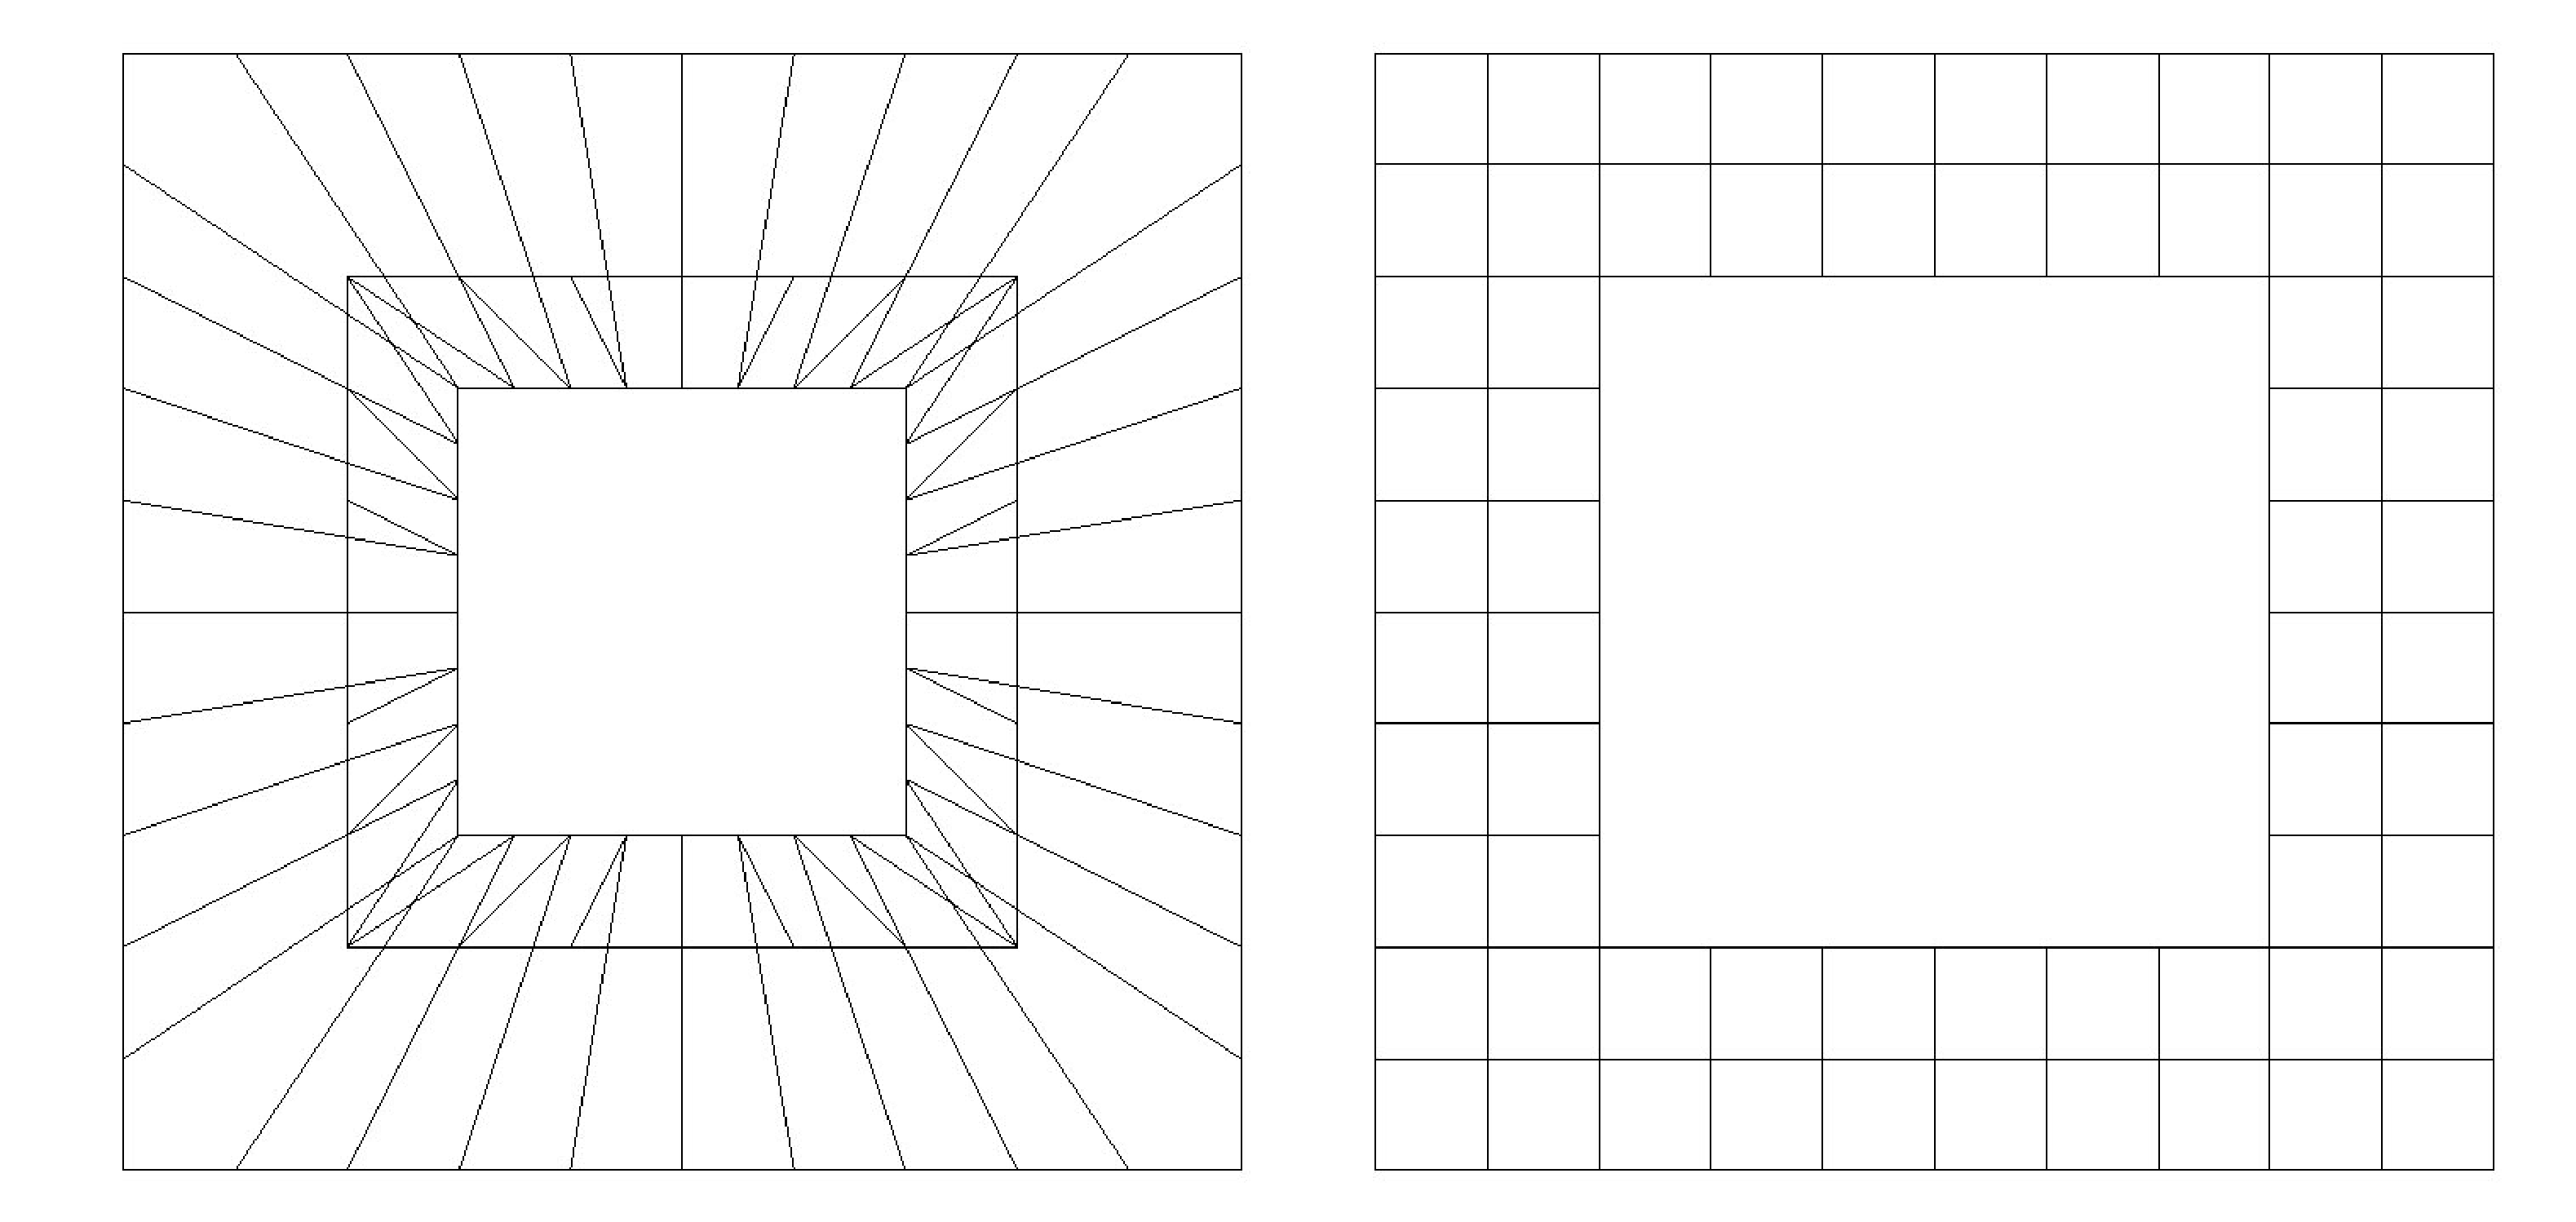
\includegraphics[height=75mm]{inverted-hole-1.eps}
    \caption{LaplaceWrapper, file: inverted-hole-1.vtk mesh. The original mesh is on the left, the mesh smoothed with the \texttt{LaplacianSmoother} is shown on the right.}
    \label{fig:inverted_hole_1}
\end{center}
\end{figure*}

\newpage

\section{Shape-Improvement} \label{sec:ShapeImprover}

\noindent {\it Name}: ShapeImprover \newline
\noindent {\it Purpose}: Make the shape of an element as close as possible to 
that of the ideal/regular element shape. For example, make triangular and 
tetrahedral elements equilateral.  The wrapper will use a non-barrier metric on meshes that contain inverted elements
and will use a barrier metric if the mesh does not contain inverted elements.  The default CPU time limit is 300 seconds.\newline 
\noindent {\it Notes}: There is no guarantee that the wrapper will be able to successfully untangle a mesh that contains inverted elements.\newline
\noindent {\it Limitations/assumptions}:  \newline 
\noindent {\it Input Termination Criterion}: CPU time limit of 300 seconds or maximum absolute vertex movement of 10 percent of the minimum edge length. \newline \newline

\noindent Under the Cover: \newline
\noindent {\it Metric}: TMPQualityMetric(Shape/ShapeBarrier) \newline
\noindent {\it Objective Function}: Algebraic mean of quality metric values \newline
\noindent {\it Mesh/Element Type}: Any supported type. \newline
\noindent {\it Solver}: Conjugate Gradient \newline
\noindent {\it Global/Local}: Global \newline

\noindent Example: \newline

\begin{verbatim}
************** QualityAssessor(free only) Summary **************

  Evaluating quality for 40 elements.
  This mesh had 40 quadrilateral elements.
  There were no inverted elements detected.
  No entities had undefined values for any computed metric.

     Element Quality Statistics

     minimum     average         rms     maximum    std.dev.
   0.0767863    0.232261    0.262717    0.404594    0.122781

     Number of statistics = 40
     Metric = ElementPMeanP(TShapeB1)
     Element Quality not based on sample points.


************** QualityAssessor(free only) Summary **************

  Evaluating quality for 40 elements.
  This mesh had 40 quadrilateral elements.
  There were no inverted elements detected.
  No entities had undefined values for any computed metric.

     Element Quality Statistics

     minimum     average         rms     maximum    std.dev.
    0.124926    0.204118    0.207417    0.328688   0.0368497

     Number of statistics = 40
     Metric = ElementPMeanP(TShapeB1)
     Element Quality not based on sample points.
\end{verbatim}

\begin{figure*}[htbp]
\begin{center}
    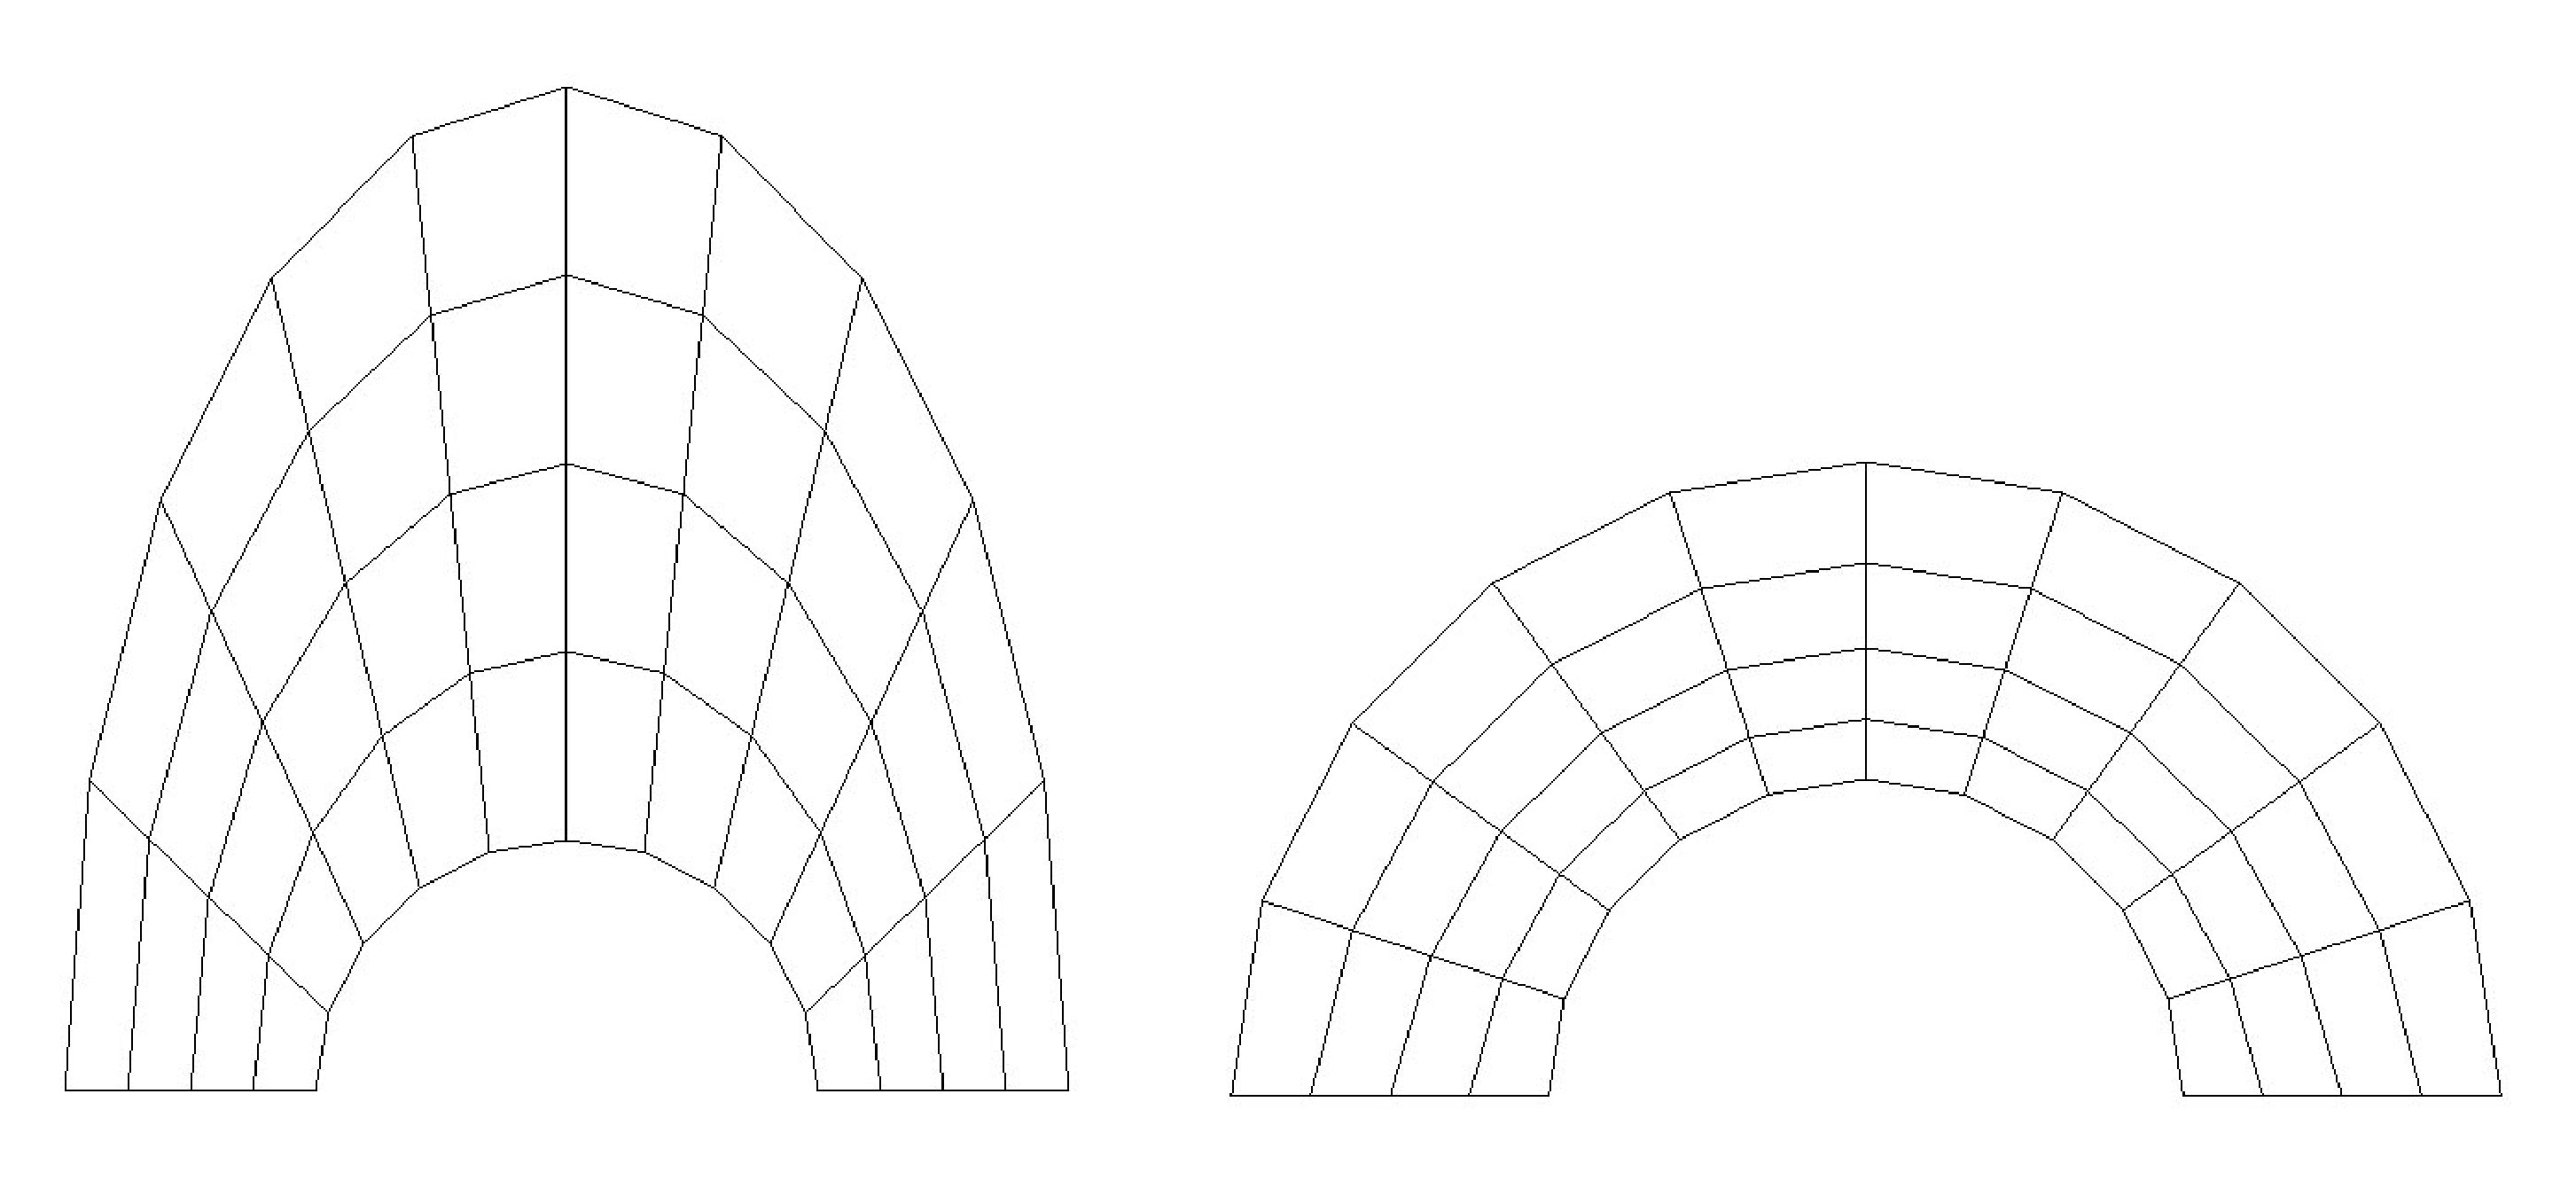
\includegraphics[height=80mm]{horseshoe-10x4.eps}
    \caption{ShapeImproverWrapper, file: tfi\_horse10x4-12.vtk mesh. The original mesh is on the left, the improved mesh is shown on the right.}
    \label{fig:inverted-hole-1}
\end{center}
\end{figure*}

\newpage

\section{Untangler} \label{sec:Untangler}

\noindent {\it Name}: UntangleWrapper \newline
\noindent {\it Purpose}: Untangle elements.  Prioritizes untangling over
element shape or other mesh quality measures.  \newline
\noindent {\it Notes}: A second optimization to improve element quality
after untangling is often necessary.  \newline
\noindent {\it Limitations/assumptions}: There is no guarantee that the optimal mesh computed using this wrapper will, in fact, be untangled.  \newline 
\noindent {\it Input Termination Criterion}: CPU time limit (not used if input 
value is non-positive) or fraction of mean edge length (default is 0.005).  It
also terminates if all elements are untangled, such that it should not modify
an input mesh with no inverted elements. \newline \newline

\noindent Under the Cover: \newline
\noindent {\it Metric}: TUntangleBeta or TUntangleMu(TSizeNB1) or TUntangleMu(TShapeSizeNB1) \newline
\noindent {\it Objective Function}: Algebraic mean of quality metric values \newline
\noindent {\it Mesh/Element Type}: Any supported type. \newline
\noindent {\it Solver}: Steepest Descent \newline
\noindent {\it Global/Local}: Local with culling, optionally Jacobi \newline

\noindent Example: \newline

\begin{verbatim}
************** QualityAssessor(free only) Summary **************

  Evaluating quality for 1024 elements.
  This mesh had 1024 quadrilateral elements.
  THERE ARE 9 INVERTED ELEMENTS.
  (Elements invalid at 9 of 4096 sample locations.)

  No entities had undefined values for any computed metric.

     Element Quality Statistics

     minimum     average         rms     maximum    std.dev.
           0     48.5379     210.965     2915.69     205.305

     Number of statistics = 1024
     Metric = ElementPMeanP(untangle(2D:TShapeSize2DNB1; 3D:TShapeSize3DNB1))
     Element Quality not based on sample points.

************** QualityAssessor(free only) Summary **************

  Evaluating quality for 1024 elements.
  This mesh had 1024 quadrilateral elements.
  There were no inverted elements detected.
  No entities had undefined values for any computed metric.

     Element Quality Statistics

     minimum     average         rms     maximum    std.dev.
           0     1.46636     23.8476     462.591     23.8025

     Number of statistics = 1024
     Metric = ElementPMeanP(untangle(2D:TShapeSize2DNB1; 3D:TShapeSize3DNB1))
     Element Quality not based on sample points.
\end{verbatim}


\begin{figure*}[htbp]
\begin{center}
    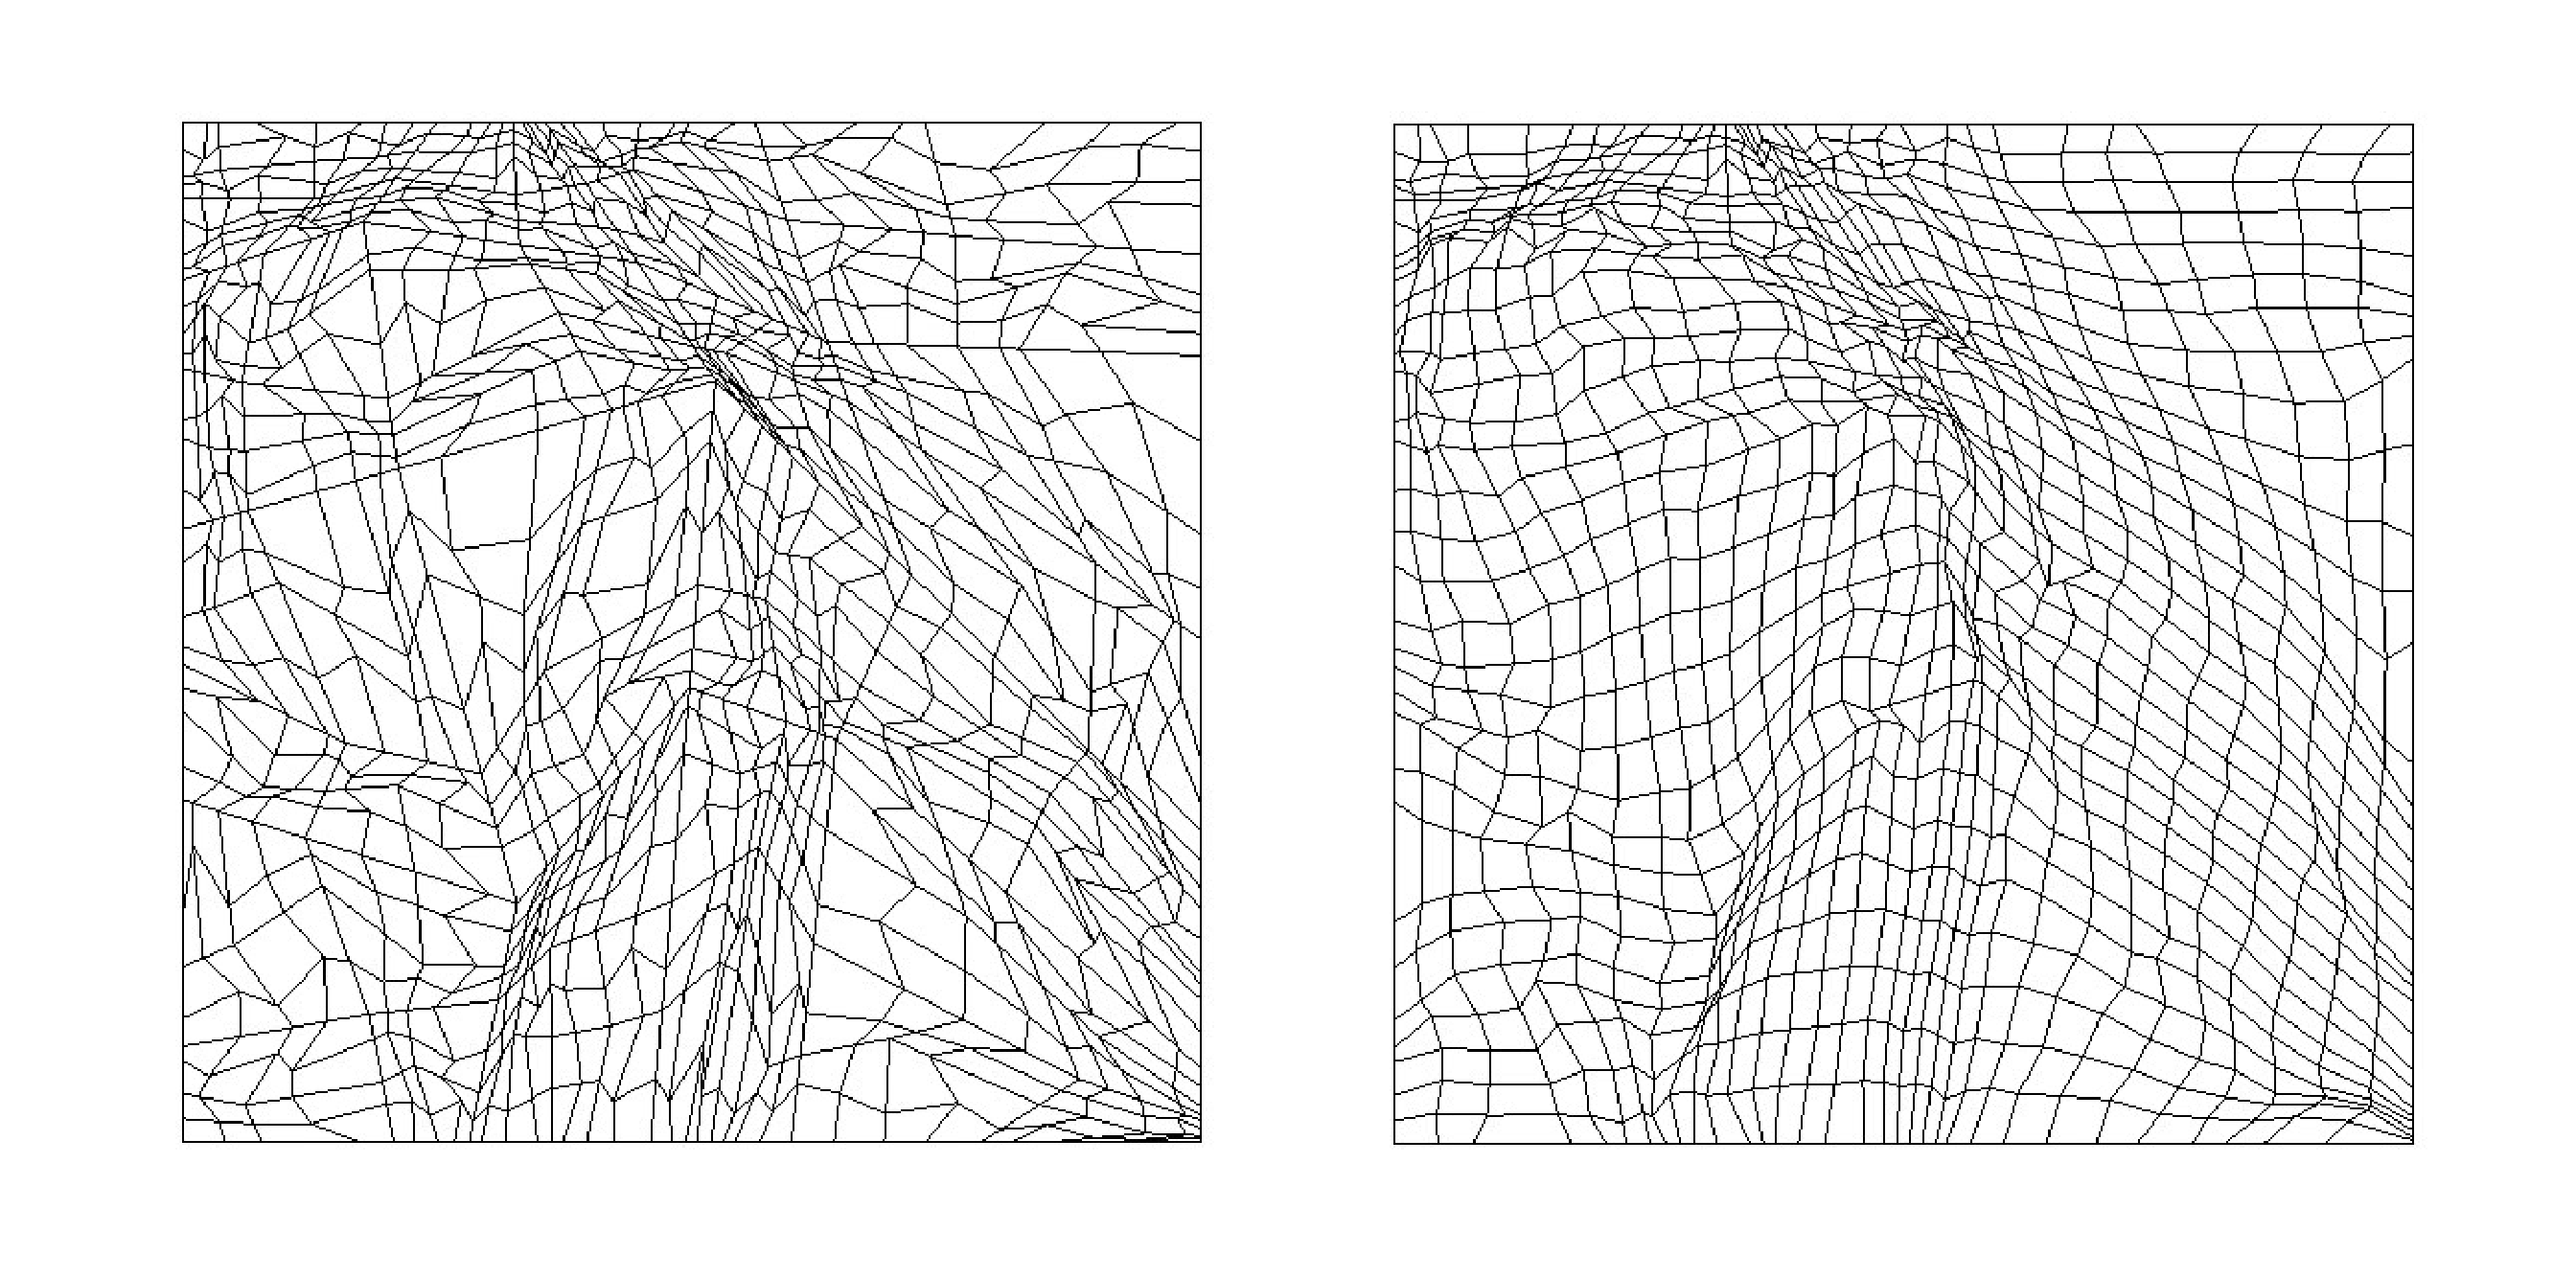
\includegraphics[height=80mm]{shest_grid32.eps}
    \caption{UntangleWrapper, TShapeSizeNB1 option, file: shest\_grid32.vtk mesh. The original mesh is on the left, the untangled mesh is shown on the right.}
    \label{fig:shest_grid32}
\end{center}
\end{figure*}

\newpage

\section{Minimum Edge-Length Improvement} \label{sec:PaverMinEdgeLengthWrapper}

\noindent {\it Name}: PaverMinEdgeLengthWrapper \newline
\noindent {\it Purpose}: Make all the edges in the mesh of equal length while 
moving toward the ideal shape. Intended for explicit PDE codes whose 
time-step limination is governed by the minimum edge-length in the mesh. \newline
\noindent {\it Notes}: Based on Target-matrix paradigm. \newline
\noindent {\it Limitations/assumptions}: Initial mesh must be non-inverted. User does not want to preserve or create anisotropic elements. \newline 
\noindent {\it Input Termination Criterion}: maximum iterations (default=50), maximum absolute vertex movement \newline \newline

\noindent Under the Cover: \newline
\noindent {\it Hardwired Parameters}: None \newline
\noindent {\it Metric}:  Target2DShapeSizeBarrier or Target3DShapeSizeBarrier \newline
\noindent {\it Tradeoff Coefficient}: 1.0 \newline
\noindent {\it Objective Function}: Linear Average over the Sample Points \newline
\noindent {\it Mesh/Element Type}: Any supported type.  \newline
\noindent {\it Solver}: Trust Region \newline
\noindent {\it Global/Local}: Global \newline

\noindent Example: \newline

\begin{verbatim}
************** QualityAssessor(free only) Summary **************

  Evaluating quality for 8 elements.
  This mesh had 8 quadrilateral elements.
  There were no inverted elements detected.
  No entities had undefined values for any computed metric.

     Element Quality Statistics

     minimum     average         rms     maximum    std.dev.
    0.357275    0.983461     1.33806     3.27555    0.907303

     Number of statistics = 8
     Metric = ElementPMeanP(TShapeSizeB1)
     Element Quality not based on sample points.

    -------------------------------------------
     Element Quality Statistics

     minimum     average         rms     maximum    std.dev.
    0.538516     1.11317     1.15398     1.51327    0.304184

     Number of statistics = 12
     Metric = EdgeLength
     Element Quality not based on sample points.



************** QualityAssessor(free only) Summary **************

  Evaluating quality for 8 elements.
  This mesh had 8 quadrilateral elements.
  There were no inverted elements detected.
  No entities had undefined values for any computed metric.

     Element Quality Statistics

     minimum     average         rms     maximum    std.dev.
  0.00135009   0.0017804  0.00179488  0.00221721 0.000227498

     Number of statistics = 8
     Metric = ElementPMeanP(TShapeSizeB1)
     Element Quality not based on sample points.

    -------------------------------------------
     Element Quality Statistics

     minimum     average         rms     maximum    std.dev.
    0.994086      1.0004     1.00041     1.00293  0.00253389

     Number of statistics = 12
     Metric = EdgeLength
     Element Quality not based on sample points.
\end{verbatim}


\begin{figure*}[htbp]
\begin{center}
    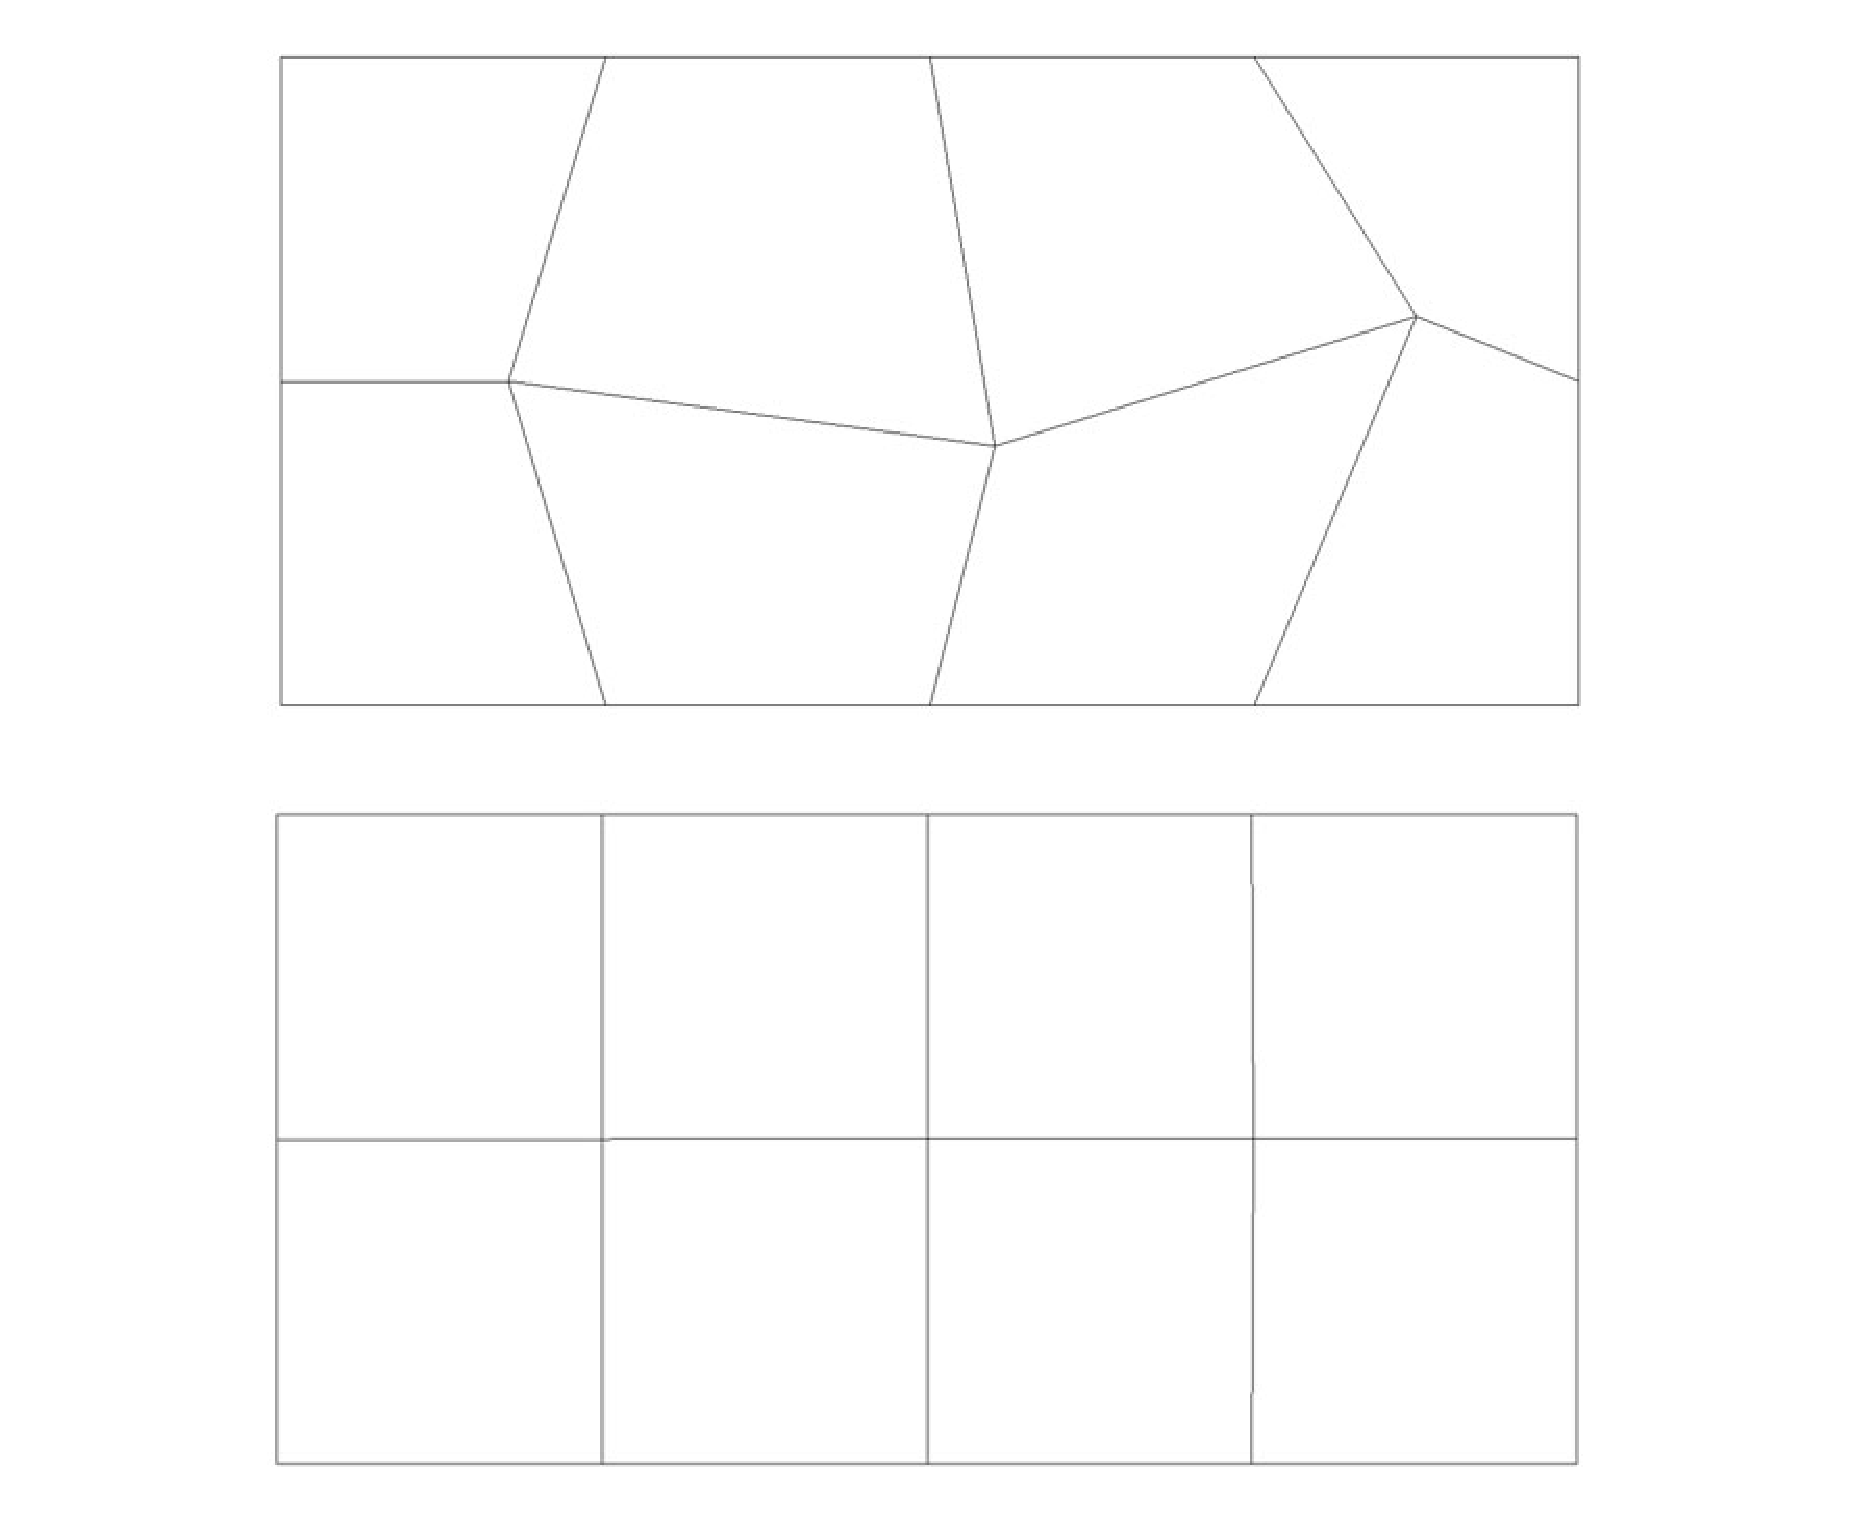
\includegraphics[height=100mm]{min-edge-length.eps}
    \caption{PaverMinEdgeLengthWrapper, file: quads\_4by2\_bad.vtk mesh. The original mesh is on the top, the improved mesh is shown on the bottom.}
    \label{fig:min_edge-length}
\end{center}
\end{figure*}
 
\newpage

\section{Improve the Shapes in a Size-adapted Mesh} \label{sec:SizeAdaptShapeWrapper}

\noindent {\it Name}: SizeAdaptShapeWrapper \newline
\noindent {\it Purpose}: Make the shape of an element as close as possible to that
of the ideal element shape, {\it while preserving, as much as possible, the size of each element in the mesh}. To be used on isotropic initial meshes that are already size-adapted. \newline
\noindent {\it Notes}: Based on Target-matrix Paradigm. \newline
\noindent {\it Limitations/assumptions}: Initial mesh must be non-inverted. 
User wants to preserve sizes of elements in initial mesh and does not want to preserve or 
create anisotropic elements.  \newline 
\noindent {\it Input Termination Criterion}: maximum iterations (default=50), maximum absolute vertex movement \newline \newline

\noindent Under the Cover: \newline
\noindent {\it Hardwired Parameters}: None \newline
\noindent {\it Metric}: Target2DShapeSizeBarrier or Target3DShapeSizeBarrier \newline
\noindent {\it Tradeoff Coefficient}: 1.0 \newline
\noindent {\it Objective Function}: Linear Average over the Sample Points \newline
\noindent {\it Mesh/Element Type}: Any supported type. \newline
\noindent {\it Solver}: Trust Region \newline
\noindent {\it Global/Local}: Global \newline

\noindent Example: \newline

\begin{verbatim}
************** QualityAssessor(free only) Summary **************

  Evaluating quality for 3456 elements.
  This mesh had 3456 quadrilateral elements.
  There were no inverted elements detected.
  No entities had undefined values for any computed metric.

     Element Quality Statistics

     minimum     average         rms     maximum    std.dev.
  0.00447499     0.23505    0.288066    0.710249    0.166533

     Number of statistics = 3456
     Metric = ElementPMeanP(TShapeSizeB1)
     Element Quality not based on sample points.

    -------------------------------------------
     Element Quality Statistics

     minimum     average         rms     maximum    std.dev.
    0.163072    0.574857     0.62062     1.01908      0.2339

     Number of statistics = 13824
     Metric = EdgeLength
     Element Quality not based on sample points.


************** QualityAssessor(free only) Summary **************

  Evaluating quality for 3456 elements.
  This mesh had 3456 quadrilateral elements.
  There were no inverted elements detected.
  No entities had undefined values for any computed metric.

     Element Quality Statistics

     minimum     average         rms     maximum    std.dev.
  0.00558463   0.0591772   0.0767815    0.303106    0.048923

     Number of statistics = 3456
     Metric = ElementPMeanP(TShapeSizeB1)
     Element Quality not based on sample points.

    -------------------------------------------
     Element Quality Statistics

     minimum     average         rms     maximum    std.dev.
    0.161144    0.562074    0.607611     1.11686    0.230789

     Number of statistics = 13824
     Metric = EdgeLength
     Element Quality not based on sample points.
\end{verbatim}


\begin{figure*}[htbp]
\begin{center}
    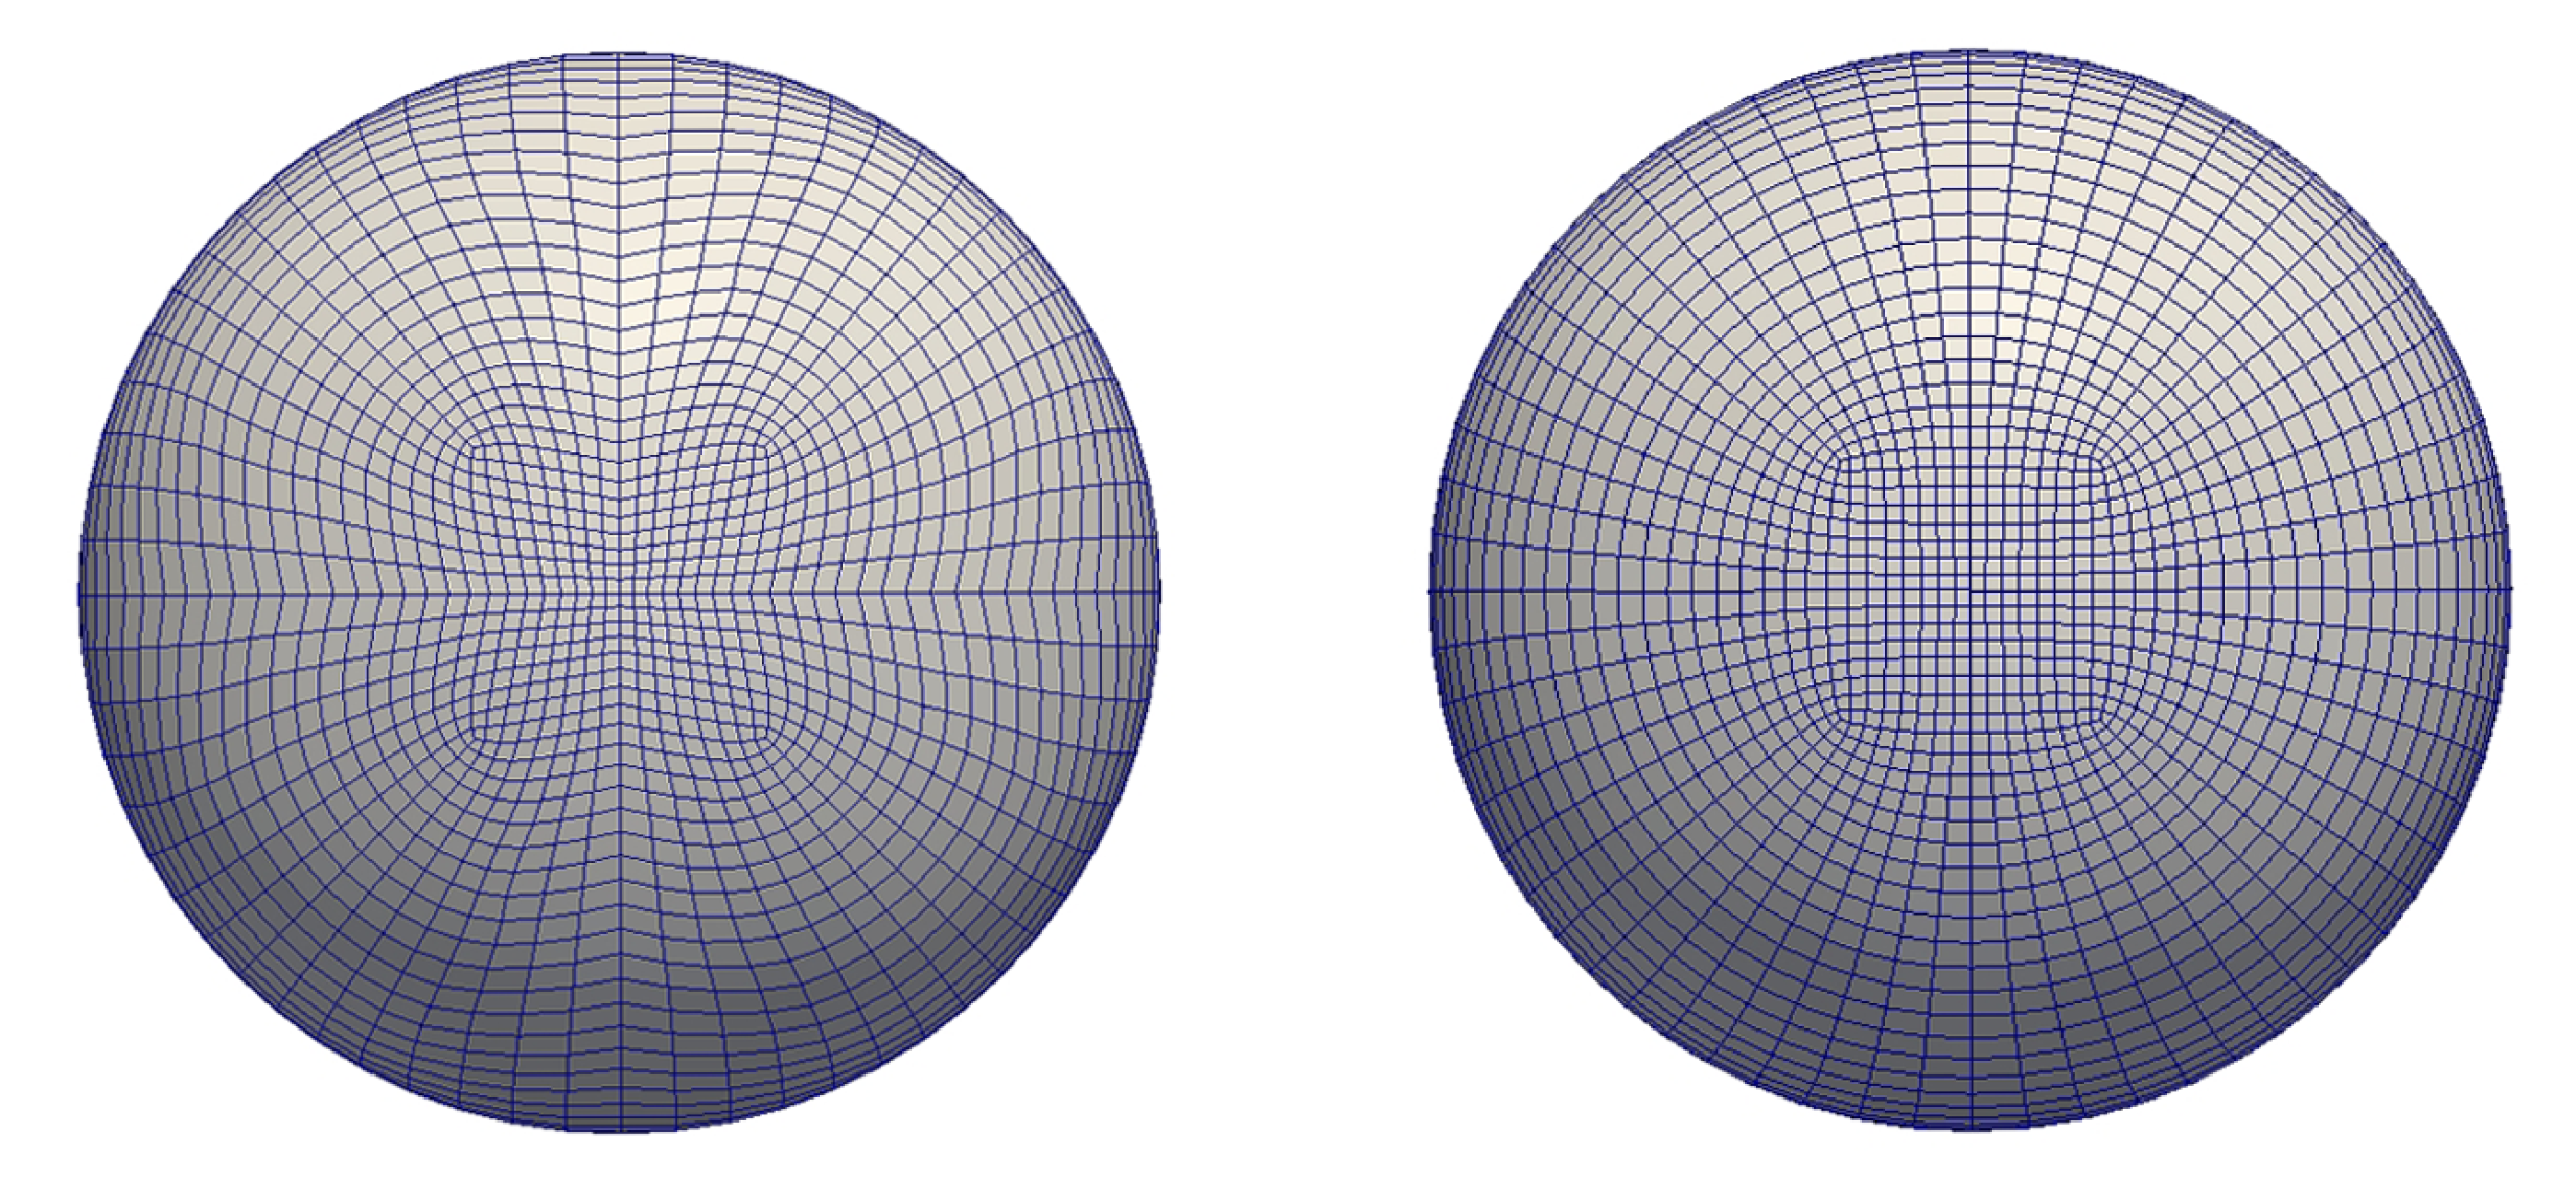
\includegraphics[height=80mm]{bias-sphere-quads.eps}
    \caption{SizeAdaptShapeWrapper, file: bias-sphere-quads.vtk mesh. The original mesh is on the left, the improved mesh is shown on the right.}
    \label{fig:shest_grid32}
\end{center}
\end{figure*}

\newpage

\section{Improve Sliver Tets in a Viscous CFD Mesh} \label{sec:ViscousCFDTetShapeWrapper}

\noindent {\it Name}: ViscousCFDTetShapeWrapper \newline
\noindent {\it Purpose}: Improve the shape of sliver elements in the far-field 
of a CFD mesh while 
preserving an existing layer of sliver elements in the boundary layer. \newline
\noindent Notes: Based on Target-matrix paradigm.  \newline
\noindent {\it Limitations/assumptions}: Tetrahedral meshes only.  \newline 
\noindent {\it Input Termination Criterion}: Iteration Count (default=50) or Maximum Absolution Vertex Movement \newline \newline
 
\noindent Under the Cover: \newline
\noindent {\it Hardwired Parameters}: In tradeoff coefficient model. \newline
\noindent {\it Metric}: Target2DShape+Target2DShapeSizeOrient (or 3D) (or Barrier) \newline
\noindent {\it Tradeoff Coefficient}: Based on element dihedral angle \newline
\noindent {\it Objective Function}: Linear average over Sample Points \newline
\noindent {\it Mesh/Element Type}: Tetrahedra \newline
\noindent {\it Solver}: Trust Region \newline
\noindent {\it Global/Local}: Global \newline


\noindent Additional Information: \newline
\noindent {\it Article}: Introducing the Target-matrix Paradigm for mesh optimization via node-movement", Engineering with Computers, Sept. 2011.\newline

\newpage
\section{Deforming Domain} \label{sec:DeformingDomain}

\noindent {\it Name}: DeformingDomainWrapper \newline
\noindent {\it Purpose}:  Use initial mesh on undeformed geometric domain
to guide optimization of mesh moved to deformed geometric domain.  \newline
\noindent {\it Notes}: Uses a non-barrier metric which means that the
wrapper could potentially invert/tangle elements.  \newline
\noindent {\it Limitations/assumptions}:  Application responsible for explicit handling of mesh on geometric curves and points.  Initial mesh before moving to deformed domain must be available.\newline 
\noindent {\it Input Termination Criterion}: CPU time limit (not used if input 
value is non-positive) or fraction of mean edge length (default is 0.005). \newline \newline

\noindent Under the Cover: \newline
\noindent {\it Metric}: TMPQualityMetric(TShapeNB1 or TShapeSizeNB1 or TShapeSizeOrientNB1) \newline
\noindent {\it Objective Function}: Algebraic mean of quality metric values \newline
\noindent {\it Mesh/Element Type}: Any supported type. \newline
\noindent {\it Solver}: Steepest Descent \newline
\noindent {\it Global/Local}: Local with culling \newline

\noindent Additional Information: \newline
\noindent {\it Article}: "Updating meshes on deforming domains",  Communications in Numerical Methods in Engineering, 24:467-476, 2008..\newline

\noindent Example: \newline

\begin{verbatim}
************** QualityAssessor(free only) Summary **************

  Evaluating quality for 216 elements.
  This mesh had 216 quadrilateral elements.
  THERE ARE 56 INVERTED ELEMENTS.
  (Elements invalid at 220 of 864 sample locations.)

  No entities had undefined values for any computed metric.

     Element Quality Statistics

     minimum     average         rms     maximum    std.dev.
4.57621e-005     7.63416     20.8252     67.0217     19.3754

     Number of statistics = 216
     Metric = ElementPMeanP(TShapeNB1)
     Element Quality not based on sample points.


************** QualityAssessor(free only) Summary **************

  Evaluating quality for 216 elements.
  This mesh had 216 quadrilateral elements.
  There were no inverted elements detected.
  No entities had undefined values for any computed metric.

     Element Quality Statistics

     minimum     average         rms     maximum    std.dev.
 0.000763758   0.0202682   0.0252805   0.0947676   0.0151097

     Number of statistics = 216
     Metric = ElementPMeanP(TShapeNB1)
     Element Quality not based on sample points.
\end{verbatim}


\begin{figure*}[htbp]
\begin{center}
    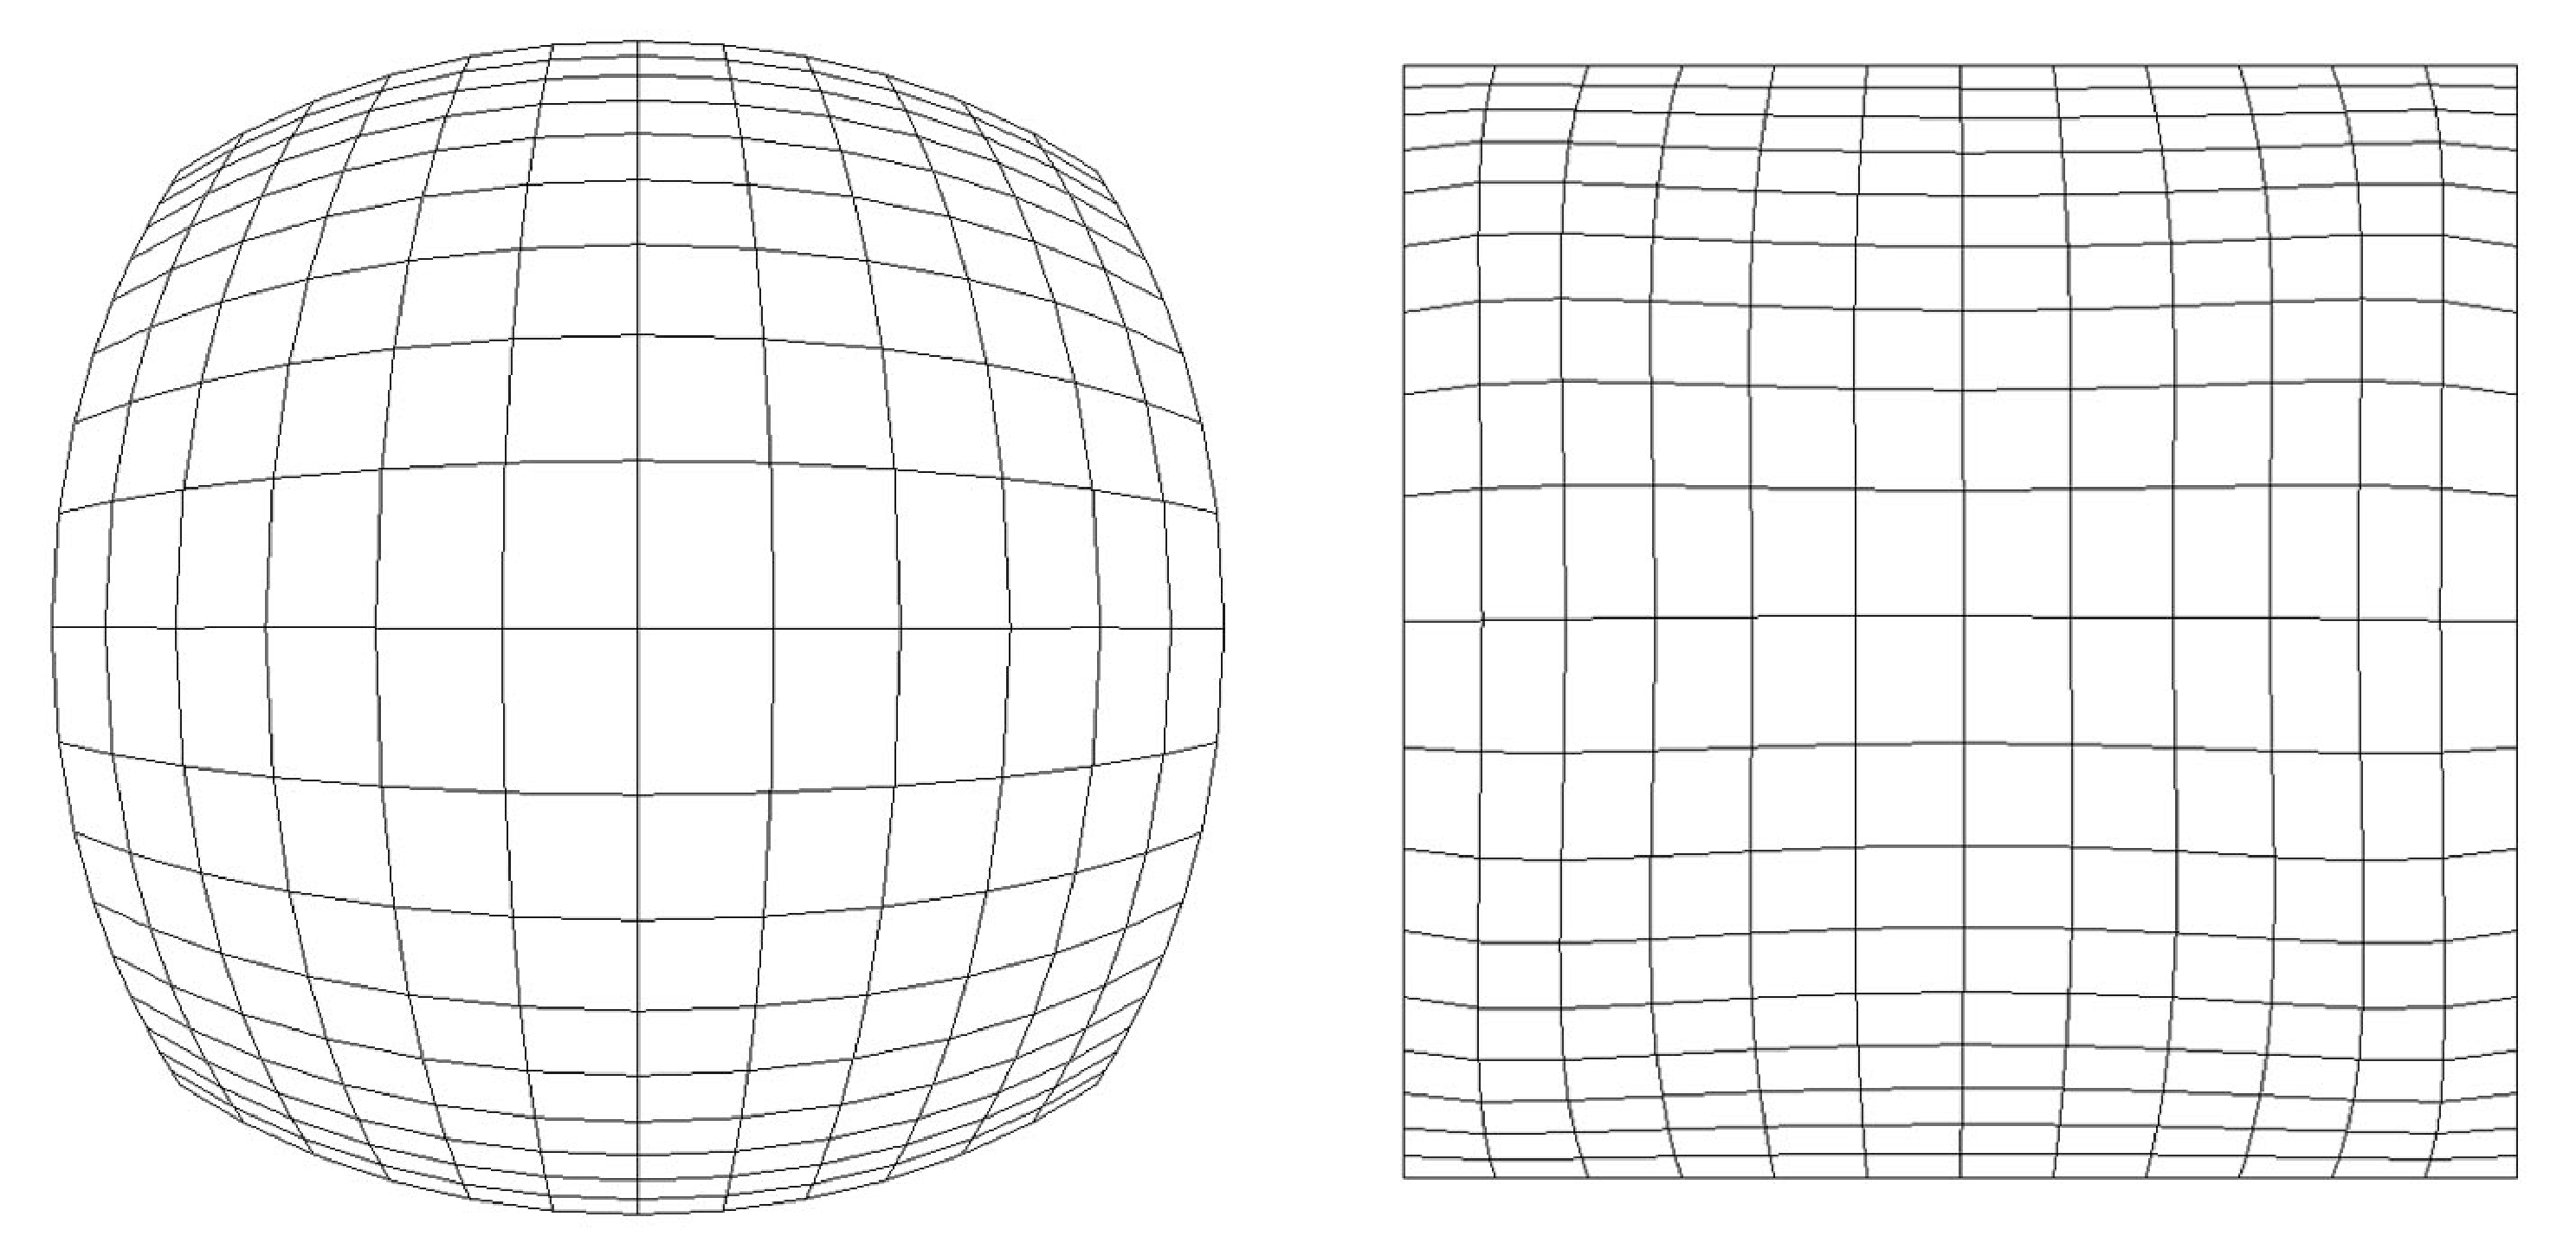
\includegraphics[height=80mm]{sph-10-zsquare.eps}
    \caption{DeformingDomainWrapper, file: sph-10-zsquare.vtk mesh. The original mesh is on the left, the improved mesh is shown on the right.}
    \label{fig:sph-10-zsquare}
\end{center}
\end{figure*}


% Optimization strategies (Nash, global, culling, etc.)
\chapter{Optimization Strategies}

\section{Patches}

\section{Global}

\section{Nash Game}

\section{Block Coordinate Descent}

\section{Culling}

\section{Jacobi}


% Constructing custom solvers - part 1
%\chapter{Constructing Custom Optimization Algorithms}

\section{Algoritm Components}




\section{Quality Metrics}

\section{Objective Functions}

\section{Solvers}

\section{Termination Criteria \label{sec:termination}}


% TMP
%\chapter{Quality Metrics and the Target Matrix Paradigm}

\section{Quality Metric Components}

\section{Target Metrics}

\section{Target Calculators}

\section{Metric Weights}

\section{Custom Target Calculators}



% more TMP stuff
%\chapter{Target Matrix Paradign Advanced Topics}

\section{Inital Mesh and Reference Meshes}

\section{Saving/Restoring Pre-Calculated Targets}

\section{Misc}

\subsection{Caching Targets}



% debugging solvers
\chapter{Analyzing Optimizer Behavior}

This chapter provides a brief overview of some of the tools provided in Mesquite for assisting with the analyze and visualization of the Mesquite optimization process.  The tools discussed in this section can be used to provide additional
output.  External tools such as Paraview, VisIt, or GNU Plot must be used to visualize the data.

\section{Assessing Quality}

  The QualityAssessor class provides a summary of the mesh quality.  An instance of QualityAssessor may be inserted in the InstructionQueue at any point to print a summary of the mesh quality at that time during the optimization.  Instances of the QualityMetric class can be created and passed to the QualityAssessor class to be used to assess the mesh quality.  If no QualityMetrics are specified, the only assessment that will be performed is a simple count of inverted elements.

  A number of constructors are provided by the QualityAssessor class.  Each allows the specification of a different set paramaters to control the quality assement.  The parameters are described below including default values, if any. Note that all paramaters are not used in each constructor.

\label{QA_params}
Parmaters used by QualityAssesor constructors:
\begin{description}
\item[metric:]   QualtiyMetric to register for use in assessing mesh quality.  Will also be used as the "stopping assessment".

\item[historgram\_intervals:]   If non-zero, a histogram of quality metric values composed of the specified number of intervals will be generated.  Default is zero.
\item[power\_mean:] If non-zero, in addition to the normal summary statistics for the quality metric, an additional general power mean with the specified power will be calculated.  Default is zero.

\item[free\_elements\_only:] If true, only quality values that depend on at least one free vertex will be used. Default is true.

\item[inverted\_element\_tag\_name:] If a non-null value is specified, an integer tag with the specified name will be used to store a value of 0 for normal elements and 1 for inverted elements.  Default is null value.

\item[metric\_value\_tag\_name:] If a non-null value is specified, a tag with the specified name will be populated with quality values for individual elements or vertices if metric is an element-based or vertex-based metric.  If metric is not element-based or vertex-based, this argument has no effect.  Default is null value.

\item[print\_summary\_to\_std\_out:] If true, summary of mesh quality will be written to std::out.  If false, quality assessment will be available via the get\_results and get\_all\_results methods, but will not be printed.  Default is true.

\item[output\_stream IO:] stream to which to write a summary of the mesh quality.

\item[name:] Name to include in output.  Useful if several QualityAssessors are in use at the same time.
\end{description}

  After the QualityAssessor instance is created, any of a number of methods 
can be used to set individual characteristics of the QualityAssessor object.

  Once setup for the QualityAssessor object  is complete, the actual assement is preformed by calling "loop\_over\_mesh".  After it terminates, results can be obtained using various methods supplied by the QualityAssessor class.


A simple example using the QualityAssessor class:
\begin{lstlisting}[frame=single]
  MsqError err;
  MeshImpl meshToAssess;
  PlanarDomain myDomain;
  Settings mySettings;

  meshToAssess.clear();

    // read in mesh
  const char* filename = "meshToAssess.vtk";
  meshToAssess.read_vtk( filename, err);

    // create metric instance
  ConditionNumberQualityMetric metric;

    // create QualityAssessor instance accepting default values
  QualityAssessor qa( &metric );

    // change some of the default paramaters
  qa.measure_free_samples_only( false );
  qa.disable_printing_results();

    // run the QualityAssessor
  qa.loop_over_mesh( &meshToAssess, &myDomain, &mySettings, err  );

    // get results
  const QualityAssessor::Assessor* results = qa.get_results( &metric );
  int invalid_element_count = results->get_invalid_element_count();
  if ( invalid_element_count != 0 )
    std::cout << "Warning: " << invalid_element_count 
                        << " invalid elements found." << std::endl;
\end{lstlisting}

\section{Debug Output}

Mesquite contains a mechanism to send status and debug messages to an output stream (e.g. {\texttt stdout} or {\texttt std::cout}).  Debug messages are grouped into logical categories identified by an integer number.  For example debug flag 1 refers to warnings.  Debug flag 2 is used for status information about the outer optimization loop, and debug flag 3 is used for status of the inner optimization loop. 

Debug flags can be controlled through a variety of means.  The {\texttt --enable-debug-output} configure option can be specified with a comma-separated list of integer values to specify which debug groups should be enabled by default.  An application may call the {\texttt MsqDebug::enable(unsigned)} and {\texttt MsqDebug::disable(unsigned)} functions to enable or disable debug message groups.  Debug message groups may also be controlled with the environmental variables {\texttt MESQUITE\_DEBUG} and {\texttt MESQUITE\_NO\_DEBUG}.  Each should have a comma-separated list of integer values as its argument.  The variables enable and disable, respectively, the corresponding debug message groups.

\section{Plotting Convergence Behavior \label{sec:optplot}}

The Mesquite {\texttt TerminationCriterion} class can produce a simple table of tab-separated values for the different Mesquite termination criterion.  This file can be used to plot the behavior of the optimization loop using GNU Plot, a spread sheet application, or any other suitable tool.  The code listing below illustrates how this feature is activated.

\begin{lstlisting}[frame=single]
// Create global optimizer instance
SteepestDescent improver( &objective_function );
improver.use_global_patch();

// Set only inner termination criterion for 
// global optimization
TerminationCriterion inner;
inner.add_absolute_vertex_movement( 1e-3 );
\<inner.write_iterations( "plot.gpt" );\>
improver.set_inner_termination_criterion( &inner );

// Run optimization
InstructionQueue queue;
queue.set_master_quality_improver( &improver, err );
queue.run_instructions( &mesh, err );
\end{lstlisting}

For usable results the feature must be activated on the appropriate {\texttt TerminationCriterion} instance.  For a global optimization it should be enabled for the {\em inner} termination criterion.  For other optimization strategies (see Chapter \ref{ch:optstrat}) it should be enabled for the {\em outer} termination criterion.  

The following is a sample output file:

\begin{lstlisting}[basicstyle=\small,language=make]
#Iter	CPU	ObjFunc	GradL2	GradInf	Movement	Inverted
0	0	1.47419	0	0	0	0
1	0	1.147	0	0	0.657155	0
2	0	1.04779	0	0	0.402173	0
3	0	1.00572	0	0	0.357444	0
4	0	1.00006	0	0	0.150652	0
5	0	1	0	0	0.0153396	0
6	0	1	0	0	0.00015034	0
7	0	1	0	0	6.40008e-09	0
\end{lstlisting}

Notice that several of the columns contain only zeros.  The column containing the iteration number will always contain valid values.  Other values will only be included if they are calculated during the optimization loop.  The objective function value will be included for any global optimization that uses an explicit objective function (currently any optimizer other than {\texttt LaplacianSmoother}).  In the example source code above we are using the steepest descent solver with a global patch so the objective function value is also included.  The other values will only be present if they are calculated for the purpose of checking termination criteria.  In the example source code we specify a termination criterion based on vertex movement, so the column labeled ``movement'' contains the maximum distance any vertex was moved for the corresponding iteration.  

Figures \ref{fig:iterplot} shows the result of using the above data file with the following GNU Plot commands:
\begin{verbatim}
set xlabel 'iterations'
set ylabel 'objective function value'
set y2label 'maximum vertex movement'
set y2tics 0.1
plot 'plot.gpt' using 1:3 with linespoints \
     title 'objective function', \
     'plot.gpt' using 1:6 axes x1y2 with \
     linespoints title 'vertex movement'
\end{verbatim}

\begin{figure}[htb!]
\begin{center}
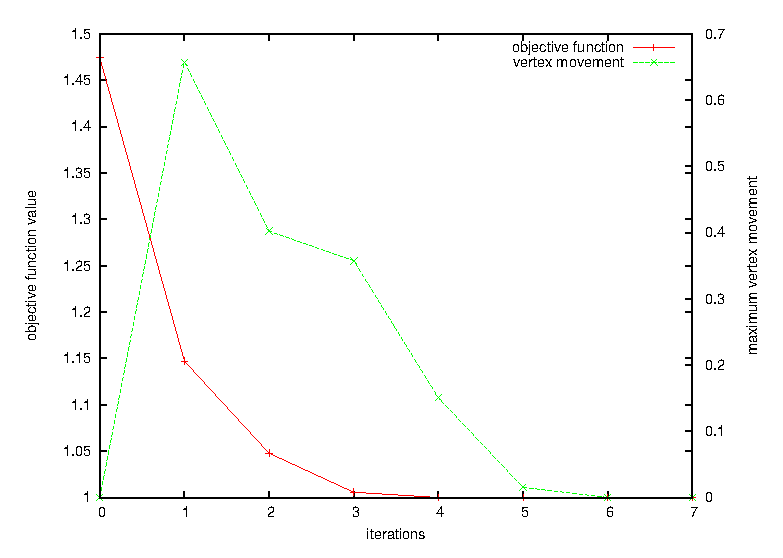
\includegraphics[width=5in]{iterplot}
\caption{\em Convergence Plot \label{fig:iterplot}}
\end{center}
\end{figure}

\section{Viewing Meshes}

VTK files read and written by the {\texttt MeshImpl} class are viewable in a plethora of visualization tools that use the VTK visualization library.  

The {\texttt Mesquite::MeshWriter} namespace contains functions to export mesh in a variety of formats for visualization including:
\begin{itemize}
\item GNU Plot
\item Visualization TookKit (VTK)
\item Encapsulated PostScript (EPS)
\item Scalable Vector Graphics (SVG)
\item StereoLithography (STL)
\end{itemize}
The GNU plot format writes line data that can be used to plot a wireframe of the mesh (the mesh edges).  Both 2D and 3D meshes can be exported in this format.  A mesh can be plotted as a 2D projection with the GNU plot command:
\begin{verbatim}
plot 'filename' with linespoints
\end{verbatim}
or as a rotatable 3D plot with the command:
\begin{verbatim}
splot 'filename' with linespoints
\end{verbatim}
Figure \ref{fig:meshgpt} is the result of plotting the mesh contained in {\texttt testSuite/higher\_order/homogeneousPart.vtk} with GNU plot.

\begin{figure}[htb!]
\begin{center}
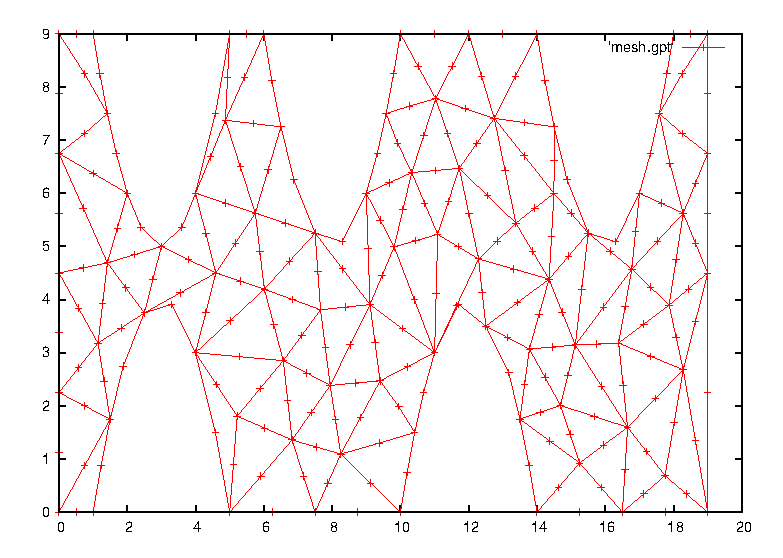
\includegraphics[width=4in]{mesh_gpt}
\caption{\em GNU Plot of 2D Quadratic Triangles \label{fig:meshgpt}}
\end{center}
\end{figure}

As mentioned in the previous section, the VTK file format can be used with a variety of visualization tools.  Figure \ref{fig:meshvtk} shows a simple plot of the same mesh in the Paraview visualization tool.

\begin{figure}[htb!]
\begin{center}
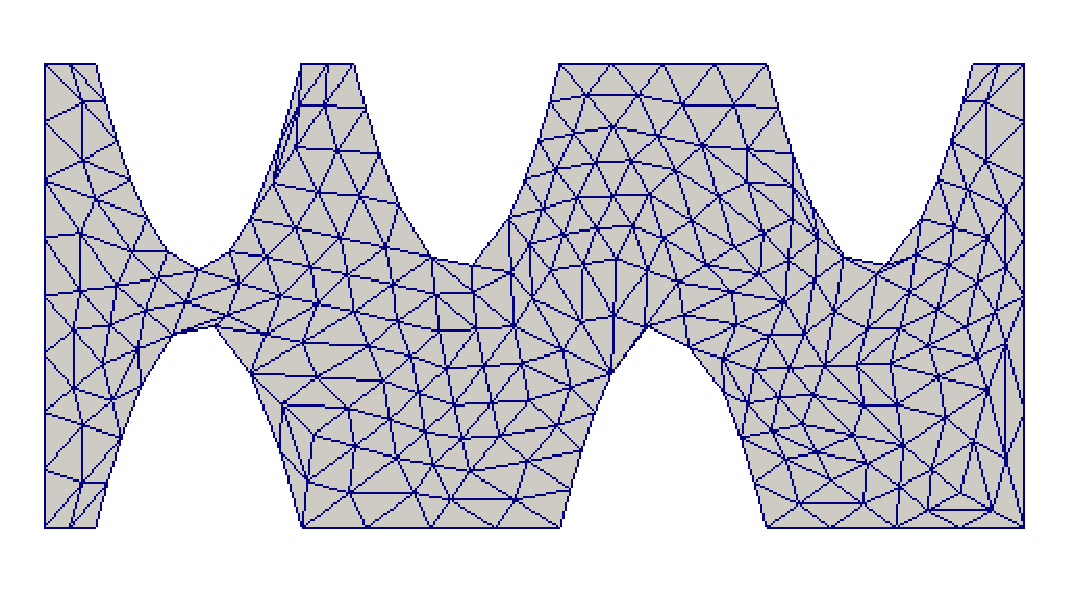
\includegraphics[width=4in]{mesh_vtk}
\caption{\em Paraview plot of 2D Quadratic Triangles \label{fig:meshvtk}}
\end{center}
\end{figure}

Figure \ref{fig:mesh} shows the output of the encapsulated PostScript writer for the mesh.  The EPS writer can write only 2D projections of the mesh.  The caller must specify a projection when calling {\texttt MeshWriter::write\_eps}.  The {\texttt testSuite/higher\_order/homogeneousPart.vtk} file contains quadratic triangle elements.  Compare the mesh edges on the mesh boundary in this plot with the output in Figures \ref{fig:meshgpt} and \ref{fig:meshvtk}.  The EPS writer in Mesquite exports the quadratic edges as curves corresponding to the classic quadratic edge shape function:
\begin{displaymath}
E(u) = \frac{1}{2}u(u-1)V_1 + (1-u^2)V_2 + \frac{1}{2}u(u+1)V_3
\end{displaymath}

\begin{figure}[htb!]
\begin{center}
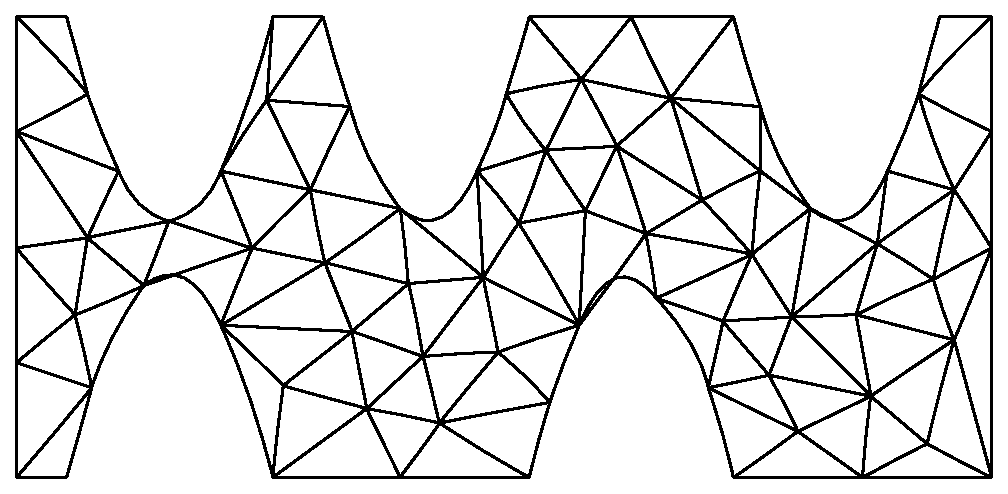
\includegraphics[width=4in]{mesh}
\caption{\em Encapsulated PostScript of 2D Quadratic Triangles \label{fig:mesh}}
\end{center}
\end{figure}

The STL file format can be used to write only linear triangles.  Higher-order triangular elements will be written as linear triangles.  An error will be returned if the mesh contains other element types.

\section{Exporting Mesh Quality}

The {\texttt QualityAssessor} class has the ability to store mesh quality values and other characteristics as tag data on mesh elements.  This data can be accessed directly by applications or written to a VTK file using the {\texttt MeshImpl} class or the applications native mesh writer (if it is capable of writing tag data.)  The example code below was used to create the VTK file from which the Paraview plot in Figure \ref{fig:meshqual} was generated.

\begin{figure}[htb!]
\begin{center}
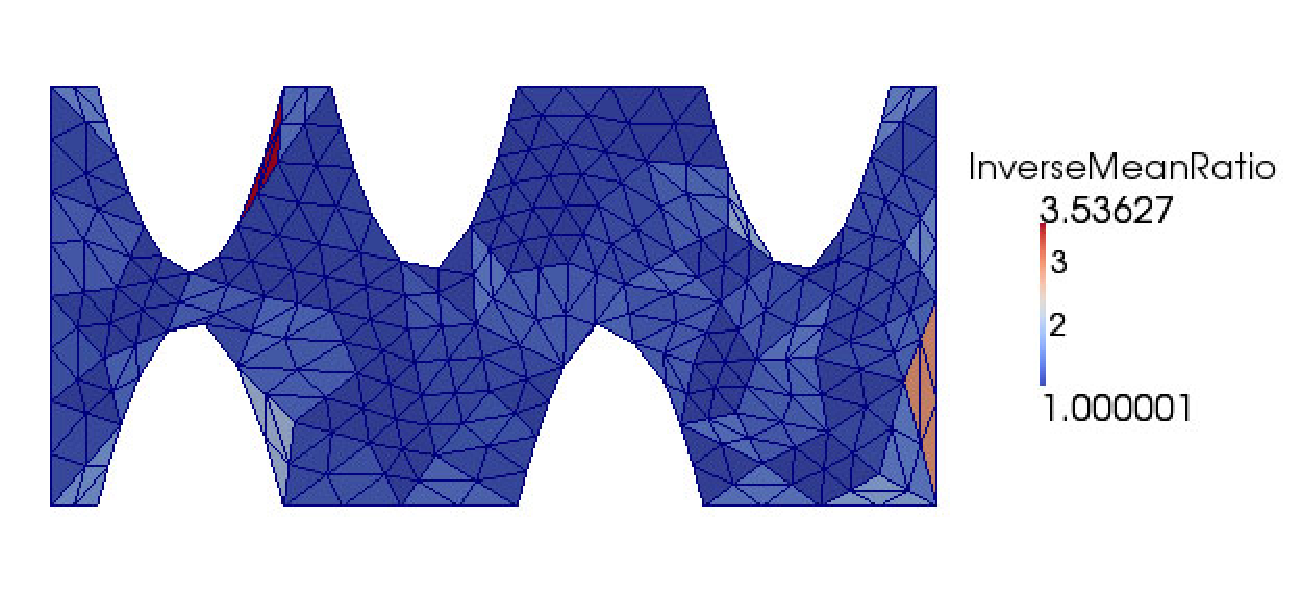
\includegraphics[width=5in]{meshqual}
\caption{\em Paraview Plot Coloring Elements by Quality Metric Value \label{fig:meshqual}}
\end{center}
\end{figure}

\newpage
\begin{samepage}
\begin{lstlisting}[frame=single]
MsqError err;
MeshImpl mesh;
mesh.read_vtk( "homogeneousPart.vtk", err );

IdealWeightInverseMeanRatio metric;
QualityAssessor qa;
qa.add_quality_assessment(&metric,0,0,0,\<"InverseMeanRatio"\>);

PlanarDomain plane(PlanarDomain::XY);
InstructionQueue queue;
queue.add_quality_assessor( &qa, err );
queue.run_instructions( &mesh, &plane, err );

mesh.write_vtk( "meshqual.vtk", err );
\end{lstlisting}
\end{samepage}

\begin{figure}[htb!]
\begin{center}
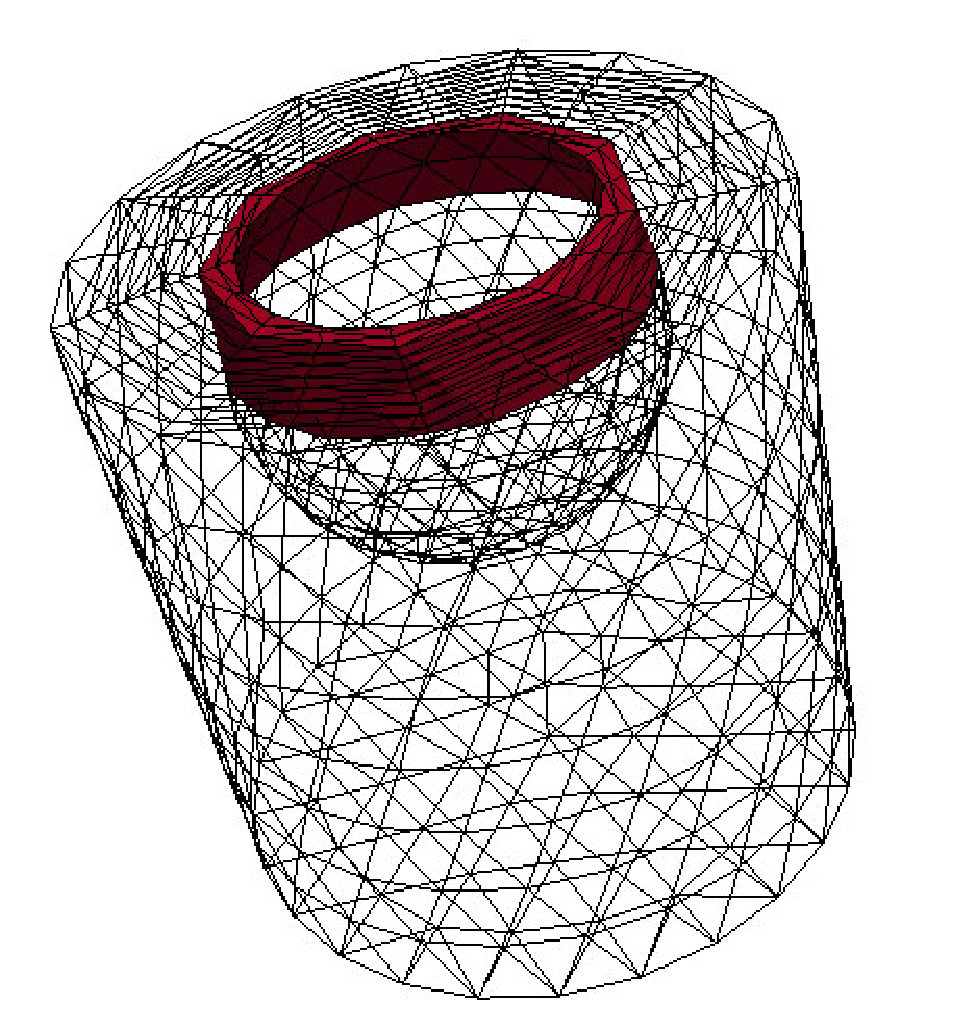
\includegraphics[width=3in]{meshqual3d}
\caption{\em Paraview Plot Showing Inverted Elements \label{fig:meshqual3d}}
\end{center}
\end{figure}

Figure \ref{fig:meshqual3d} is a Paraview plot showing the inverted elements in a quadratic tetrahedral mesh.  The mesh is plotted twice: once as a simple wireframe of the mesh boundary and a second time as solid mesh with a threshold filter on the inverted flag exported by Mesquite.  The listing below shows how the {\texttt QualityAssessor} class can be instructed to flag inverted elements:

\newpage
\begin{lstlisting}[frame=single]
MsqError err;
MeshImpl mesh;
mesh.read_vtk( "sphereCylinder_1194_inv.vtk", err );

QualityAssessor qa;
\<qa.tag_inverted_elements("Inverted");\>

InstructionQueue queue;
queue.add_quality_assessor( &qa, err );
queue.run_instructions( &mesh, &plane, err );

mesh.write_vtk( "meshqual.vtk", err );
\end{lstlisting}


\section{Mesh Optimization Visualization}

The Mesquite {\texttt TerminationCriterion} class can write the complete mesh after each iteration as either VTK or GNU Plot data suitable for viewing as an animation.  Similar to requesting plot data as described in Section {\ref sec:optplot}, it is important to request this feature from the appropriate termination criterion instance.  If doing a global optimization, the feature should be activated for the {\em inner} termination criterion.  Otherwise the feature should almost always be activated for the {\em outer} termination criterion.  

The command to request an animation of the mesh optimization in the VTK format is:
\begin{lstlisting}
tc.write_mesh_steps( "anim", TerminationCriterion::VTK );
\end{lstlisting}
This will produce a sequence of files named ``anim.1.vtk'', ``anim.2.vtk'', etc.  The files can be opened in visualization tools such as Paraview as a single set and played back as an animation.  If the optimization calculates the gradient of the objective function, that data will also be included in the file as vector data on each mesh vertex.  The components of the vector on each vertex are the partial derivatives of the objective function with respect to each coordinate value of the vertex.  A Paraview ``glyph'' filter can be used to display these vector values during the animation.


The command to request an animation of the mesh optimization in a format suitable for animating in GNU plot is:
\begin{lstlisting}
tc.write_mesh_steps( "anim", TerminationCriterion::GNUPLOT );
\end{lstlisting}
This will produce a sequence of files named ``anim.1'', ``anim.2'', etc.  It will also export a file named ``anim'' that contains the necessary GNU Plot commands to display the animation.





% Parallel Mesquite
\chapter{Using Mesquite in Parallel}
\label{sec:parallel}

\section{Introduction}

Large meshes are often partitioned across many parallel processors either because they are too large to fit into the memory of a single machine or in order to speed up the computation. Even if it would be possible to assemble all partitions on a single processor, smooth the mesh, and repartition the result, such an approach would be very I/O inefficient. Moreover, for larger meshes such an approach would quickly run out of memory and fail. Therefore Mesquite supports smoothing meshes in parallel.

Mesquite currently does only synchronous Nash-game or local optimizations in parallel \cite{Fr95}.  It does not yet provide parallel solvers and therefore cannot do either block coordinate descent or truly global optimizations in parallel (minimization of an explicit, global objective function.)

For algorithms such as Laplacian smoothing that are local optimizations, optimization in parallel is essentially the same as in serial.  For other optimizations that do a global minimization of an explicitly defined objective function in serial (for example \texttt{ShapeImprover}), the parallel optimization will be a Nash-game type optimization where the interior vertices (those not on the partition boundaries) will be optimized as a group.  Each vertex on the partition boundary will then be optimized individually.  While a global optimization in serial will typically have only one outer iteration, it is generally desirable to do multiple outer iterations in parallel so the Nash-game type optimization can reach convergence.  Mesquite wrappers (see Chapter \ref{sec:wrappers}) that implement global optimizations in serial default to 10 outer iterations in parallel.


\section{Distributed Mesh}

The input mesh for use in parallel quality improvement must be partitioned based on vertices.  That is, each vertex in the mesh must be assigned a single processor as its owner.  For optimal performance, vertices should be evenly distributed amongst available processors and the vertices assigned to the same processor should compose a contiguously connected patch of mesh.

Each processor must also have access to all elements for which the position of its vertices influence the quality.  For almost all algorithms in Mesquite, this is the set of all elements that contain one of the vertices.  Further, each processor must also be able to access any additional vertices owned by other processors that are necessary to define those elements.  The instances of such vertices on processors that do not own them are typically referred to as ``ghosted'' vertices.  Elements for which copies exist on multiple processors may sometimes also be referred to as ``ghosted'' or ``ghost'' elements.

\begin{figure*}[htbp]
\begin{center}
    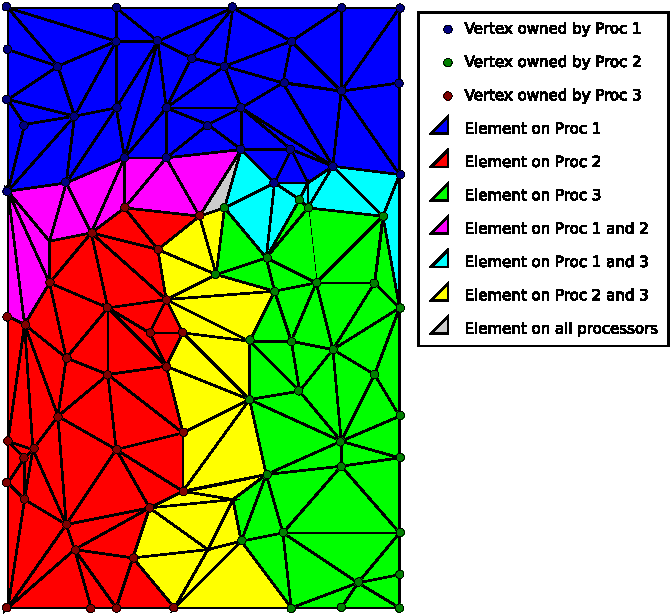
\includegraphics{figures/parallel_mesh}
    \caption{Sharing or ghosting of elements and vertices in a partitioned mesh.}
    \label{fig:parallel_mesh}
\end{center}
\end{figure*}

Figure \ref{fig:parallel_mesh} shows a mesh partitioned amongst three processors.  The vertices owned by the three different processors are shown in three different colors: blue, red, and green.  Elements are colored according to the processors for which copies of that element must be available.  A copy of an element must be available on each processor owning at least one of the vertices of the element.  Elements colored blue, red, or green need be visible only on the processor owning vertices of the corresponding color. The single grey element must have copies defined on all three processors because each of its vertices is owned by a different processor.  The remaining elements must be defined on at least two processors.

For a copy of an element to be available on a processor, all of its vertices must also be available on that processor.  So for all elements for which copies exist on more than one processor, the vertices contained in those elements must also exist as ghost vertices on at least one processor.  That is, copies of such vertices must exist on processors other than those that are responsible for optimizing the location of that vertex.  For example, copies of the yellow elements in Figure \ref{fig:parallel_mesh} exist on both the blue and the green processors.  All blue vertices in at least one yellow element must exist as ghost vertices on the green processor and all green vertices in at least one yellow element exist as ghost copies on the blue processor.  A copy of the grey element must exist on every processor.  Therefore each vertex in that element exist as ghost copies on both of the other two processors that do not own it.


\section{Input Data}

Assuming the mesh exists in partitioned form the user has to provide Mesquite with three things:
\begin{itemize}
\item a processor ID of type \texttt{int} for every vertex that determines which processor owns a vertex and is in charge for smoothing this vertex,
\item a global ID of type \texttt{size\_t} for every vertex that (at least in combination with the processor ID) is globally unique,
\item all necessary ghost elements and ghost nodes along the partition boundary must be provided.
\end{itemize}

The following copies of elements and vertices must exist: Elements must exist on all processors that own one or more of the vertices they reference. Vertices must exist on all processors that have some element referencing them.

The \texttt{Mesquite::ParallelMesh} class (\texttt{ParallelMeshInterface.hpp}) inherits \texttt{Mesquite::Mesh} and defines the interface Mesquite uses to interact with parallel mesh data. It contains the following additional pure virtual (or abstract) functions:
\begin{itemize}
\item get processor ids for given vertices,
\item get global ids for given vertices,
\item set and get a pointer to a \texttt{Mesquite::ParallelHelper} object.
\end{itemize}

To allow Mesquite direct access to the way you store the parallel mesh data you must inherit \texttt{Mesquite::ParallelMesh} and also implement your own get processor ID and get global ID functionality. The \texttt{Mesquite::ParallelHelper} class takes care of all the underlying communication using MPI. You will always use the \texttt{Mesquite::ParallelHelperImpl} implementation that we provide.

Alternatively you can turn any existing mesh of type \texttt{Mesquite::Mesh} into a parallel mesh of type\vspace{-5pt} \begin{center}
\texttt{Mesquite::ParallelMesh} by using the \texttt{Mesquite::ParallelMeshImpl}
\end{center} \vspace{-5 pt}implementation we provide. On creation it needs a pointer to an object of type \texttt{Mesquite::Mesh} and the names of two tags. It is expected that every vertex is properly tagged with the processor ID tag being of type INT and the global ID tag being of type HANDLE.


\subsection{ParallelMesh Implementation Requirements}
%%(this text needs to be added where GLOBAL_ID etc is discussed)

In addition to global and processor ID's, a tag named \texttt{LOCAL\_ID}, with type \texttt{INT}, must be provided in
your ParallelMesh implementation.  In summary, here are the tags and
their types required by Parallel Mesquite:

\begin{tabular}{ | l | l | l | }
  \hline
  Concept name & Typical/required code string &  Mesquite type \\
\hline
 vertex processor owner id & \texttt{PROCESSOR\_ID} (typical, implementation-dependent) & INT \\
 vertex global unique id & \texttt{GLOBAL\_ID} (typical,  implementation-dependent) & HANDLE \\
 vertex local id (internal use) & \texttt{LOCAL\_ID} (required) & INT \\
  \hline
\end{tabular}

If you obtained Mesquite from the Trilinos site, you can see a sample
imlementation of ParallelMesh in the stk\_percept package, at

\texttt{Trilinos/packages/stk/stk\_percept/stk\_percept/mesh/mod/mesquite-interface/PerceptMesquiteMesh.*pp.}

\section{ITAPS iMeshP Interface}

The MsqIMeshP class is an alternate implementation of the \texttt{ParallelMesh} interface that can be used to provide Mesquite with callbacks to access mesh and related parallel properties.  The ITAPS Working Group has defined a standard API for exchange of parallel mesh data between applications. The \texttt{Mesquite::MsqIMeshP} class declared in \texttt{MsqIMeshP.hpp} is an ``adaptor'':  it presents the iMeshP interface as the \texttt{Mesquite::ParallelMesh} interface.

This class will use the iMeshP API to query processor identifiers and global identifiers for mesh vertices.  However, the MPI-based communication routines implemented in \texttt{ParallelHelperImpl} are used rather to communicate updated vertex locations between processors, rather than the mechanism provided by the iMeshP implementation.

\section{Examples}

This section contains two different examples of simple stand-alone applications that demonstrate the use of the \texttt{LaplaceWrapper} smoother in parallel.  Both examples, in being stand-alone programs, load the mesh from one or more files.  When integrating Mesquite into an existing application where it is desired that Mesquite access application mesh data in memory, the initial setup will be different.  It will typically involve either providing some application-specific implementation of the \texttt{Mesh} and possibly \texttt{ParallelMesh} interfaces or instances of an appliction-specific \texttt{iMeshP} and \texttt{iMesh} implementation.

\subsection{Example: Parallel Laplacian Smooth}
\label{sec:parallel-example-1}

This example uses the \texttt{LaplaceWrapper} wrapper in parallel using the built-in \texttt{Mesh}, \texttt{ParallelMesh}, and \texttt{ParallelHelperImpl} implementations.  For this example to work, the mesh must be partitioned such that the mesh for each processor is saved in a separate file named \texttt{part-\%d.vtk}, with the \texttt{\%d} replaced with the processor rank.  Each VTK file must contain vertex attributes named \texttt{GID} and \texttt{PID} containing the global ID and owning processor rank for each vertex.  Further, as this example provides no geometric domain definition, the vertices on the boundary of the mesh must be designated as ``fixed'' for the problem setup to be valid.


\begin{verbatim}
/* Mesquite includes */
#include <Mesquite.hpp>
#include <MeshImpl.hpp>
#include <ParallelMeshImpl.hpp>
#include <ParallelHelper.hpp>
#include <MsqError.hpp>
#include <LaplaceWrapper.hpp>

/* other includes */
#include <mpi.h>
#include <iostream>
using namespace std;

int main( int argc, char* argv[] )
{
  /* init MPI */
  int rank, nprocs;
  if (MPI_SUCCESS != MPI_Init(&argc, &argv)) {
    cerr << "MPI_Init failed." << endl;
    return 2;
  }
  MPI_Comm_rank(MPI_COMM_WORLD, &rank);
  MPI_Comm_size(MPI_COMM_WORLD, &nprocs);

  /* create processor-specific file names */
  ostringstream in_name, out_name;
  in_name << "part-" << rank << ".vtk";
  out_name << "part-" << rank << "-smoothed.vtk";

  /* load different mesh files on each processor */
  Mesquite::MsqError err;
  Mesquite::MeshImpl mesh;
  mesh.read_vtk(in_name.str().c_str(), err);
  if (err) {cerr << err << endl; return 1;}

  /* create parallel mesh instance, specifying tags
   * containing parallel data */
  Mesquite::ParallelMeshImpl parallel_mesh(&mesh, "GID", "PID");
  Mesquite::ParallelHelperImpl helper;
  helper.set_communicator(MPI_COMM_WORLD);
  helper.set_parallel_mesh(&parallel_mesh);
  parallel_mesh.set_parallel_helper(&helper);

  /* do Laplacian smooth */
  LaplaceWrapper optimizer;
  optimizer.run_instructions(&parallel_mesh, err);
  if (err) {cerr << err << endl; return 1; }

  /* write mesh */
  mesh.write_vtk(out_name.str().c_str(),err);
  if (err) {cerr << err << endl; return 1;}

  MPI_Finalize();
  return 0;
}
\end{verbatim}

\subsubsection{Implementation of Example \ref{sec:parallel-example-1} }

In your Mesquite distribution, there is an implementation of the
example code for Lapalace smoothing in parallel, in the file
\texttt{mesquite/testSuite/parallel\_smooth\_laplace/par\_hex\_smooth\_laplace.cpp}.
This code reads in a serial or parallel-split set of VTK files and
smooths the mesh, then compares the result to a "gold" copy, which is
useful for regression testing (see \ref{sec:RegressionTesting}).

\subsubsection{Parallel Regression Tests}

In addition to the Laplace example, see \\
\texttt{mesquite/testSuite/parallel\_untangle\_shape/par\_hex\_untangle\_shape.cpp} \\
for example use of parallel mesh untangling and shape improvement, and
the associated files that begin with "par\_*" under the
\texttt{meshFiles/{2D,3D}/vtk/} directories.

For example, an initial, tangled quadrilateral mesh is shown in
\ref{fig:par_quad_orig}
while the result of untangling and smoothing is shown in
\ref{fig:par_quad_smoothed}.  A similar example with hexahedra is
shown in figures
\ref{fig:par_hex_orig}  and \ref{fig:par_hex_smoothed}.

\begin{figure*}[htpb]
\begin{center}
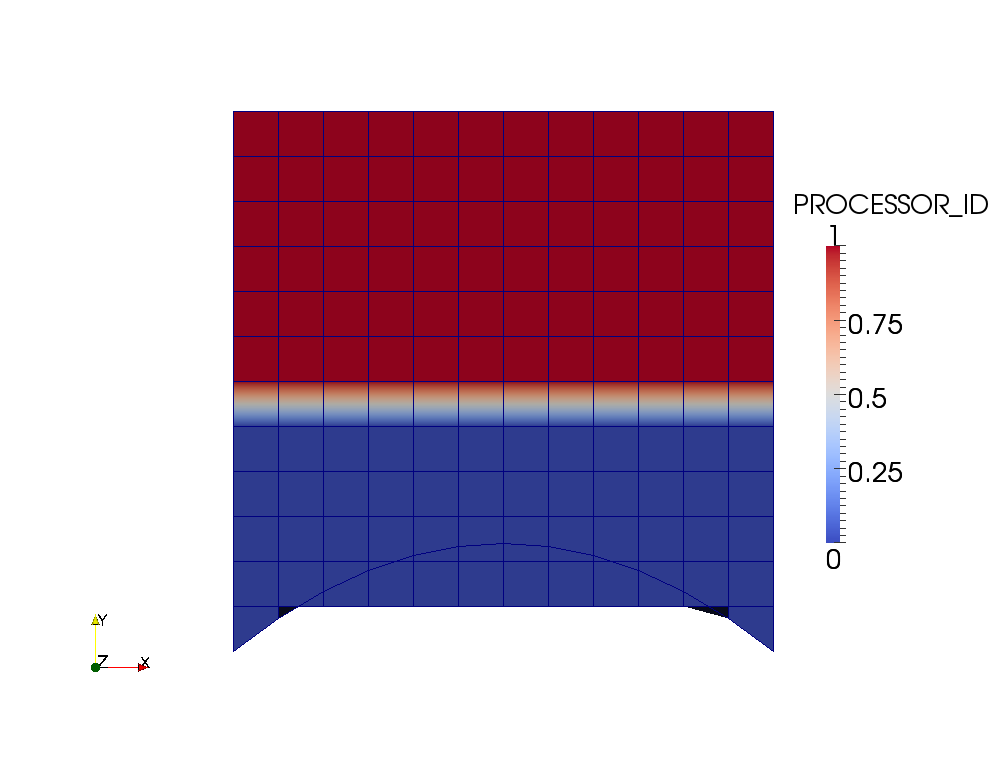
\includegraphics[width=4in]{figures/par-quad-orig}
\caption{Initial, tangled quadrilateral mesh.}
\label{fig:par_quad_orig}
\end{center}
\end{figure*}

\begin{figure*}[htpb]
\begin{center}
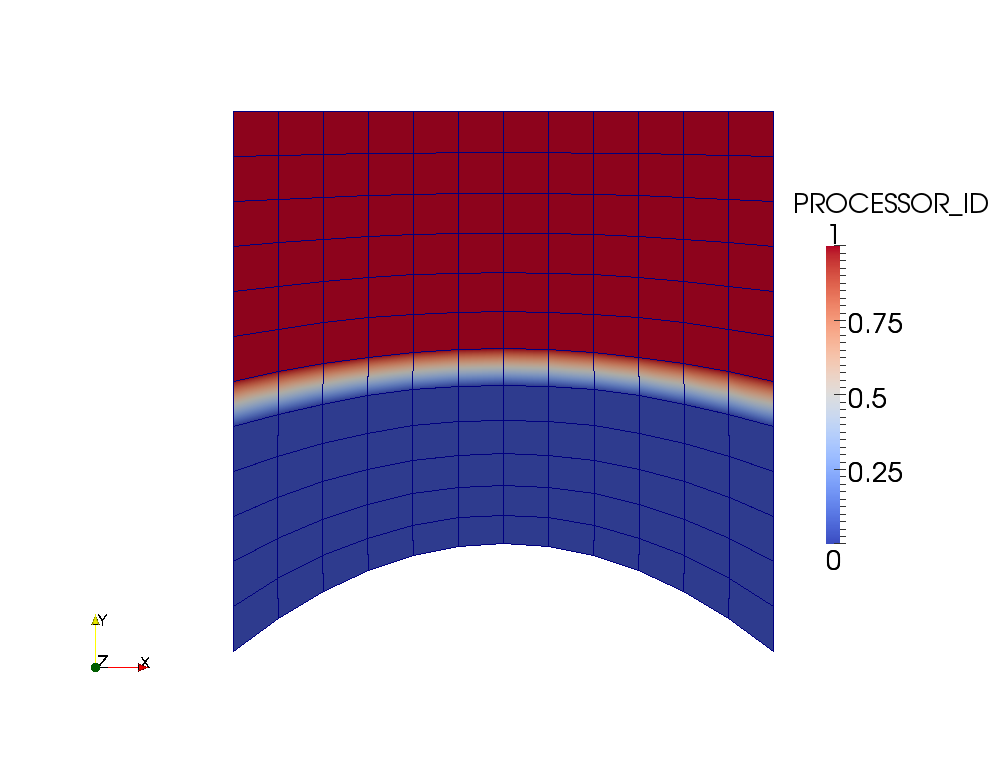
\includegraphics[width=4in]{figures/par-quad-smoothed}
\caption{Untangled and smoothed quadrilateral mesh.}
\label{fig:par_quad_smoothed}
\end{center}
\end{figure*}

\begin{figure*}[htpb]
\begin{center}
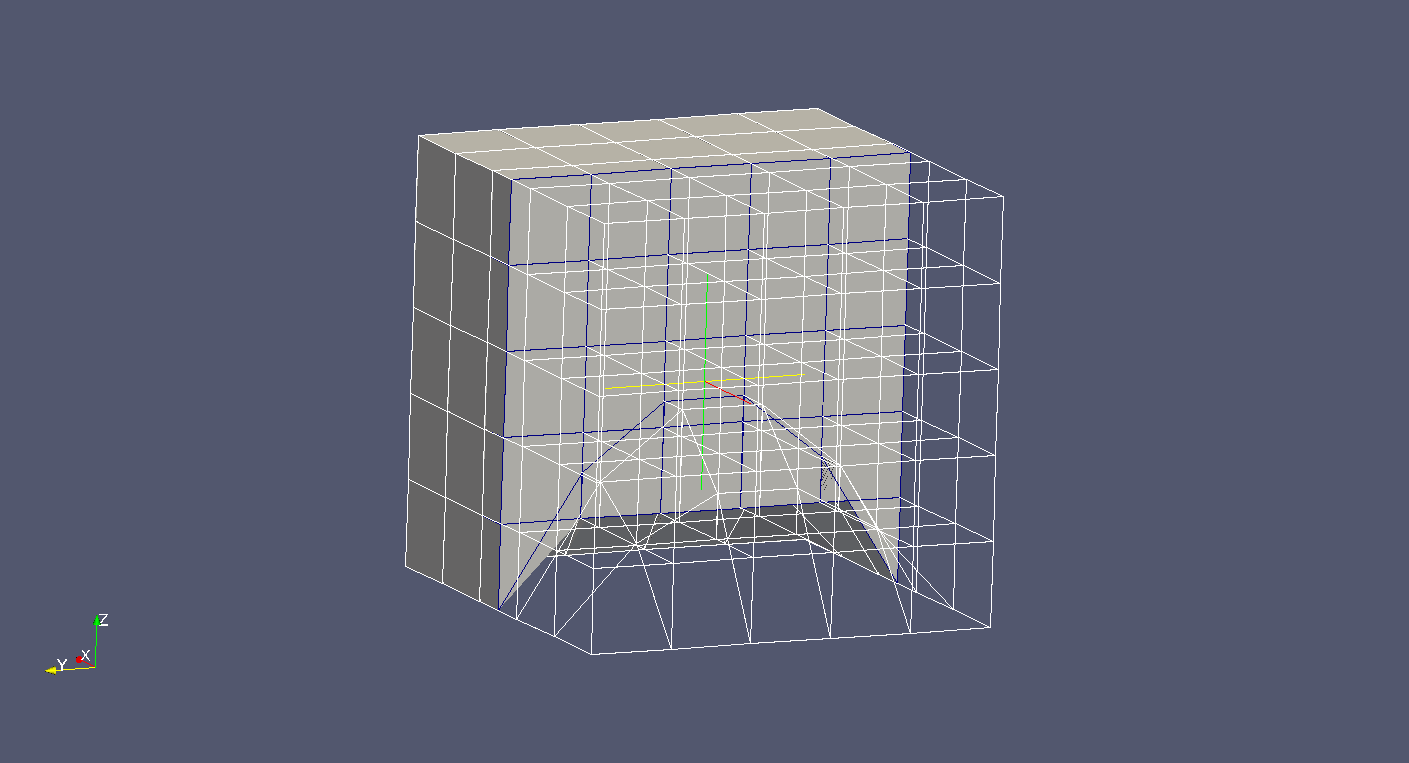
\includegraphics[width=4in]{figures/par-hex-orig}
\caption{Initial, tangled hexahedra mesh.}
\label{fig:par_hex_orig}
\end{center}
\end{figure*}

\begin{figure*}[htpb]
\begin{center}
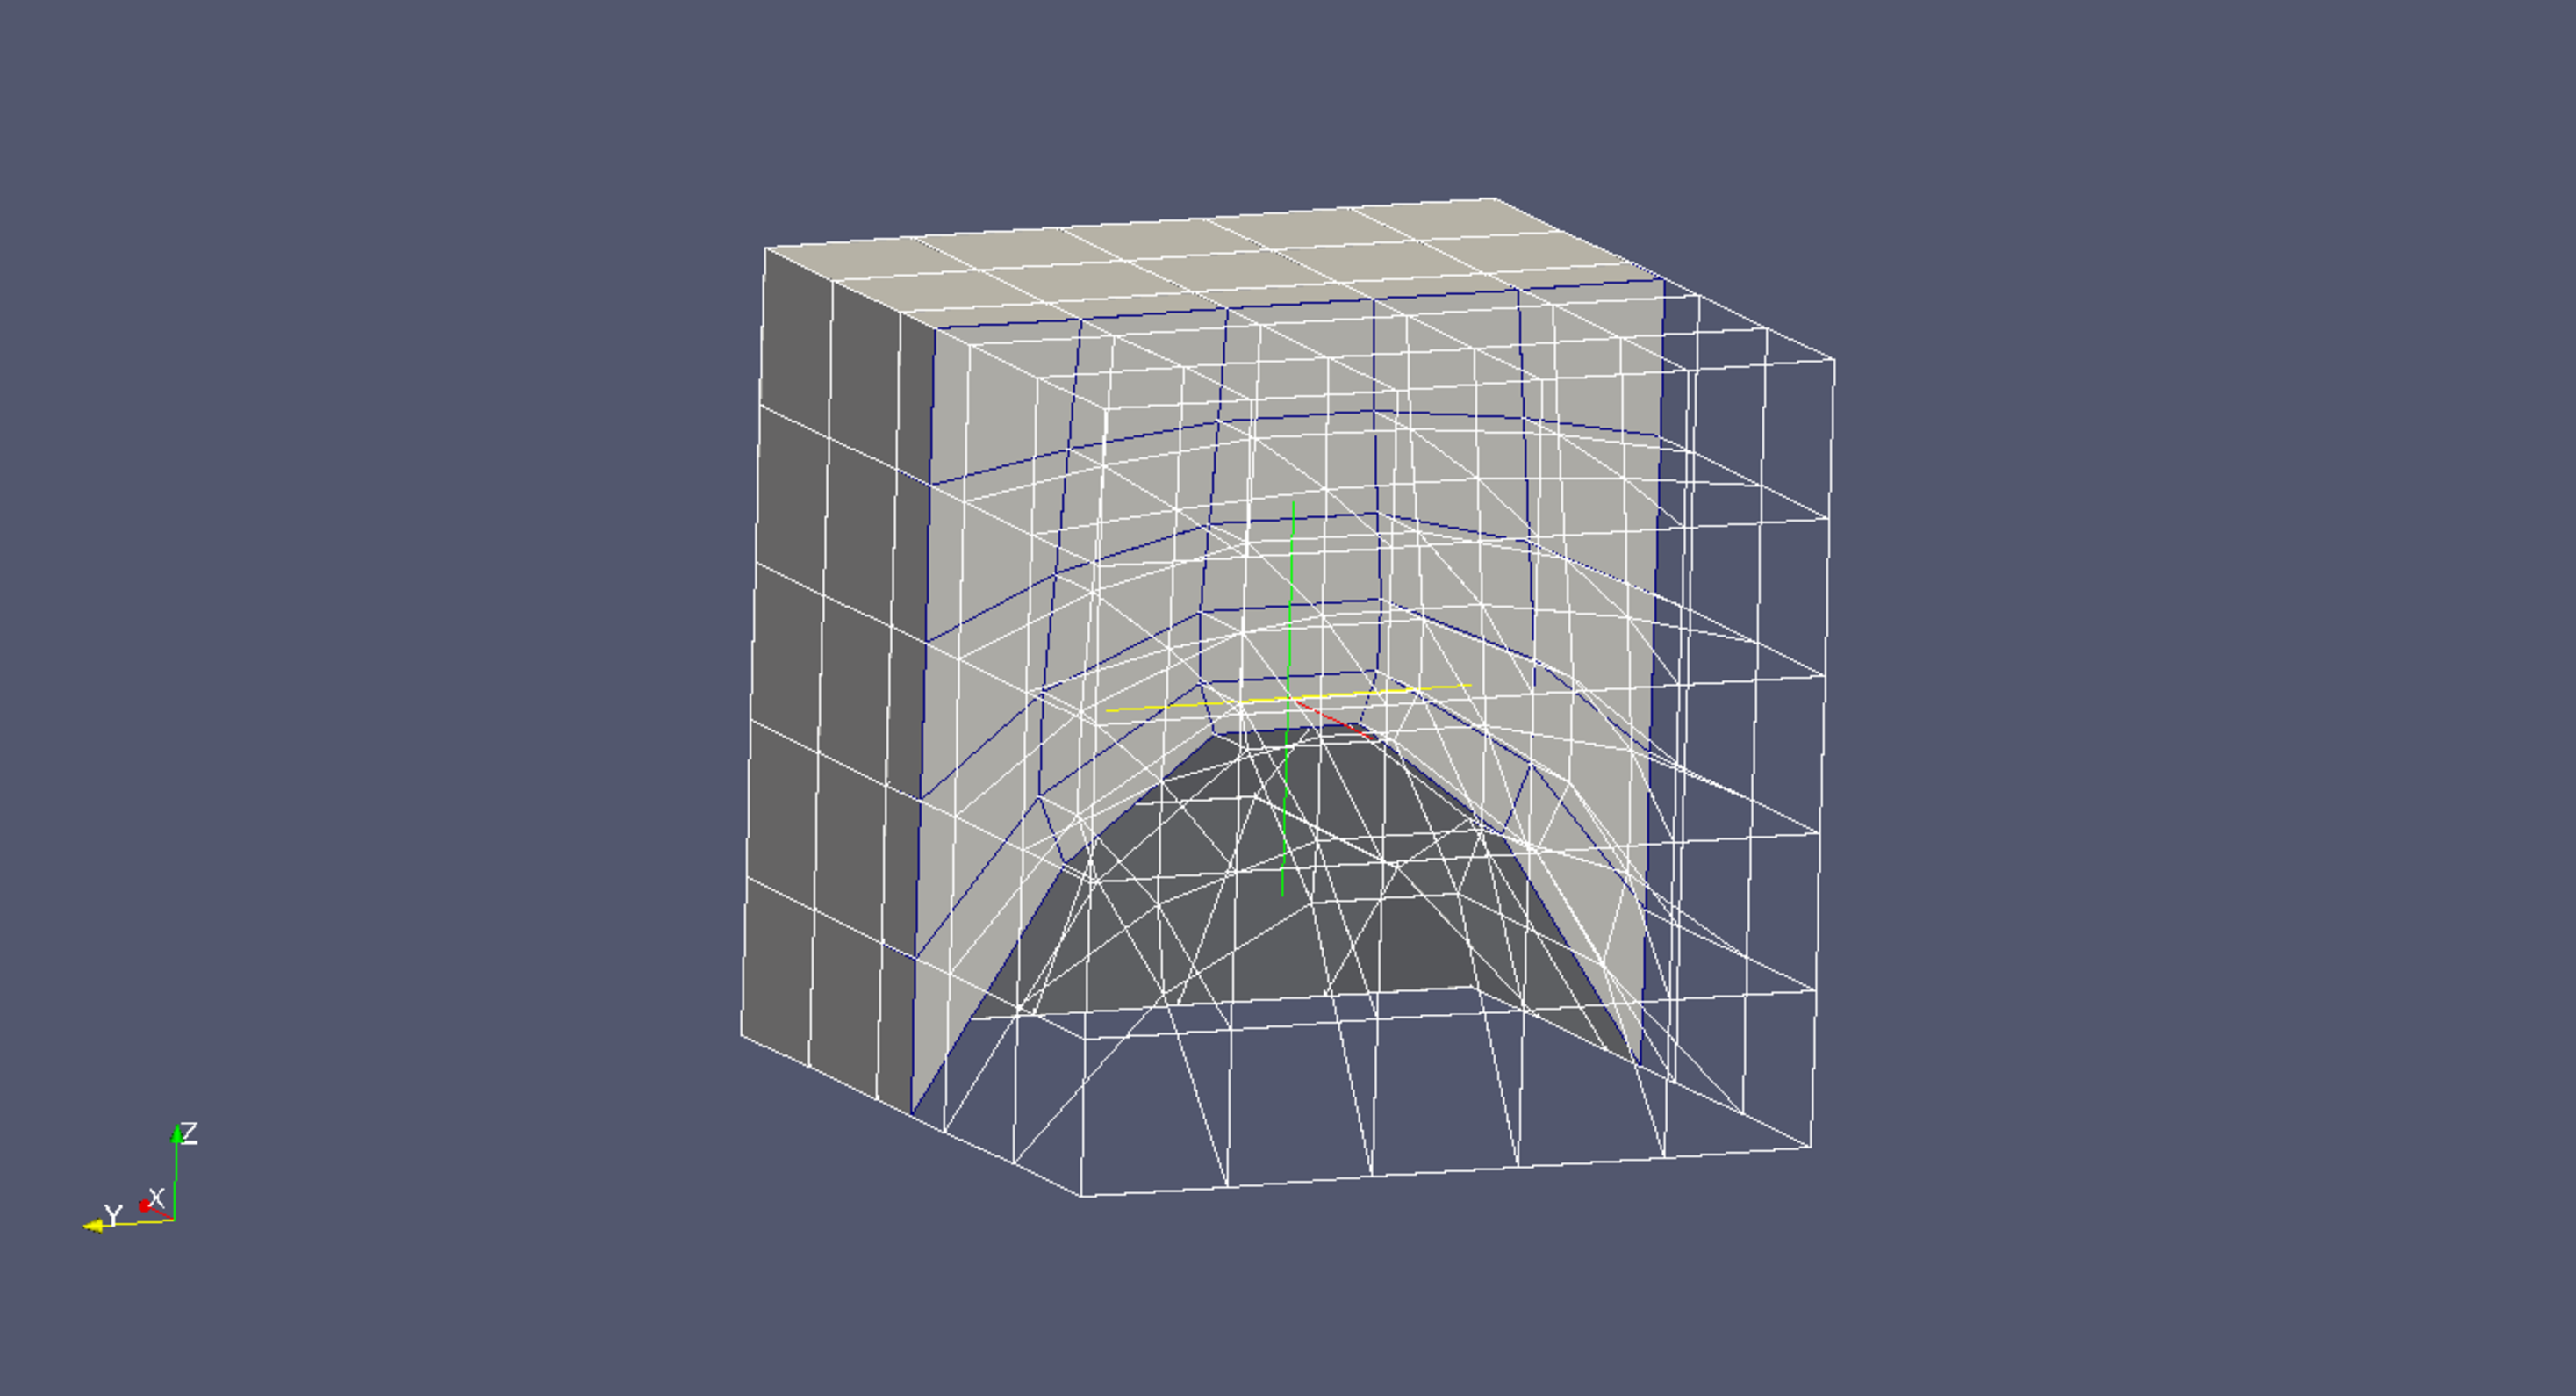
\includegraphics[width=4in]{figures/par-hex-smoothed}
\caption{Untangled and smoothed hexahedral mesh.}
\label{fig:par_hex_smoothed}
\end{center}
\end{figure*}

\subsection{Example: Using \texttt{Mesquite::Mesquite::MsqIMeshP}}

Similar to the example in Section \ref{sec:parallel-example-1}, this example uses the \texttt{LaplaceWrapper} wrapper in parallel to improve element shape.  However, this example assumes that either the iMeshP implementation is partitioning or that it is reading some pre-defined partitioned mesh and it relies on the iMeshP implementation to create ghost elements, assign global vertex IDs, etc.

An implementation of the iMesh and iMeshP APIs must be provided for this example to work.  Mesquite can use these APIs, but does not provide them.

\begin{verbatim}
/* Mesquite includes */
#include <Mesquite.hpp>
#include <MsqIMeshP.hpp>
#include <ParallelMeshImpl.hpp>
#include <ParallelHelper.hpp>
#include <MsqError.hpp>
#include <LaplaceWrapper.hpp>

/* other includes */
#include <mpi.h>
#include <iostream>
using namespace std;

int main( int argc, char* argv[] )
{
  const char input_file[] = "testmesh";
  const char output_file[] = "smoothmesh";

  /* init MPI */
  int rank, nprocs;
  if (MPI_SUCCESS != MPI_Init(&argc, &argv)) {
    cerr << "MPI_Init failed." << endl;
    return 2;
  }
  MPI_Comm_rank(MPI_COMM_WORLD, &rank);
  MPI_Comm_size(MPI_COMM_WORLD, &nprocs);

  /* create a new instance of the iMesh database */
  int ierr;
  iMesh_Instance mesh;
  iMesh_newMesh(NULL, &mesh, &ierr, 0);
  if (iBase_SUCCESS != ierr) return ierr;
  iBase_EntitySetHandle root_set;
  iMesh_getRootSet(mesh, &root_set, &ierr);
  if (iBase_SUCCESS != ierr) return ierr;

  /* create a partition instance in which to read
     the partitioned mesh */
  iMeshP_PartitionHandle partition;
  iMeshP_createPartitionAll(mesh, MPI_COMM_WORLD,
                            &partition, &err);
  if (iBase_SUCCESS != ierr) return ierr;

  /* load mesh */
  iMeshP_loadAll(mesh, partition, root_set, input_file,
                 NULL, &err, strlen(input_file), 0);
  if (iBase_SUCCESS != ierr) return ierr;

  /* create 1 layer of ghost entities */
  iMeshP_createGhostEntsAll(mesh, partition, 3, 1, 1, 0, &err);
  if (iBase_SUCCESS != ierr) return ierr;

  /* create MsqIMeshP instance */
  Mesquite::MsqError err;
  Mesquite::MsqIMeshP parallel_mesh(mesh, partition, root_set,
                                    iBase_REGION, err);
  if (err) {cerr << err << endl; return 1; }

  /* do Laplacian smooth */
  LaplaceWrapper optimizer;
  optimizer.run_instructions(&parallel_mesh, err);
  if (err) {cerr << err << endl; return 1; }

  /* write mesh */
  iMeshP_saveAll(mesh, partition, root_set, output_file,
                 NULL, &ierr, strlen(output_file), 0);
  if (iBase_SUCCESS != ierr) return ierr;

  /* cleanup */
  iMeshP_destroyPartitionAll(mesh, partition, &ierr);
  if (iBase_SUCCESS != ierr) return ierr;
  iMesh_dtor(mesh, &ierr);
  if (iBase_SUCCESS != ierr) return ierr;
  MPI_Finalize();
  return 0;
}
\end{verbatim}


%\chapter{Application Programming Interface (API)} \label{sec:API}

Section \ref{sec:classesRelations} gives the details of the Mesquite paradigm. That section does not
delve into details and should be read before writing a driver code in order to master the basic
concepts. 

Section \ref{sec:detailedAPI} delves into the details of the various concrete classes available in
Mesquite. The syntaxic details of the API are given in the user doxygen doc available by running
'doxygen Mesquite-user.dox' in the directory mesquite/doc/user/doxygen. 

\section{Relations between the Mesquite API Classes} \label{sec:classesRelations}

The Mesquite architecture, shown in Figure \ref{fig:uml}, closely
follows the abstractions of the optimization problem defined in \ref{sec:concepts}.
In particular, the core abstract classes needed to
define a mesh quality improvement algorithm are {\tt QualityMetric},
{\tt ObjectiveFunction} (which takes a {\tt QualityMetric} as
input), and {\tt QualityImprover} (which may take an {\tt ObjectiveFunction}
as input).

Additional classes of importance include:
\begin{description}
\item[QualityAssessor:] to provide information about the
quality of the mesh before or after smoothing to the user or application,
\item[TerminationCriterion:] to customize the stopping criteria
used with a mesh quality improvement algorithm, and
\item[InstructionQueue:] to compose quality improvers and
quality assessors together to form efficient mesh quality improvement
and evaluation methods.
%\item {\tt MeshSet} and {\tt PatchData}: to provide the mechanisms
%for managing the application mesh and geometry information and the
%mesh sub-domains used in optimization procedures.
\end{description}

\subsection{UML Diagram}

\begin{figure*}[htbp]
\begin{center}
    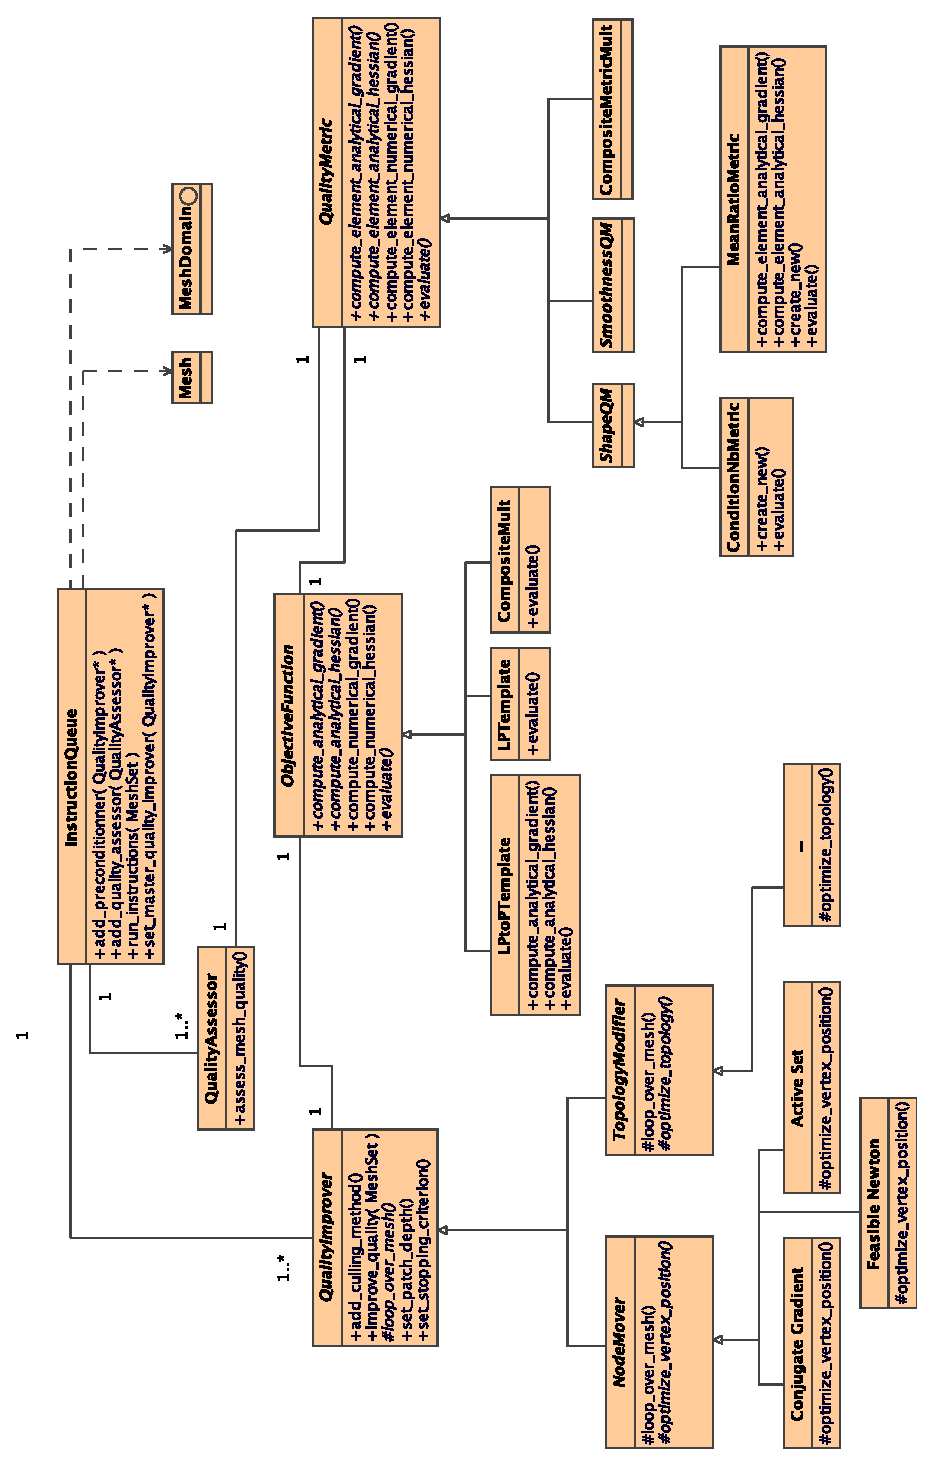
\includegraphics{MesquiteUI.eps}
    \caption{Mesquite user interface UML class diagram.  Abstract
             classes and virtual functions are in italic. Vertical
             links with a triangle indicate inheritance. Plain links
             indicate association. Protected functions are prefixed
             with '\#', public ones with '+' .}
    \label{fig:uml}
\end{center}
\end{figure*}

The UML diagram in figure \ref{fig:uml} presents the layout of the Mesquite classes. It should be
looked over once now, and then examined in more details when each class is described in the
following subsections.


\subsection{The Quality Metric -- Objective Function -- Quality Improver Trio} 
\label{sec:trio}

In the following sections, we will use the notations introduced in section \ref{sec:concepts}. 

Improving a mesh with Mesquite consists mainly in selecting three components: the quality metric,
the objective function template, and the quality improver (i.e. the optimization algorithm). 

The quality metric $q$ describes what the user considers to be a good mesh element as a function of
its vertices' coodinates, and possibly other factors such as its proximity to a boundary or an
equivalent element in a reference mesh. The various quality metrics available are described in
section \ref{sec:QualityMetric} and how to implement a new quality metric is described in section
\ref{sec:QualityMetricImpl}.

Now that the element quality has been defined, a template objective function $f$ (section
\ref{sec:ObjectiveFunction}) must be chosen to formulate the mesh we aim for. For example,
should emphasis be placed on improving the worst elements or on making the mesh
as good as possible in the average. The combination of the
quality metric and the template objective function gives us the mesh quality objective function $F=f
\circ q$.

This mesh quality objective function can now be minimized with an optimization algorithm
(\texttt{QualityImprover}).  The improvement schemes in Mesquite can be divided
into two general catagories.  Vertex movers (subclasses of {\tt VertexMover}) 
change vertex positions to improve the mesh quality.  Topology modifiers (subclasses
of {\tt TopologyModifier}) modify the mesh topology (for example flipping algorithms).
These methods take as input a mesh quality objective function ($F=f \circ q$).
The concrete \texttt{QualityImprover} often acts on an
\texttt{ObjectiveFunction} pointer to retrieve the function value and
gradient $\nabla F$, and sometimes the Hessian ${\cal H} F$, for a certain mesh and concrete \texttt{ObjectiveFunction} /
\texttt{QualityMetric} combination.  Dynamic polymorphism ensures at
runtime that the correct evaluations are performed.


\subsection{Termination Criterion}
\label{termination_section}

Mesquite's \texttt{TerminationCriterion} class contains functionality
to customize the termination of the mesh quality improvement process. 
Mesquite wrappers (section \ref{sec:wrappers}) already have an embedded default termination
criterion. The termination criterion provides an automatic mechanism to stop an optimization
procedure. An example of a termination criterion is stopping the quality
improvement when the objective function gradient norm is close
to zero in a non-linear programming problem. Many other criteria are available in Mesquite (see
section \ref{sec:TerminationCriterion}).  Generally, when using the
detailed API, termination criteria have to be set in order for the
quality improver to terminate, although some \texttt{VertexMover}s
provide default criteria which are used if the user does not
explicitly set the \texttt{TerminationCriterion}.
 

\subsection{Quality Assessors}

Mesquite's \texttt{QualityAssessor} class encapsulates functionality to
evaluate quality metric values for a given mesh, to accumulate
statistical information about those values, and to report that data to
the user or the calling application.  In particular, a \texttt{QualityAssessor}
object takes a {\tt QualityMetric} class as input to evaluate a given mesh and then
reports information like the maximum, average, and standard deviation
of those values.

% \subsection{Culling Capabilities} \label{sec:culling}
% Mesquite includes methods called {\it culling} schemes
% which are intended to decrease the time it takes for the
% quality improvers to reach an adequate mesh.  These schemes
% the mporarily fix the positions of certain vertices which
%satisfy a given culling criteria.  These fixed vertices
%are said to be {\it culled} from the optimization procedure.
%This reduces the number of variables in the optimization
%problem, and therefore this modified problem can often
%be solved in significantly less time than the original problem.  
% LAF - there are no details here - it's not worth including as is

%\subsection{Mesh Data Classes} \label{sec:MeshData}
%There are two mesh data classes in Mesquite, \texttt{MeshSet} and
%\texttt{PatchData}, which have been designed to meet two different
%needs.  The {\tt MeshSet} class is a container that holds pointers, or
%handles, to the meshes provided by the application.  It also provides
%the mechanisms necessary to obtain the mesh information from the
%application through a well-defined, flexible API (see Section
%\ref{sec:meshset}).  To minimize the memory footprint of the Mesquite
%library, only detailed information for the optimization procedure
%subdomains is stored at any given time in the {\tt PatchData} class.
%One or more {\tt PatchData} objects can be originated from the {\tt
%MeshSet} object, and {\tt PatchData} obtains detailed mesh
%information, such as vertex coordinates and element connectivity,
%through the MeshSet accessor functionality.  The \texttt{PatchData}
%class makes Mesquite scalable in that prohibitive memory costs
%associated with making a copy of a large application mesh can be
%avoided by dividing the mesh into patches on which to perform the
%optimization sequentially.
%\subsubsection{MeshSet Interactions with Application Meshes}
%\label{sec:meshset}
%\subsubsection{PatchData Interactions with QualityImprovers}
%Quality improvers are written to relocate nodes or modify topology
%within a \texttt{PatchData}, without any need to know whether the
%\texttt{PatchData} corresponds to the whole mesh or a subset of
%it. The \texttt{PatchData} information is generated by the
%\texttt{MeshSet} class with the \texttt{get\_next\_patch} function ---
%the equivalent of an iterator over a series of patches covering the
%mesh.  The user can set Mesquite to use different types of
%\texttt{PatchData}, ranging from a patch of elements containing one
%particular vertex to a patch of vertices connected to a central vertex
%through edges or a unique patch that covers the whole MeshSet
%(recall that this could be the union of several meshes added by the
%application to \texttt{MeshSet}).

%\texttt{PatchData} and its associated classes
%(e.g. \texttt{PatchDataVerticesMemento}) provides much functionality
%to the optimization algorithms.  Memento patterns can remember the
%state of a \texttt{PatchData} geometry or topology at a given
%iteration and restore the \texttt{PatchData} to that state
%later. Simple functions can move the \texttt{PatchData} $n$ vertices
%in a direction $d \in \Bbb{R}^{3n}$ while constraining the boundary
%vertices to their geometrical surface.

\subsection{The Instruction Queue} \label{sec:IQ}

The \texttt{InstructionQueue} class allows a sequence of operations
such as quality assessment and quality improvement to be performed on
a \texttt{MeshSet} object. The \texttt{InstructionQueue} 
provides a convenient framework to shield the user
from the algorithm syntax and to ensure a consistent use of the
Mesquite capabilities.  One or more quality improvers can be
associated with an {\tt InstructionQueue}, but one must be designated
as the {\it master} quality improver that determines the ultimate 
improvement goal.  All progress made by Mesquite will be
measured against the quality metrics set in the master quality
improver.  To improve the effectiveness and efficiency of the mesh
quality improvement process, several quality improvers can be used as
``pre-conditioners'' for the master quality improver.  For example, a
user may precede an optimization-based master quality improver with a
mesh untangler and/or Laplacian smoothing.  Once an
InstructionQueue has been defined, a single call to \texttt{run\_instructions} 
will perform all the contained operations.  We note
that once an \texttt{InstructionQueue} has been defined, it can be used
for several \texttt{MeshSet} objects.


Some predefined \texttt{InstructionQueue} objects, called \emph
{wrappers}, are available for high-level or novice users.  See
section \ref{sec:wrappers} for more detailed information on wrappers.
%mbrewer: removing these sentences because the next section goes
%in depth into wrappers
%Those
%typically consist of a quality assessor, followed by a mesh
%pre-conditioner such as an untangler, followed by a master quality
%improver, and finally another quality assessor.


\section{Wrappers}
\label{sec:wrappers}
To improve meshes with a minimum of Mesquite function calls, we have 
provided a set of wrapper classes that encapsulate the 
most commonly used combination of quality metrics, improvement
algorithms and stopping criterion. Essentially, the wrappers are
inherited from the InstructionQueue, setting in their constructors
which algorithms to call. Using these wrappers, only
two lines of code are required to improve a \texttt{MeshSet}.

Wrappers do not generally provide access to low-level features such
as setting a specific termination criterion.  While some wrappers do allow
users to adjust specific parameters, the ability to customize the wrapper
is limited.

\subsection{The Shape Improvement Wrapper}
\label{sec:ShapeImprovementWrapper}
The \texttt{ShapeImprovementWrapper} class 
first uses the inverse mean ratio quality
metric (section \ref{sec:QualityMetric}) to assess and report
the quality of the mesh elements. It then untangles the mesh, if
necessary, and reports the quality of the mesh after
the untangle step.  It then improves the mesh with the
feasible Newton algorithm applied to the composition of the mean ratio
quality metric with the $\ell_2^2$ objective function
(section \ref{sec:ObjectiveFunction}). Finally, the quality of the final
mesh is assessed and reported. 


\section{Detailed Application Programming Interface}
\label{sec:detailedAPI}

\subsection{Quality Metric} \label{sec:QualityMetric}

%{\it 
%What is a quality metric? Define full range, acceptable range, what it means 
%if the metric uses a map, nodal-invariance, well-posed metrics, averaging 
%methods, sample points. Give a list of the individual metrics we support. 
%Provide a key to the tables.
%}

\subsubsection{Concept}

In Mesquite, the \texttt{QualityMetric} class provides a measure of
the quality of individual mesh entities.  Quality metrics can evaluate
either element quality (for example, the mean ratio quality
metric provides a measure of element shape quality) or vertex quality
(for example, the sum of the adjacent edge lengths squared provides a
measure of vertex smoothness).  

In addition to the quality metric function value, the {\tt
QualityMetric} class also provides the gradient and Hessian
information needed for many optimization algorithms.  Numerical
approximations of the gradient and Hessian are automatically provided
by the \texttt{QualityMetric} base class.  QualityMetric implementations
may can optionally
implement analytical expressions for the gradient and Hessian, which are 
typically more computationally efficient and accurate.  For example, the
mean ratio
quality metric implementation provides an analytic calculation of the gradient 
that is approximately twice as fast as the numerical solution, and an analytic
calculation of the Hessian that is almost five times as fast as the
numeric approximation.  The
cost of implementing the analytical gradients and Hessians can often
be alleviated by the use of automatic differentiation tools
(for example, \cite{bischofadic}).

Mesquite also allows the user to scale metric values or combine
multiple metrics together to form a composite metric.  However, only
metrics which are evaluated on the same type of mesh entity can be
composed together.  That is, Mesquite does not allow element-based
metrics and vertex-based metrics to be added or multiplied together
because the result is not a meaningful measure of either element or
vertex quality.

\subsubsection{Currently Available Quality Metrics}  
Quality metrics within
Mesquite are grouped by the type of mesh properties that they measure.
Currently, there are four property groups: shape, smoothness, volume,
and untangle.  Composite metrics which allow the user to combine
multiple metrics or to scale metrics are given a separate group,
composite.  Future Mesquite development will include the
implementation of metrics falling under other group headings such as
orthogonality, shear, and alignment.  Table \ref{current-metrics}
lists the quality metrics currently available within Mesquite.  For
detailed definitions of the metrics, see \cite{Kn01}.  We note that
the implementation of the mean ratio metric has been extensively
optimized, and analytical gradients and Hessians are available for
that function.  Many other metrics currently use numerical gradients and
Hessians.

The two composite metrics which are currently implemented
allow users to either multiply two metrics' values
together or raise a single metric's value to a given power.
The latter allows for negative powers and can therefore be used
to obtain the inverse of any Mesquite quality metric.  

\begin{table}[!hp]
\begin{center}
\begin{tabular}{|l|c|c|c|c|c|c|}
\hline
Name               & Group      & Tri/Tet & Quad/Hex & Feasibility & Analytic  \\
                   &            &         &          & Region      & Gradient \\
                   &            &         &          &             & and Hessian   \\  
\hline
Area Smoothness    & Smoothness & Yes     & Yes      & No          & No    \\
Aspect Ratio       & Shape      & Yes     & No       & No          & No    \\
Cond. Num.         & Shape      & Yes     & Yes      & Yes         & No    \\
Corner Jacobian    & Volume     & Yes     & No       & No          & No    \\
Ideal W. Inv. Mean & Shape      & Yes     & Yes      & Yes         & Yes   \\
Ideal W. Mean Ratio& Shape      & Yes     & Yes      & Yes         & Yes   \\
Untangle Beta      & Untangle   & Yes     & Yes      & No          & No    \\
\hline
\end{tabular}
\label{Element Metrics}
\caption{List of the element-based quality metrics provided with Mesquite.}
\end{center}
\end{table}

\begin{table}[!hp]
\begin{center}
\begin{tabular}{|l|c|c|c|c|c|c|c|}
\hline
Name               & Group      & Tri/Tet & Quad/Hex  & Feasibility & Analytic  \\
                   &            &         &           & Region      & Gradient   \\
                   &            &         &           &             & and Hessian   \\  

\hline
Edge Length        & Smoothness & Yes     & Yes       & No          & No         \\
Edge Length Range  & Smoothness & Yes     & Yes       & No          & No         \\
Local Size         & Volume     & Yes     & Yes       & No          & No         \\
Vert. Cond. Num.   & Shape      & Yes     & Yes       & Yes         & No         \\
\hline
\end{tabular}
\label{Vertex Metrics}
\caption{List of the vertex-based quality metrics provided with Mesquite.}
\end{center}
\end{table}

\begin{table}[!hp]
\begin{center}
\begin{minipage}[h]{\textwidth}
\renewcommand{\thempfootnote}{\arabic{mpfootnote}}
\begin{tabular}{|l|c|c|c|c|}
\hline
Name                   & Tri/Tet & Quad/Hex  & Feasibility & Analytic  \\
                       &         &           & Region      & Gradient  \\
                       &         &           &             & and Hessian   \\  
\hline
I DFT Generalized      & Yes     & Yes       & Yes or No
\footnote{The generalized version
of the I DFT metric contains parameters which can be modified by the user.  For certain
values of these parameters, the metric will require the corner of the mesh to be within a
feasibility region.  For other values of these parameters, the metric will not have this
requirement.}
                                                           & Yes       \\
I DFT Inv. Mean Ratio  & Yes     & Yes       & Yes         & Yes       \\
I DFT No Barrier       & Yes     & Yes       & No          & Yes       \\
I DFT Strong Barrier   & Yes     & Yes       & Yes         & Yes       \\
I DFT Weak Barrier     & Yes     & Yes       & Yes         & Yes       \\
RI DFT                 & Yes     & Yes       & Yes         & Yes       \\
sI DFT                 & Yes     & Yes       & Yes         & No        \\
sRI DFT                & Yes     & Yes       & Yes         & No        \\
\hline
\end{tabular}
\label{Corner Metrics}
\caption{List of the target-based quality metrics provided with Mesquite.}
\end{minipage}
\end{center}
\end{table}

\begin{table}[!hp]
\begin{center}
\begin{tabular}{|l|c|c|c|}
\hline
Name        & Operation        & Analytic Gradient & Analytic Hessian \\
\hline
Add         & $q_1 + q_2$      & No                & No               \\
Mupliply    & $q_1 \times q_2$ & No                & No               \\
Power       & $q_1^s$          & No                & No               \\
Scalar Add  & $q_1 + s$        & No                & No               \\
Scalar Mult.& $q_1 \times s$   & No                & No               \\
\hline
\end{tabular}
\label{Composite Metrics}
\caption{List of the quality metrics for combining or modifying other quality metrics.}
\end{center}
\end{table}


\begin{table}[h]
\begin{center}
\begin{minipage}[h]{\textwidth}
\renewcommand{\thempfootnote}{\arabic{mpfootnote}}
\begin{tabular}{|l|c|c|c|c|c|}
\hline
Metric Name        & Type       & Full Range  & Ideal \footnote[1]{The value of this metric
for the ``ideally'' shaped element ({\it e.g.} an equilateral triangular element).}
                                                      & Degenerate  \footnote[2]{The value of this metric
for a degenerate element ({\it e.g.} a triangular element with co-linear points).}
                                                                    & (Default) \\
                   &            &             &       &             & Averaging\\
\hline
Inverse Mean Ratio & Shape      &$[1,\infty]$ & 1     & $\infty$    & LINEAR\\ 
Mean Ratio         & Shape      &$[0,1]$      & 1     & 0           & LINEAR\\ 
Condition Number   & Shape      &$[1,\infty]$ & 1     & $\infty$    & LINEAR\\ 
Untangle  Beta     & Untangle   &$[0,\infty]$ & 0\footnote[3]{The untangle beta metric will
have a positive value for a degenerate element and for some non-inverted elements with a small
area or volume.  It will have a value of zero for non-inverted elements, including the ``ideally''
shaped element, as long as those elements have sufficiently large area or volume.}
                                                      & $\alpha : \alpha > 0$ \footnotemark[3]
                                                                    & R.M.S.\\ 
\hline
\end{tabular}
\caption{\label{QualityMetrics1} Mesquite Quality Metrics Summary}
\end{minipage}
\end{center}
\end{table}

\noindent {\bf Mean Ratio Metric} \newline
Give description, formulas. 

\subsubsection{Composite Metrics}

\subsection{Objective Function} \label{sec:ObjectiveFunction}

\subsubsection{Concept}
Remember the notations introduced in section \ref{sec:concepts}:
for each element of the mesh, let there be an associated quality metric, 
$q_n$.  Define the vector 
\begin{equation}
Q = [ q_1, q_2, \ldots, q_n ]
\end{equation}
where $N$ is the number of elements in the mesh. \footnote{For vertex-based metrics, an equivalent vector can be defined for a
quality metric associated with each free vertex $(1 \dots M)$ in the mesh. An example of vertex-based
metric is the longest edge connected to a vertex.}

While the \texttt{QualityMetric} class provides a way to evaluate the
properties of individual mesh entities, the \texttt{ObjectiveFunction}
class provides a way of combining those values into a single number
for the domain of the optimization problem.  This domain can either be
the entire mesh or a sub-mesh containing a subset of the free vertices.
For example, one available objective function template $f$ is the $\ell_{2}^2$
function which is the standard $\ell_{2}$ vector norm squared.  
Given an element-based quality metric $q$ and a mesh sub-domain $E$, the mesh 
quality objective function $F$ would be the composition of the template
objective function and the quality metric function 
\begin{equation}
F({\bf x}) = f \circ q({\bf x}) = \sum_{i \in E} (q_i({\bf x}))^2 \;\; .
\end{equation}

Given a \texttt{QualityMetric} $q$ and a mesh sub-domain $E$, the
\texttt{ObjectiveFunction} derived class computes the value of 
$F$ and, for $f$ and $q$ satisfying the appropriate smoothness
conditions, the mesh quality objective function's gradient and Hessian
with respect to the vertex positions.  As with {\tt QualityMetric},
Mesquite allows the gradient of $F$ to be calculated either
analytically or numerically. Computing the gradient of $F$
numerically is computationally expensive but requires only the quality
metric values.  If the gradient is calculated analytically, the
first derivative of the template objective function $f'$ and the
quality metric gradient $\nabla q$ are both required.\footnote{The 
quality metric gradients $\nabla q$ can be provided either numerically 
or analytically.}
To obtain the gradient $\nabla F$, the chain rule is applied
\begin{equation}
\nabla F({\bf x}) = \amalg_{i \in E} \left[ \nabla q_i({\bf x}) 
 (f' \circ q({\bf x}) ) \right] \;\; ,
\end{equation}
where $ f' \circ q({\bf x})$ is a scalar and $\amalg_{i \in E}$ denotes the
assembly over all the elements or vertices, for element-based or 
vertex-based quality metrics respectively.
Due to the significant advantages in computational
cost, analytical gradients have been implemented for all of the
continuously differentiable template objective functions in Mesquite.
Furthermore, an analytical Hessian calculation has been implemented
for the $\ell_p^p$ template objective function.  

\begin{table}[htb]
\begin{center}
\begin{tabular}{|c|c|c|}
\hline
Function & Gradient & Hessian\\
\hline
$\ell_P^P$     & Ana./Num.&Ana.\\
%$\ell_P$       & Ana./Num.& Not Avail.\\
$\ell_{\infty}$& Not Avail.& Not Avail.\\
Comp. Add      & Ana./Num.& Not Avail.\\
Comp. Mult.    & Ana./Num.& Not Avail.\\
Scalar Add     & Ana./Num.& Not Avail.\\
Scalar Mult.   & Ana./Num.& Not Avail.\\
\hline
\end{tabular}
\label{current-objfunc}
\caption{List of the current objective functions available within
Mesquite.  With each function is a description of the types of
gradient and Hessian information available (Analytical and/or Numerical
or Not Available).}
\end{center}
\end{table}

\subsubsection{Available Objective Functions}

%\noindent {\bf The $\ell_p$ Template} \newline
%Given $1 \leq p < \infty$, let
%\begin{equation}
%\| Q \|_p = ( \sum_{n=1}^N \mid q_n \mid^p )^{1/p}
%\end{equation}
%be the $\ell_p$ template objective function. We recommend using the next template, \
%$\ell_p^p$ since the $\ell_p$ template has no analytical gradient / Hessian implemented in Mesquite.\newline

\noindent {\bf The $\ell_p^p$ Template} \newline
Given $1 \leq p < \infty$, let 
\begin{equation}
\| Q \|_p^p = ( \sum_{n=1}^N \mid q_n \mid^p )
\end{equation}
be the 
$\ell_p^p$ template. The $\ell_p^p$ Template has its analytical gradient and Hessian implemented in
Mesquite. With $p=1$, this is the ``workhorse'' template objective function in Mesquite when the \emph{average}
quality of the mesh is to be improved. Increasing the value of $p$ will put more weight in improving
the quality of the worst elements. 
\newline

\noindent {\bf The $\ell_{\infty}$ Template} \newline
The $\ell_{\infty}$ template is
\begin{equation}
\| Q \|_{\infty} = \max_{n=1,\ldots,N} \mid q_n \mid
\end{equation}


\subsection{Composite Objective Functions}

Mesquite has four composite objective functions.  These are
\texttt{CompositeOFAdd}, \texttt{CompositeOFMultiply}, \texttt{CompositeOFScalarAdd}, and
\texttt{CompositeOFScalarMultiply}.  This combination allows users
to combine two objective functions by adding or multiplying
their respective values or to adjust a single objective function
by adding a scalar value or by multiplying by a scalar value.  
The user can adjust the objective function to modify the
optimization problem or to make the objective function value
more easily interpreted.  Scaling objective function values
is often useful when using a termination criterion based on the
objective function values. Unlike the quality metrics, 
two objective functions can be combined
even if the underlying quality metrics are defined on different entity
types.  That is, an objective function which operates on a vertex-based
quality metric can be added to an objective function which operates
on an element-based quality metric.  This structure allows the user
to have the maximum flexibility in defining an objective function with
which to measure the quality of a mesh.  Analytic gradients and
Hessians have not been implemented for the composite objective
function templates in Mesquite.

%\begin{verbatim} analytic gradients / Hessians ??? \end{verbatim} 

\subsection{Vertex Mover} \label{sec:VertexMover}

\subsubsection{Concept}
There are two quality improver base classes in the Mesquite architecture: \texttt{VertexMover} and
\texttt{TopologyModifier}. VertexMovers have the ability to relocate optimally the mesh vertices,
given a quality metric and a template objective function, without changing the mesh topology.
One important aspect of vertex movers is
the ability to seamlessly perform an optimization of a whole mesh or
to perform a sequence of optimizations on sub-patches of the mesh.
This behavior is chosen by the user at the \texttt{QualityImprover}
level with the \texttt{set\_patch\_type} function. 

\subsubsection{Available Vertex Movers}

\begin{table}[h]
\begin{center}
\begin{tabular}{|l|c|c|c|c|c|}
\hline
Solver Name & Description & Templates & L/G & Num/Anal & Fixed Vertices? \\ \hline
Steepest Descent & Classical & $\ell_p$ & Both & Both & Yes \\
Conjugate Gradient & & & & & \\
Feasible Newton & & & & & \\
Active Set & & Own & & & \\
Laplace & & None & & & \\
Randomize & & None & & & \\
\hline
\end{tabular}
\caption{\label{Solvers} Mesquite Solver Summary}
\end{center}
\end{table}

{\bf Conjugate Gradient Algorithm } \newline
\label{append_conjgrad}
This algorithm requires only
the objective function value $F$ and the objective function gradient $\nabla F$. 
In Mesquite this is usually done by applying the chain rule to the
analytical gradient of the objective function given the numerical or
analytical gradients of the element (or vertices) quality metrics 
(example given in section \ref{sec:ObjectiveFunction}). 

The conjugate gradient algorithm
has a linear convergence property for most problems. By using the
Polak-Ribi\`ere scheme to select a search direction which is a
combination of the gradient at the current iteration with the gradient
from one or more previous iteration, it avoids the zigzagging behavior
exhibited by the steepest descent algorithm when the equal cost
surfaces of the objective function are elongated (e.g. in narrow
valleys). In Mesquite this algorithm can be used with mesh patches of
any size; thus it is appropriate for optimizing all node positions 
simultaneously for any combination of $C^1$ objective functions and
quality metrics (see \cite{FeasNewt} for more details). 

Conjugate gradient is memory efficient but converges slowly.
The conjuguate gradient algorithm is a lot slower than the Feasible Newton algorithm
when analytical gradient and hessians are available for the quality metrics. On the other hand, the
memory footprint of the conjugate gradient algorithm is a lot smaller than for the feasible Newton 
algorithm, since no Hessian has to be stored. A rough estimate would be a memory 
footprint 2 times smaller for a tetrahedral mesh, and 8 times smaller for an hexahedral mesh.  
\newline

{\bf Feasible Newton Algorithm } \newline
\label{append_feasnewt}
Newton's method minimizes a quadratic
approximation of a non-linear objective function. The algorithm requires
the objective function value, its gradient, \emph{and} its Hessian information.
Again, in Mesquite this
is usually done by computing the analytical gradient and Hessian of
the objective function given the numerical or analytical gradients and
Hessians of the quality metrics.  Note that objective functions that
lead to non-sparse Hessians entail a prohibitive memory cost in
Mesquite.\footnote{$\ell_p$ for $p \geq 2$ is such a function. The
number of variables in the objective function is the number of degrees
of freedom of the mesh, which must be squared to obtain the number of
entries in a dense Hessian.}  Newton's method is known to converge
super-linearly near a non-singular local minimum.   
Mesh-optimization problems that are performed within the neighborhood of
the minimum are a perfect application for Newton's method. In
Mesquite this algorithm can be used with mesh patches of any size,
making it appropriate to optimize all vertex positions simultaneously
for any $C^2$ objective function with a sparse Hessian.  In practice,
users will often observe an order of magnitude improvement\footnote{The larger the mesh, the
more dramatic the speed improvement between conjugate gradient (linearly convergent) and feasible
Newton (super-linearly convergent).} in
computation time when using the feasible Newton algorithm instead of
the conjugate gradient algorithm, making feasible Newton a worthwhile
choice when applicable (see \cite{FeasNewt} for more details). \newline

{\bf Active Set Method } \newline
\label{append_activeset}
The active set algorithm has been
developed for non-continuously differentiable objective functions such
as those computing the maximum value of a quality metric within a
patch of elements. This method is based on a non-smooth steepest
descent algorithm which efficiently computes a search direction and
step size based on the gradients of the values contained in the active
set.  Currently, this algorithm works on a patch of triangular or 
tetrahedral elements that 
contain a single free vertex.  Repeated
sweeps over the free vertices in the mesh leads to overall mesh
improvement (see \cite{fp:ijnme00} for more details).

\subsection{Topology Modifier} \label{sec:TopologyModifier}

Topology modifiers are the second type of quality improvers, They allow for optimal topology
modifications of the mesh , using swapping, flipping, etc ... 

Not available at this time. 

\subsection{Termination Criteria}
\label{sec:TerminationCriterion}
\subsubsection{Concept}
With the exception of wrappers (section \ref{sec:wrappers}), Mesquite algorithms need to be told
when to stop iterating within a given optimization procedure. 
As mentioned previously, many quality improvement algorithms can
perform mesh optimization on either the global mesh or on sub-meshes.
In the later case, the algorithm must be capable of determining when
to terminate two processes: 1) the optimization on the sub-mesh and 2)
the looping over the sub-meshes.  Mesquite's
\texttt{TerminationCriterion} class has been designed to handle either
of these cases.  Therefore, in general, quality improvers use two
\texttt{TerminationCriterion} objects: one, called the {\it inner
criterion}, to terminate the optimization of the sub-mesh and
another, called the {\it outer criterion}, to terminate the looping
over the sub-meshes.  Typically, quality improvers that support both
local and global optimizations always use two termination criterion. 
The outer criteria is set to terminate the optimization process after
one iteration in the global case.

Note that an interrupt handler (SIGINT) is also available, see section \ref{sec:Ctrl-C}. 

\subsubsection{Available Termination Criteria}
A wide range of cost, quality, 
and progress-centric termination
criterion types have been studied. These criteria have two basic types - 
absolute or relative - depending on whether or not the criterion is scale 
dependent.  Fourteen of these have been
implemented in \texttt{TerminationCriterion}.  Among the implemented
types are criteria which terminate optimization procedures due to
exceeding a set number of iterations, exceeding an allotted amount of
time, or reaching a mesh with a sufficiently small objective function
gradient.  

Any combination of the available criteria can be set on a given
\texttt{TerminationCriterion} object with the \texttt{add\_criterion\_type\_with\_double} and 
the \texttt{add\_criterion\_type\_with\_int} functions.  Compound criteria types consist
of statements joined by 'OR', for which 
the optimization process will be terminated when {\it any} of
the criteria have been satisfied.\footnote{Currently we have found little use
for compound criteria joined by 'AND', but this also could be implemented.}

The \texttt{TerminationCriterion} object is then set on the \texttt{QualityImprover} concrete class
with the \texttt{set\_inner\_termination\_criterion} and the \texttt{set\_outer\_termination\_criterion}
functions. Note that setting an inner or outer criterion on a \texttt{QualityImprover} overwrites
the previous inner or outer criterion.

The list of available termination criteria follows; those are the possible value of the
\texttt{TCType} enum. Make sure to consult the doxygen documentation
in mesquite/doc/user/doxygen for a list up to date with your Mesquite release. 
\begin{description}
\item[GRADIENT\_\-L2\_\-NORM\_\-ABSOLUTE] checks the gradient $\nabla f $ of objective function  $f
: I\!\!R^{3N} \rightarrow I\!\!R $ against a double $d$  and stops when $\sqrt{\sum_{i=1}^{3N}\nabla
f_i^2}<d$
\item[GRADIENT\_\-INF\_\-NORM\_\-ABSOLUTE]
checks the gradient $\nabla f $ of objective function  $f : I\!\!R^{3N} \rightarrow I\!\!R $ against
a double $d$  and stops when $ \max_{i=1}^{3N} \nabla f_i < d $ 
\item[GRADIENT\_\-L2\_\-NORM\_\-RELATIVE]terminates on the j\_\-th iteration when
$\sqrt{\sum_{i=1}^{3N}\nabla f_{i,j}^2}<d\sqrt{\sum_{i=1}^{3N}\nabla f_{i,0}^2}$ That is, terminates
when the norm of the gradient is small than some scaling factor times the norm of the original
gradient. 
\item[GRADIENT\_\-INF\_\-NORM\_\-RELATIVE]terminates on the j\_\-th iteration when $\max_{i=1 \cdots
3N}\nabla f_{i,j}<d \max_{i=1 \cdots 3N}\nabla f_{i,0}$ That is, terminates when the norm of the
gradient is small than some scaling factor times the norm of the original gradient. (Using the
infinity norm.) 
\item[KKT] Not yet implemented.
\item[QUALITY\_\-IMPROVEMENT\_\-ABSOLUTE] Terminates when the objective function value is smaller
than the given scalar value.
\item[QUALITY\_\-IMPROVEMENT\_\-RELATIVE] Terminates when the objective function value is smaller
than the given scalar value times the original objective function value. 
\item[NUMBER\_\-OF\_\-ITERATES] Terminates when the number of iterations exceeds a given integer.
\item[CPU\_\-TIME] Terminates when the algorithm exceeds an allotted time limit (given in seconds). 
\item[VERTEX\_\-MOVEMENT\_\-ABSOLUTE] Terminates when a the maximum distance moved by any vertex
during the previous iteration is below the given value. 
\item[VERTEX\_\-MOVEMENT\_\-RELATIVE] Terminates when a the maximum distance moved by any vertex
during the previous iteration is below the given value times the maximum distance moved by any
vertex over the entire course of the optimization. 
\item[SUCCESSIVE\_\-IMPROVEMENTS\_\-ABSOLUTE] Terminates when the decrease in the objective function
value since the previous iteration is below the given value.
\item[SUCCESSIVE\_\-IMPROVEMENTS\_\-RELATIVE] Terminates when the decrease in the objective function
value since the previous iteration is below the given value times the decrease in the objective
function value since the beginning of this optimization process. 
\item[BOUNDED\_\-VERTEX\_\-MOVEMENT] Terminates when any vertex leaves the bounding box, defined by the given value, d. That is, when
the absolute value of a single coordinate of vertex's position exceeds d. 
\end{description}


\subsection{Culling Algorithms}

\subsection{Quality Assessment}

\subsection{Instruction Queue}
Setting the master quality improver, setting up and using preconditioners,
using quality assessors, running the instruction queue.

Note that launching instructions through an \texttt{InstructionQueue} also allows mesquite to take
advantage of potential synergies. 


\section{Mesquite Specific Mechanisms}

\subsection{The Error Object -- MsqError}
\label{sec:MsqError}

\subsection{Hints for Performance Profiling}

\begin{verbatim}
Use the InstructionQueue. 
\end{verbatim}

\subsection{Interrupting Mesquite} \label{sec:Ctrl-C}

When invoked from an {\tt InstructionQueue}, Mesquite may respond to 
an interrupt signal.  
The class {\tt MsqInterrupt} has methods for controlling whether or not
Mesquite will respond to interrupt signals.  The default behavior is
to respond to interrupt signals only if the calling application is also
responding to interrupt signals.  

When responding to an interrupt signal,
Mesquite will first pass the signal to any previously
registered handler.  Next it will terminate any optimization and
return control to the caller of {\tt InstructionQueue::run\_instructions}.  
The {\tt MsqError} object 
passed back to the caller will indicate that the operation was terminated
due to an interrupt signal.

In most command line 
environments or terminal emulators the {\tt Ctrl-C} key combination can
be used to send an interrupt signal.  An application or other 
component may also interrupt Mesquite directly from a thread or other
asynchronous context by calling the {\tt MsqInterrupt::set\_interrupt()}
method.  If the application has registered an handler for interrupt 
signals before calling Mesquite, Mesquite will call that handler from
it's interrupt context.  At this time, the application may force Mesquite
to ignore the active interrupt signal (and thus continue the currrent
optimization) by calling the {\tt MsqInterrupt::clear()}
method.







%\chapter{Extending Mesquite}  \label{sec:extensions}

\section{Mesquite Programming Framework}

\subsection{Mesquite Repository} 

The CVS repository is currently located on the unix NFS at mcs.anl.gov, for example log on to
'shakey.mcs.anl.gov' and go to the directory '/home/mesquite/cvs'; the name of the CVS module is
'mesquite'.

Access to the mesquite repository requires an Argonne MCS account, which can be granted through Todd
Munson, among others: tmunson@mcs.anl.gov .
One way to use the cvs directory at argonne is through the ssh protocol, i.e. define the environment
variable 'CVS\_RSH' to be 'ssh' and for example, checking out a working copy would require the
following command, where :ext: will require CVS to consult the 'CVS\_RSH' variable: 
\begin{verbatim}
cvs -d :ext:username@shakey.mcs.anl.gov:/home/mesquite/cvs co mesquite
\end{verbatim}

\subsection{Mesquite Makefile} 

The mesquite makefile is \emph{not} a recursive makefile, i.e. a makefile that tells sub-directories
to execute their own makefile. Instead, it includes all variables from sub-directories into one main
makefile located in the main mesquite/ directory and called GNUmakefile.

Here we describe simple procedures needed for code development.

\subsubsection{Adding a header file within an existing directory}

Since adding a header file (.hpp) does not require to compile an extra objet file, no action is
needed in order for the makefile to use the header file. Just run 'gmake clean; gmake' in order for
the makefile to rerun its symbolinc links section or altenatively, create a symbolic link manually from
'mesquite/includeLinks' to the new header file.

\subsubsection{Adding a file within an existing directory}

When adding a '.cpp' file to an existing directory,  one needs to notify the makefile that a new
object file (.o) needs to be compiled. This is not done automatically in order to provide some
versatility.

Simply edit the 'MakefileVariables.inc' file within the directory where your new .cpp file has been added. The first
variable defines the current directory, let's call it CURRENTDIR. The second variable describes the
sources in the present directory (let's call it CONTROLSRC): that's the variable you need to add
your new file name to. For example, the MakefileVariables.inc file used to start with: 
\begin{verbatim}
CURRENTDIR = $(srcdir)/dir1

CURRENTSRC = $(CURRENTDIR)/file1.cpp \
            $(CURRENTDIR)/file2.cpp
\end{verbatim}
and it now starts with:
\begin{verbatim}
CURRENTDIR = $(srcdir)/dir1

CURRENTSRC = $(CURRENTDIR)/file1.cpp \
            $(CURRENTDIR)/file2.cpp \
            $(CURRENTDIR)/file3.cpp
\end{verbatim}
That's it, you can now run gmake from the 'mesquite'directory 
and it will pick up all dependencies and include your new file in
the mesquite library.

\subsubsection{Adding a directory within the source tree}

To add a new directory to the source tree, you need two files 
in the new directory: the 'MakefileVariables.inc' file and
 the 'MakefileTargets.inc' file. For example, copy those files from 
 the mesquite/src/Control directory and replace the string 'CONTROL' in 
those two files by a string unique to your new directory (for example 
'CONTROLSRC' becomes 'NEWDIRSRC'). Make sure not to miss any querry/replace.

You can now define the new directory location and the new source files 
names in the 'MakefileVariables.inc' file, as explained in the 
previous section.

Finally, you need to add the new directory to the MODULENAMES variable in the main makefile
mesquite/GNUmakefile, and you can run gmake. 

\subsubsection{Adding a new driver code}

To add a new driver code (e.g. mesquite/testSuite/test\_1/main.cpp), 
copy to a new directory under 'mesquite/testSuite/' the
'mesquite/testSuite/test\_1/Makefile.inc' file and change 
within that file the string TEST1 to a new unique string. 
Now, add the new directory to the TESTNAMES variable within 
'mesquite/GNUmakefile'. 

To compile the new driver, go to the main 'mesquite/' directory and type:
\begin{verbatim}
gmake mesquite/yournewdir/main
\end{verbatim}
where main will be the executable name (note that this name can be 
changed in the third variable in Makefile.inc).


\subsection{Unit Test Suite Makefile}

The unit test suite, located in 'mesquite/testSuite/unit/' has its 
own makefile. It is not as robust as the main mesquite makefile and can 
be improved (it does not pick up all dependencies properly).

To compile the unit test suite, go into 'mesquite/testSuite/unit/' 
and type 'gmake'. 

As you modify the test suite and mesquite in parallel, you might 
need to use 'gmake clean; gmake' to pick up some dependencies ... 
or you could improve the makefile. 


\subsection{Directory Structure}

The base directory of the Mesquite project contains several
sub-directories which are intended to help keep the project's
files organized.  Some of the sub-directories themselves are
also sub-divided.  Below are descriptions of the first level
of sub-directories ({\it i.e.,} the directories contained in the
base directory).
\begin{enumerate}
\item doc:  Contains a version of this document and a version of
the developer's documentation generated with doxygen (TODO: acknowledge
doxygen).
\item include:  Contains the Mesquite header file, ``Mesquite.hpp.''
\item includeLinks:  Contains soft links to the other header files
used within Mesquite.  
\item lib:  The location where the Mesquite library, ``libmesquite.a,'' is
stored.
\item meshFiles:  Contains example meshes that are used in some of
the test cases.
\item mswindow:  Contains the project file for compiling with Visual C++
(TODO: VC++ trademark statement???).
\item obj:  The directory where the object files are placed.
\item src:  Contains the Mesquite source code and header files (except for
Mesquite.hpp).
\item testSuite:  Contains example driver codes which use Mesquite.  These
test cases can only be ran when linked with the correct libraries (generally,
AOMD or MDB).
\end{enumerate}

\subsection{Code Testing Framework}

Another integral part of the Mesquite framework is the code testing
infrastructure.  Several testing methodologies have been included
within Mesquite. Unit testing is extensively used to facilitate
development and ensure low-level robustness. Functional testing is
used to ensure that user case scenarios run smoothly.

We use a broad definition for unit tests in Mesquite. Any test
performed on a class without need for the entire Mesquite framework is
considered a unit test. This encompasses simple assertions like
checking the result of the multiplication of a matrix $A \in
\Bbb{R}^{3 \times 3}$ by a vector $v \in \Bbb{R}^{3}$ to more complex
assertions such as checking that a concrete \texttt{QualityImprover}
correctly repositions a free vertex in a simple patch for a given
objective function and quality metric.

Mesquite uses a readily available testing framework called CppUnit
\cite{cppunit} --- essentially the well known jUnit testing framework
ported to C++.  Using the unit testing methodology allows the
developers to write far more robust code.

Applications using Mesquite may also find the testing framework useful
when verifying their additions to the code. In particular,
applications that prefer to implement Mesquite's mesh interface
instead of using the TSTT mesh interface will want to
check their implementation with the corresponding unit test collection
available in Mesquite. In addition, analytic gradient and Hessian
implementations can be checked against the numerical version provided
by the {\tt QualityMetric} base class using readily available unit
tests.

In addition to unit tests, the Mesquite test suite also includes
a range of functional tests.  While these tests also use the
CppUnit framework, they differ from unit tests in that 
functional tests require the entire Mesquite framework.
The functional tests are complete and often complex mesh
optimization problems.  These tests are intended to ensure that
the individual units of the Mesquite code work together correctly.
Performing these tests not only helps
validate the code but also allows developers to evaluate the
effects of code modifications in terms of Mesquite's accuracy
and efficiency on `real world' problems.

\section{Defining New Concrete Classes}

\begin{verbatim}
Explain that we only mention the truly polymorphic extensions. 
Extensions that require not only an additional class, 
but also other changes in the code (switches) are 
not discussed int he user manual for now. This is a 
reference manual issue. Give explicit examples of difficult things. 
\end{verbatim}

The Mesquite architecture uses as much dynamic polymorphism in the
form of inheritance and virtual functions as is possible without
degrading performance.  This allows developers to add new
functionality to Mesquite by inheriting from the appropriate abstract
class and implementing its interface (i.e. its abstract virtual
functions).  We note that the mesh entities, defined by class {\tt
MsqMeshEntity}, are the only exception in our architecture.  Mesh
entities, i.e. triangles, tetrahedrons, quadrangles and hexahedrons,
are implemented in a single class, without the use of dynamic
polymorphism, to eliminate the performance impact of runtime
resolution.

\subsection{Adding a New Quality Metric} \label{sec:QualityMetricImpl}

The primary functionality associated with the {\tt QualityMetric}
class is the \texttt{evaluate\_element} or\texttt{evaluate\_vertex}  function which returns a single quality value
for a given mesh entity.

To implement a new quality metric, a user must inherit from the base
\texttt{QualityMetric} class and implement the `evaluate' function.
\texttt{ QualityMetric} provides a wide range of
functionality that allows the quality metrics to be defined in a
flexible way and therefore gives the user the ability to modify the
metric in a variety of ways.  For example, the condition number
quality metric for a quadrilateral or hexahedral element is computed
by evaluating the condition number at a number of sample points in the
element.  Mesquite allows the user to select which set of sample
points are used in this calculation ({\it e.g.}, the element's
vertices) and how these values are combined to form a single metric
value ({\it e.g.}, linear averaging).  Mesquite is currently being
extended to allow certain quality metrics to be referenced to a
non-isotropic element.

\subsection{Adding a New Objective Function}

\subsection{Adding a New Vertex Mover Algorithm}

A new vertex mover algorithm is defined by inheriting from the
\texttt{VertexMover} abstract class. The \texttt{VertexMover} class 
is an intermediate abstract classe, inheriting from the
\texttt{QualityImprover} class (see Figure \ref{fig:uml}),  which
essential functionality is to implement the \texttt{loop\_over\_mesh}
virtual function that shields the optimization algorithm developer
from the need to distinguish between local or global patches.  The
\texttt{VertexMover} base class also checks the outer termination
criterion to stop iterating over mesh subsets (see section
\ref{termination_section}) and updates the application mesh after
optimizing a patch.

The
gathering of the mesh information into the patch is
carried out by the \texttt{MeshSet} and \texttt{PatchData} classes, so that the
optimization algorithm receives the appropriate patch to improve
simply by inheriting from \texttt{QualityImprover}.  If needed, one can 
override the \texttt{set\_patch\_type} function to accept only specific
patch types.

\subsection{Adding a New Topology Modifier Algorithm}

\section{LGPL License}
\begin{verbatim}
    MESQUITE -- The Mesh Quality Improvement Toolkit
 
    Copyright 2004 Sandia Corporation and Argonne National
    Laboratory.  Under the terms of Contract DE-AC04-94AL85000
    with Sandia Corporation, the U.S. Government retains certain
    rights in this software.
 
    This library is free software; you can redistribute it and/or
    modify it under the terms of the GNU Lesser General Public
    License as published by the Free Software Foundation; either
    version 2.1 of the License, or (at your option) any later version.
 
    This library is distributed in the hope that it will be useful,
    but WITHOUT ANY WARRANTY; without even the implied warranty of
    MERCHANTABILITY or FITNESS FOR A PARTICULAR PURPOSE.  See the GNU
    Lesser General Public License for more details.
 
    You should have received a copy of the GNU Lesser General Public License
    (lgpl.txt) along with this library; if not, write to the Free Software
    Foundation, Inc., 59 Temple Place, Suite 330, Boston, MA  02111-1307  USA
  
    diachin2@llnl.gov, djmelan@sandia.gov, mbrewer@sandia.gov,
    pknupp@sandia.gov, tleurent@mcs.anl.gov, tmunson@mcs.anl.gov
    
\end{verbatim}




%\chapter{Troubleshooting}



%\chapter{Caveats, Limitations, and Disclaimers}

Input meshes may suffer quality dis-improvement in some cases due to
failures of the numerical algorithm. Users are advised to keep a copy
of their original mesh in case of such a failure.



\chapter{User Support}

\section{Mailing Lists}

If there is any question which is not answered in this document or the API
documentation, please post the question to the Mesquite developers' 
mailing list:  {\tt mesquite-developers@software.sandia.gov} .  Also,
please report any bugs encountered in the Mesquite library to that mailing
list.

The Mesquite developers' mailing list is a closed mailing list (only
Mesquite developers receive messages sent to the list.)  There is 
currently no open mailing list for discussing Mesquite usage questions
or bugs.  One may be created in the future if there is demand for such
a list.  

\section{Frequently Asked Questions}

\section{WWW Page}

The Mesquite WWW page is located at 
{\tt http://www.cs.sandia.gov/optimization/knupp/Mesquite.html}.


\appendix

\chapter{The Mesquite Team}

The Mesquite team is composed of members from Sandia
National Laboratories (SNL), Lawrence Livermore National Laboratory (LLNL), 
and Elemental Technologies Inc. (ETI).\newline
 
\noindent The current Mesquite developement team includes: \newline

Lori Freitag-Diachin (Co-PI, LLNL), \newline

Patrick Knupp (Co-PI, SNL), and \newline

Boyd Tidwell (ETI)  \newline

\noindent Past developers and other significant contributors to
the development of Mesquite include:\newline

Michael Brewer (SNL), \newline

Ulrich Hetmaniuk (SNL), \newline

Jason Kraftcheck (UW).  \newline

Thomas Leurent (ANL), \newline

Darryl Melander (SNL), and \newline

Todd Munson (ANL).  \newline

\noindent Current Mesquite developers can be contacted via e-mail at either 
the (private) developers' mailing list: 
\href{mailto:mesquite-developers@software.sandia.gov}
{Mesquite-Developers@software.sandia.gov},
or the (open) mailing list for all Mesquite users: 
\href{mailto:mesquite@software.sandia.gov}{Mesquite@software.sandia.gov}.


\chapter{Acknowledgments}

Mesquite is supported under the DOE SciDAC Interoperable Tools
and Petascale Simulation (ITAPS) project. 

%Terascale Simulation 
%Tools and Technology (TSTT) project \cite{tstt}.  

%{\it Funding sources (DOE SciDAC Program), Related activities
%(ITAPS, Cubit, Opt-MS), helpful folks (RPI for AOMD, ITAPS for MDB, LLNL
%for Overture tests, etc.}



\bibliographystyle{plain}
\bibliography{mesquite}


\end{document}


